\documentclass[12pt]{article}
\usepackage[utf8]{inputenc}
\usepackage{amsmath,setspace,geometry}
\usepackage{amsthm}
\usepackage{amsfonts}
\usepackage[shortlabels]{enumitem}
\usepackage{rotating}
\usepackage{pdflscape}
\usepackage{graphicx}
\usepackage{bbm}
\usepackage[dvipsnames]{xcolor}
\usepackage{hyperref}
\hypersetup{colorlinks=true, linkcolor= BrickRed, citecolor = BrickRed, filecolor = BrickRed, urlcolor = BrickRed, hypertexnames = true}
\usepackage[]{natbib} 
\bibpunct[:]{(}{)}{,}{a}{}{,}
\geometry{left = 1.0in,right = 1.0in,top = 1.0in,bottom = 1.0in}
\usepackage[english]{babel}
\usepackage{float}
\usepackage{caption}
\usepackage{subcaption}
\usepackage{booktabs}
\usepackage{pdfpages}
\usepackage{threeparttable}
\usepackage{lscape}
\usepackage{bm}
\usepackage{xeCJK}
\setCJKmainfont{IPAexGothic} % 好みの日本語フォントを指定
%\usepackage[top=15truemm]{geometry}
%\usepackage[]{natbib} 
\bibpunct[:]{(}{)}{,}{a}{}{,}
\setlength{\textwidth}{\paperwidth}     % ひとまず紙面を本文領域に
\setlength{\oddsidemargin}{-5.4truemm}  % 左の余白を20mm(=1inch-5.4mm)に
\setlength{\evensidemargin}{-5.4truemm} % 
\addtolength{\textwidth}{-40truemm}     % 右の余白も20mmに
\renewcommand{\baselinestretch}{0.45}
\newtheorem{proposition}{Proposition}

\setcounter{MaxMatrixCols}{20}

\usepackage{setspace}
\setstretch{1.2}
\begin{document}
\title{Nonparametric Estimation of Matching Efficiency and Mismatch in Labor Markets via Public Employment Security Offices in Japan, 1972-2024}
\author{Suguru Otani\thanks{\href{mailto:}{suguru.otani@e.u-tokyo.ac.jp}, Market Design Center, University of Tokyo}}
\maketitle

\begin{abstract}
\noindent
%150 words

I examine changes in matching efficiency and elasticities in Japan's labor market via Hello Work for unemployed workers from January 1972 to April 2024. 
Using a nonparametric identification approach by \cite{lange2020beyond}, I find a declining trend in matching efficiency, consistent with decreasing job and worker finding rates. 
The implied match elasticity with respect to unemployment is 0.5-0.9, whereas the implied match elasticity with respect to vacancies is 0.1-0.4.
Decomposing aggregate data into full-time and part-time ones, I find that the sharp decline of matching efficiency after COVID-19 shown in the aggregate trend is driven by the decline of full-time one.
\textcolor{blue}{Then, I extend geographical mismatch index to nonparametric version and find that XXX}.
\textcolor{blue}{Finally, I examine finite sample performance of esimation via detailed Monte Carlo simulation and find that nonstationarity and independence can be relaxed.}
%\textcolor{blue}{[TBA] Geographical mismatch results.} Finally, I highlight the challenges in comparing matching elasticity across different datasets due to scale normalization differences.

%100 words AER
\textbf{Keywords}: XXX \\
\textbf{JEL code}: XXX
\end{abstract}

\section{Introduction}

\begin{itemize}
    \item Research question: 
    \begin{enumerate}
        \item Finite sample performance of nonparametric efficiency?
        \item Nonparametric mismatch
        \item How has the matching efficiency in the labor market for the unemployed workers changed in Japan in 1972-2024?
        \item \cite{patterson2016working}
    \end{enumerate}
    %\item One more contribution. Pre- and Post-COVID.
\end{itemize}

The methodological contribution of this paper is that \textcolor{blue}{[TBA] }.

The main empirical findings of this paper are twofold.
First, matching efficiency (normalized to 1972) in the labor market via  Hello Work shows a declining trend with notable fluctuations, which is consistent with downward trends of job and worker finding rates.
This might be because matching opportunity out of the government-operated platform has increased. 
Implied match elasticity with respect to unemployment is 0.5-0.9, which is comparable to previous worldwide findings such as \cite{petrongolo2001looking} (the range in 0.5-0.7) and Japanese studies.
On the other hand, implied match elasticity with respect to vacancies is 0.1-0.4, which is comparable to \cite{lange2020beyond} (0.15-0.3) and Japanese studies.

Second, \textcolor{blue}{[TBA] Geographical Mismatch results XXX}.


\subsection{Related Literature}
This paper contributes to the three strands of literature.
First, I examine the trend of matching efficiency in Japanese labor markets via Hello Work nonparametrically using a novel approach \citep{lange2020beyond}, which show how to nonparametrically identify the matching function and estimate the matching function allowing for unobserved matching efficacy, without imposing the usual independence assumption between matching efficiency and search on either side of the labor market, allowing for multiple types of jobseekers.
\cite{lange2020beyond} highlight positive correlations between efficiency and market structure such as tightness and so on, which induces a positive bias in the estimates of the vacancy elasticity whenever unobserved matching efficacy is not controlled for, as is the case in the traditional Cobb Douglas matching function with constant elasticity parameters.\footnote{\cite{brancaccio2020geography,brancaccio2023search} apply the method to estimate matching function in exporter-ship transactions in the global bulk shipping market. \cite{brancaccio2020guide} summarize practical issues.} 
Implementing their approach, I add updated results from the more flexible approach to the existing findings reported in \cite{kano2005estimating}, \cite{kambayashi2006vacancy}, \cite{sasaki2008matching}, and \cite{higashi2018spatial} using the traditional Cobb Douglas matching function with geographical and occupational category fixed effects to capture geographical and occupational heterogeneity.
My findings are also useful for comparison with other countries' results reported in \cite{bernstein2022matching} and \cite{petrongolo2001looking}.

Second, this paper contributes to the literature on mismatch \cite{csahin2014mismatch}. In the context of Japanese labor markets, several papers estimate mismatch at geographical- and industry-level using Cobb Douglass specification \citep{shibata2013labor,shibata2020labor,kawata2016multi,higashi2018spatial,kawata2019,higashi2020effects,higashi2021agglomeration,higashi2023did}. 


Third, this paper contributes to the literature on the impact of COVID-19 on the matching efficiency of the worker-vacancy platform operated by the government. 
Due to the extensive volume of literature relevant to this topic, I will not provide a comprehensive list of all sources to maintain clarity and conciseness. 
The most closely related paper in my context is \cite{fukai2021describing}, which utilizes the Labor Force Survey, a large-scale government statistic, to estimate the group average treatment effect of COVID-19 on employment status for each month from January to June 2020. 
To the best of my knowledge, this is the first paper to describe changes in matching efficiency before and after COVID-19 using a novel nonparametric approach.

% Third, I point out technical issues about scale normalization of matching efficiency on \cite{lange2020beyond}, which induces difficulty in comparing the estimated elasticities with respect to unemployed interacted with match efficiency across different datasets.



\section{Model}
\subsection{Nonparametric aggregate matching function}
Our main interest is in matching efficiency and matching elasticity with respect to the number of unemployed workers and vacancies in the labor market via Public Employment Security Offices in Japan.
A matching function based on search models plays a central role in labor economics.\footnote{See \cite{pissarides2000equilibrium,petrongolo2001looking}, and \cite{rogerson2005search} for reference.} 
The matching function relies on random search from both sides of the market, that is, individuals seeking jobs represent the supply of labor and recruiters represent the demand for labor.
To estimate the matching function and recover matching efficiency, I follow the novel approach proposed by \cite{lange2020beyond}.\footnote{\cite{lange2020beyond} additionally incorporate search effort \citep{mukoyama2018job} and recruitment index \citep{davis2013establishment}. Unfortunately, our Hello Work data does not report the information.}
The paper points out the endogeneity problem of matching efficiency \citep{borowczyk2013accounting} and the problem of too restrictive specification of a Cobb-Douglas matching function with the fixed matching elasticity then proposes nonparametric identification and estimation of matching efficiency under some conditions introduced later.

Let unscripted capital letters $(A, U, V)$ denote random variables while realizations are subscripted by time $t$. 
I consider the matching function $m_t(\cdot,\cdot)$ that maps period-$t$ unemployed workers $U_t$, per-capita search efficacy/matching efficiency of the unemployed workers $A_t$, and vacancies $V_t$ into hires $H_t$.
I assume that the underlying data generating process is stationary and that I observe a long enough time-series so that I can treat the joint distribution $G: \mathbb{R}_{+}^3 \rightarrow[0,1]$ of $\left(H_t, U_t, V_t\right)$ as observed. 
Also, denote by $F(A, U)$ the joint distribution of $A$ and $U$.

I identify the matching function as well as unobserved, time-varying matching efficiency, $A .$ 
First, I assume that $V$ and $A$ are independent conditional on $U$, that is, $A \perp V \mid U$. 
Second, I assume that the matching function $m(AU,V):\mathbb{R}_{+}^2 \rightarrow \mathbb{R}$ has constant returns to scale (CRS). 
Then, by applying nonparametric identification results of \cite{matzkin2003nonparametric}, Proposition 1 of \cite{lange2020beyond} proves that $G(H, U, V)$ identifies $F(A, U)$ and $m(A U, V): \mathbb{R}_{+}^2 \rightarrow \mathbb{R}_{+}$ up to a normalization of $A$ at one point denoted as $A_0$ of the support of $(A, U, V)$.\footnote{In Section \ref{sec:monte_carlo}, I report finite sample performance and methodological extension with Monte Carlo simulation. Based on simulation results with sample size $T=50$, the sample size in this paper is enough to recover matching efficiency well. The code is available on the author's Github. Also, see \cite{brancaccio2020guide} for practical issues. The approach is used to estimate a matching function in a trade model \citep{brancaccio2020geography,brancaccio2023search}.}

\subsection{Mismatch}
I construct a mismatch index which is a measure of the fraction of hires foregone due to mismatch. 
Suppose there are $G$ local markets in time $t$ with a given number of vacancies, unemployed workers, and aggregate matching efficiencies in the economy.
The number of hires $H_{gt}$ in market $g$ in time $t$ is determined by a matching function $ m(A_{gt}U_{gt},V_{gt})$. 
Note that, unlike \cite{csahin2014mismatch}, I allow any specification of $m$ satisfying CRS and independence of $A_{gt}$ and $U_{gt}$ conditional on $V_{gt}$.
Given matching efficiency $A_{gt}$ and the number of vacancies $V_{gt}$, a social planner maximizes the total hires in the
economy by distributing a given number of unemployed workers to each labor market.

Following \cite{csahin2014mismatch}, I define mismatch as the deviation of the hires in the data from the efficient allocation chosen by the social planner.
Under the assumptions of homogenous productivity and job separation rate across labor markets, the optimal allocation of unemployed workers satisfies the following equilibrium conditions:
\begin{align}
    \frac{\partial m}{\partial U}\left(A_{1t}U_{1t}^{*},V_{1t}\right)=\cdots=\frac{\partial m}{\partial U}\left(A_{Gt}U_{Gt}^{*},V_{Gt}\right) \label{eq:equilibrium_condition}
\end{align}
where $*$ denotes the planner's allocation.
The equilibrium condition means that keeping total unemployed workers $U_{t}=\sum_{g=1}^{G}U_{gt}$, the planner allocates more unemployed workers to more effective labor markets, that is, with more vacancies and higher matching efficiency until their marginal contribution to the hires is equalized across markets.
The main difference from \cite{csahin2014mismatch} is that equilibrium condition \eqref{eq:equilibrium_condition} does not have an analytical formula like Cobb Douglas specification.
In Section \ref{sec:mismatch_computation}, I explain how to compute the optimal allocation of unemployed workers numerically.

Using optimal allocation of unemployed workers $U_{gt}^{*}$, the aggregate actual and optimal number of new hires can be expressed as
\begin{align*}
    H_{t}&=\sum_{g=1}^{G}m(A_{gt}U_{gt},V_{gt}),\\
    H_{t}^{*}&=\sum_{g=1}^{G}m(A_{gt}U_{gt}^{*},V_{gt}).
\end{align*}
Using these expressions, I define mismatch index as 
\begin{align}
    \mathcal{M}_{t}=1-\frac{H_{t}}{H_{t}^{*}}
\end{align}
where $\mathcal{M}_{t}$ measures the fraction of hires lost in period $t$ because of misallocation.
This index accounts for the heterogeneity of
matching efficiencies across labor markets.

\section{Estimation}
\subsection{Matching efficiency and elasticities}
Following \cite{lange2020beyond}, I begin by estimating $F(A_0|U)$ across the support of $U$. To this end, we utilize the distribution of hires conditional on unemployed, $U$, and observed vacancies, $V$. 
Specifically, we have
\begin{align*}
    F(A_0|\psi U_0) &= G_{H|U,V}(\psi H_0|\psi U_0, \psi V_0) \quad \text{for any arbitrary scalar } \psi.\\
    F(\psi A_0|\lambda U_0) &= G_{H|U,V}(\psi H_0|\lambda U_0, \psi V_0) \quad \text{where } \lambda > 0 \text{ is a scaling factor}
\end{align*}
where $F(A_0|\psi U_0)$ and $ G_{H|U,V}$ are conditional distributions.
By varying $(\psi, \lambda)$, we can therefore trace out $F(A|U)$ across the entire support of $(A, U)$.

Given our finite data, we rely on an estimate of $G_{H|U,V}$ for our constructive estimator. Consider an arbitrary point $(H_\tau, U_\tau, V_\tau)$. To obtain $G(H_\tau|U_\tau, V_\tau)$, we compute the proportion of observations with less than $H_\tau$ observed hires among observations proximate to $(U_\tau, V_\tau)$ in $(U, V)$-space. Practically, this is achieved by averaging across all observations in the data, penalizing those with values $(U_t, V_t)$ using a kernel that weighs down observations distant from $(U_\tau, V_\tau)$. Consequently, our estimate is given by
\[
F(\psi A_0|\lambda U_0) = G_{H|U,V}(\psi H_0|\lambda U_0, \psi V_0)
\]
\[
\hat{F}(\psi A_0|\lambda U_0) = \sum 1(H_t < \psi H_0) \kappa(U_t, V_t, \lambda U_0, \psi V_0)
\]
where $\kappa(.)$ denotes a bivariate normal kernel with bandwidth 0.01.

Having recovered the distribution function $F(A|U)$, we invert $F(A_t|U_t)$ to derive $A_t$. This is achieved by
\[
A_t = F^{-1}(G(H_t|U_t, V_t)|U_t)
\]
for all observations $(H_t, U_t, V_t)$ in the dataset. Finally, we recover the matching function as
\[
m(A_t, U_t) = G^{-1}(F(A_t|U_t)|U_t).
\]


Finally, for calculating matching elasticities, I run a LASSO regression projecting hires on the original and squared numbers of vacancies and unemployed interacted with implied matching efficiency.
The estimates approximate the derivatives of the matching function with respect to vacancies and unemployed interacted with implied matching efficiency, that is, an estimate of
the elasticity of the matching function.\footnote{The matching elasticity with respect to unemployed $\frac{d \log m(AU,V)}{d \log U}=\frac{d m(AU,V)}{d U}\frac{U}{H}=\frac{d m(AU,V)}{d AU}\frac{d AU}{dU}\frac{U}{H}=\frac{d m(AU,V)}{d AU}\frac{AU}{H}=\frac{d \log m(AU,V)}{d \log AU}$ is obtained from the regression coefficient of $H$ on $AU$ and multiplying it by $\frac{AU}{H}$. Concretely, we approximate $m$ by the second order polynomial $m=\beta_1 (AU) + \beta_2(AU)V+\beta_3 V + \beta_4 (AU)^2 + \beta_5 V^2$ and get $\frac{d m(AU,V)}{d AU}=\beta_1 + \beta_2V + 2\beta_4 (AU) $ and $\frac{d\log m}{d\log U}=\frac{d\log m}{d\log AU}=(\beta_1 + \beta_2V + 2\beta_4 (AU))\frac{U}{H}$ and $\frac{d\log m}{d\log V}=(\beta_2 (AU) + \beta_3 + 2\beta_5 V)\frac{V}{H}$. For calculating mismatch, we need $\frac{dm}{dU}=\frac{d \log m(AU,V)}{d \log AU}\frac{H}{U}=\beta_1 + \beta_2V + 2\beta_4 (AU)$.}

\subsection{Mismatch}\label{sec:mismatch_computation}

Unlike Cobb Douglas specification of \cite{csahin2014mismatch}, equilibrium condition \eqref{eq:equilibrium_condition} does not have an analytical formula. [TBA]


\section{Simulation results}\label{sec:monte_carlo}

\begin{itemize}
    \item We want to check robustness to specification, stationarity, and endogeneity.
    \begin{itemize}
        \item Restricting CRS class
        \item robustness to violation of independence of $A$ and $U$ conditional on $V$
    \end{itemize}
    \item We want to confirm how large enough the sample size is.
    \item We want to quantify the bias of the standard Cobb Douglass specification 
\end{itemize}
\begin{frame}{Setup}
    \begin{itemize}
    \item sample size $T=10,20,30,40,50,100$
    \item CRS class specification of $m$
    \item stationarity of $(A,U,V)$
    \item endogeneity of $(A,U,V)$
    \item Other tuning parameter: kernel choice and bandwidth  \textcolor{blue}{[Now fixed]}
\end{itemize}
\end{frame}

\begin{frame}{Illustrative fitting plot}
\begin{itemize}
    \item With and without stationary
    \item With and without endogeneity
\end{itemize}
    
\end{frame}

\begin{frame}{Monte Carlo simulation results}
\begin{itemize}
    \item Specification 1: each cell shows IMSE
    \begin{itemize}
        \item X axis $T=10,20,30,40,50,100$ 
        \item Y1 axis stationarity level
        \item Y2 axis endogeneity level
    \end{itemize}
    \item Specification 2: each cell shows IMSE
    \begin{itemize}
        \item X axis $T=10,20,30,40,50,100$ 
        \item Y1 axis stationarity level
        \item Y2 axis endogeneity level
    \end{itemize}
    
\end{itemize}
    
\end{frame}


\section{Data}

I use the Report on Employment Service (\textit{Shokugyo Antei Gyomu Tokei}) for the month-level aggregate data from January 1972 to April 2024. 
These datasets include the number of job openings, job seekers, and successful job placements, primarily sourced from the Ministry of Health, Labour and Welfare (MHLW) of Japan, which publishes monthly reports and statistical data on the Public Employment Security Office, commonly known as Hello Work. 
Hello Work is a government-operated institution in Japan that provides job seekers with employment counseling, job placement services, and vocational training, playing a critical role in Japan's labor market. 
The data is often used as in \cite{kano2005estimating}, \cite{kambayashi2006vacancy}, \cite{sasaki2008matching}, and \cite{higashi2018spatial} estimating the traditional Cobb Douglas matching function.
Using up-to-date Hello Work data, \cite{kawata2021first} construct a simple framework to quantitatively measure the impacts of an economic shock of COVID-19 on unemployed workers’ welfare in their companion project.\footnote{\url{https://www.crepe.e.u-tokyo.ac.jp/material/crepecl12.html}: Accessed 2024 June 6.} 
The period for my dataset is selected to ensure the longest consistent timeframe available at the time of writing this paper.
In Appendix \ref{sec:year_data}, we provide additional analysis using the year-level aggregate data in more extended periods, available from January 1963 to April 2024, instead of month-level one.

The three types of number of job openings, job seekers, and successful job placements are reported in the data. 
The first is the number for full-time and part-time workers and jobs.
The second is the number for full-time workers and jobs.
The third is the number for part-time workers and jobs.
The first is the sum of the second and third.
Using the three types of data, I can decompose the labor market features into full-time and part-time ones.

\textcolor{blue}{[TBA] Second, note that \cite{kawata2019} and \cite{higashi2018spatial} focus on worker-job mismatch across regions and occupation categories after 2012, but I do not consider these submarkets because of the revision of job classifications before and after 2012, which makes it difficult to accurately connect the data.}





\section{Empirical Results}
We apply the above estimation approach for each dataset.
Before presenting the results, I test the assumption that vacancies are independent of matching efficiency, conditional on overall labor supply, i.e., \( V \perp A \mid U \). 
Specifically, we use the residuals from a regression of vacancies \( V \) on the unemployed \( U \), and similarly, the residuals of implied matching efficiency \( A \) on \( S \).
For the aggregate data, the correlation between these two residuals is close to zero (-0.04), indicating no systematic relationship between them.
Conversely, for the full-time and part-time data, the correlations between the residuals are 0.12 and -0.14.
Because the patterns appear to be influenced by some outliers as in Figure \ref{fg:residual_plots}, the effect of violation of independence seems limited.


\begin{figure}[!ht]
  \begin{center}
  \subfloat[Aggregate]{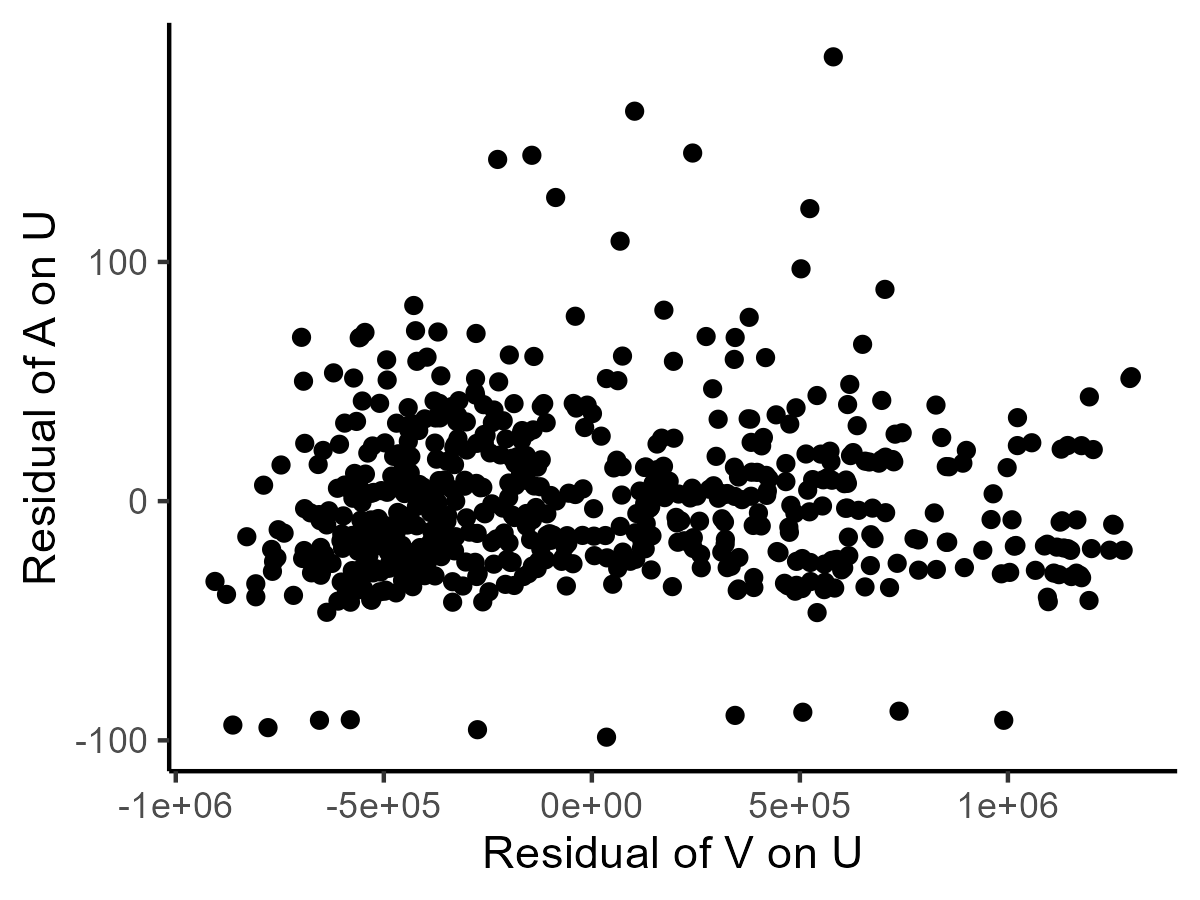
\includegraphics[width = 0.30\textwidth]
  {figuretable/residual_plot_month_aggregate.png}}
  % \subfloat[Year-level part-time and full-time]{\includegraphics[width = 0.30\textwidth]
  % {figuretable/residual_plot_year.png}}
  \subfloat[Full-time]{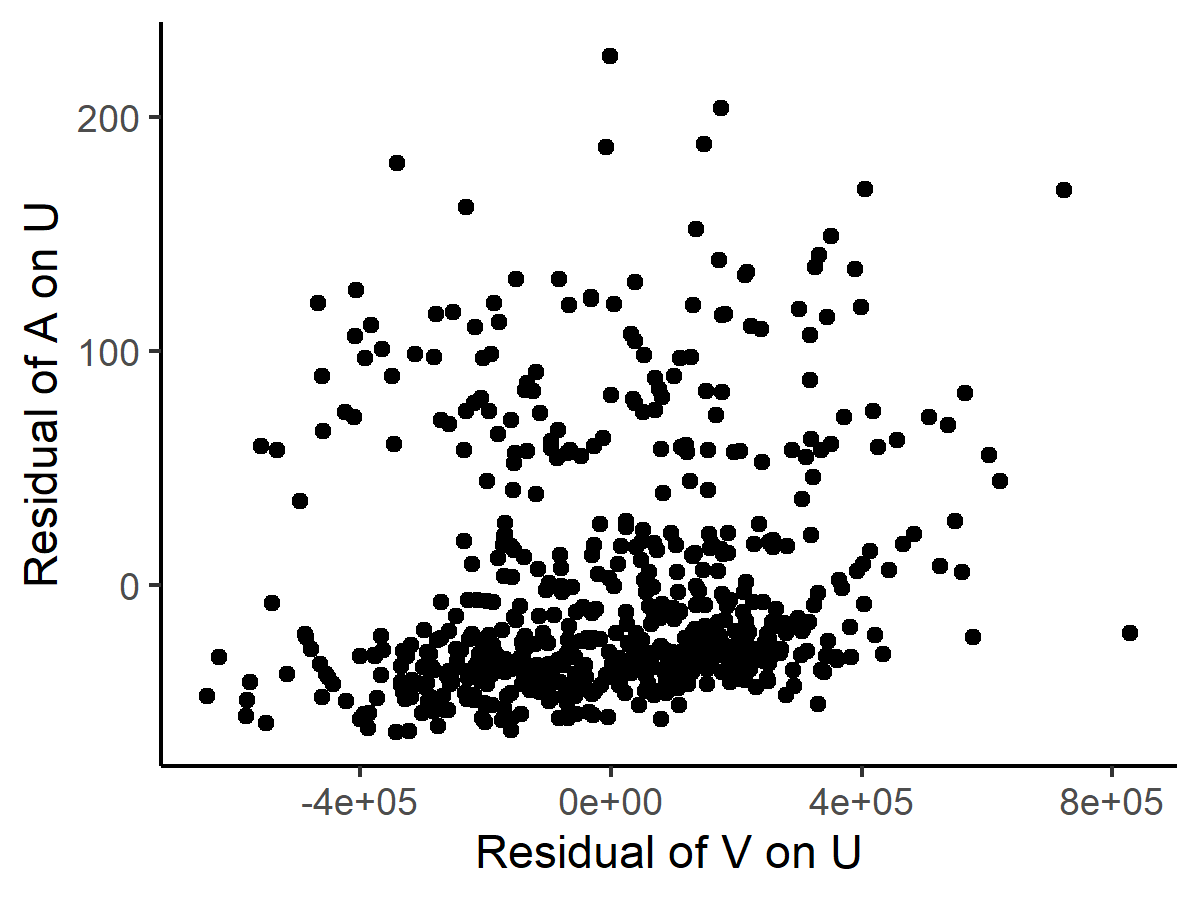
\includegraphics[width = 0.30\textwidth]
  {figuretable/residual_plot_month_full_time.png}}
  \subfloat[Part-time]{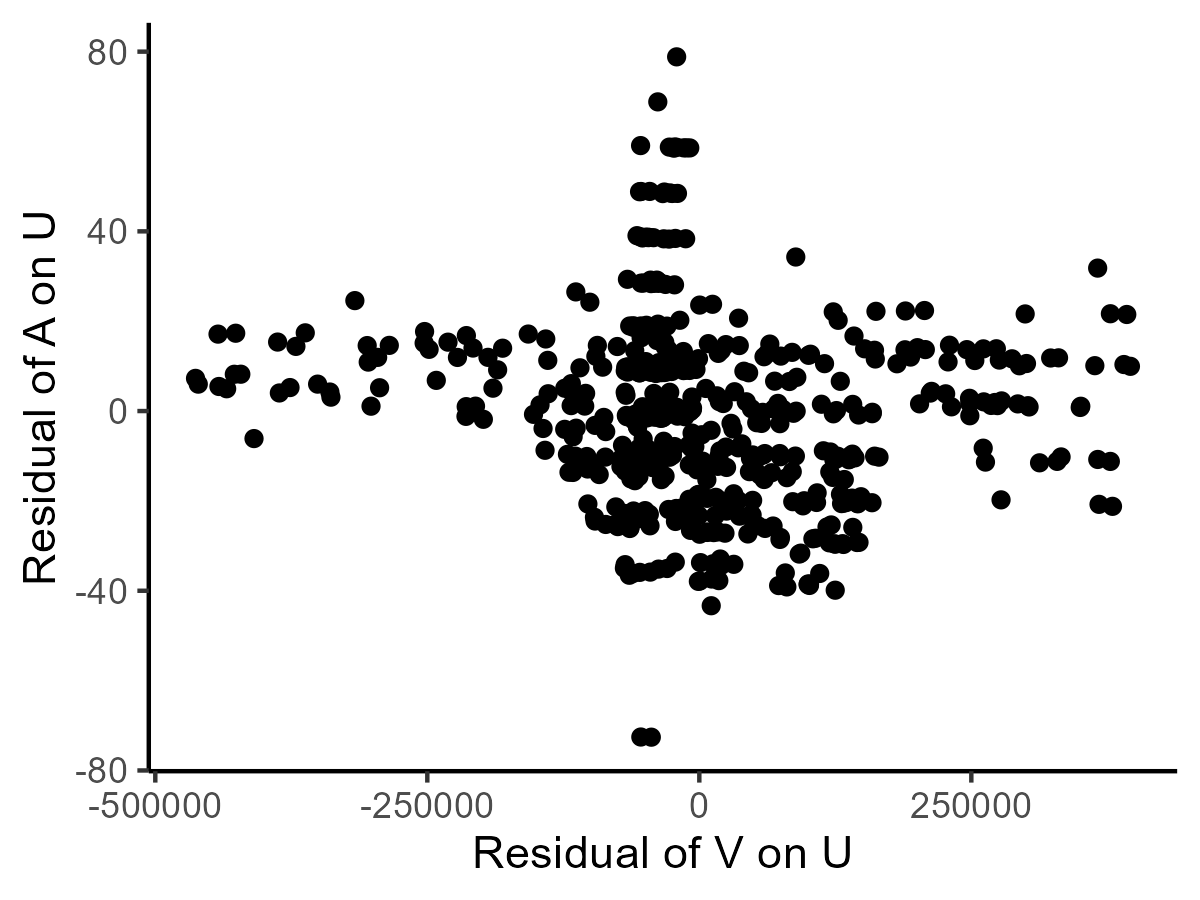
\includegraphics[width = 0.30\textwidth]
  {figuretable/residual_plot_month_part_time.png}}
  \caption{Residual plot}
  \label{fg:residual_plots} 
  \end{center}
  \footnotesize
  %Note: 
\end{figure} 




\subsection{Aggregate trends in 1972-2023}\label{sec:month_level}

Figures \ref{fg:month_part_and_full_time_results} (a)-(d) provide monthly data patterns of unemployed individuals, vacancies, labor market tightness (\(V/U\)), hires, the  ($U$,$V$) relationship, and job and worker finding rates (\(M/U\) and \(M/V\)) in aggregate labor markets. 
In summary, the numbers of unemployed individuals and vacancies increase with fluctuations, corresponding with market tightness, while the number of hires shows a noticeable decline around the late 1970s, peaks and troughs from the mid-1980s to the late 1990s, peaks around mid-2000s and 2010, and a sharp decline towards recent years.
Although the ($U$,$V$) relationship does not corresponds with Beveridge curve because these numbers are not divided by the corresponding number of labor force, the prominent rightward shifts are consistent with the previous studies \citep{elsby2015beveridge}.

Figures \ref{fg:month_part_and_full_time_results} (e) and (f) present the estimation results of the matching function along with matching efficiency and elasticities (\(\frac{d\ln M}{d\ln AU}\) and \(\frac{d\ln M}{d\ln V}\)). Notably, matching efficiency (normalized to 1972) shows a declining trend with notable fluctuations, which is consistent with the downward trends of job and worker finding rates. 
In particular, the significant decline after 2015 is remarkable.
This seems due to an increase in matching opportunities outside of the government-operated platform.

The implied match elasticity with respect to unemployment is 0.5-0.9, which is comparable to previous worldwide findings such as \cite{petrongolo2001looking} (range: 0.5-0.7) and Japanese studies such as \cite{higashi2018spatial} (0.38 for 2000-2014 monthly), \cite{kawata2019} (0.48 for 2012-2017 prefecture-month-level), \cite{kano2005estimating} (0.56 for 1972-1999 prefecture-year-level), \cite{sasaki2007measuring} (about 0.6 for 1998-2007 prefecture-quarter-level), and \cite{kambayashi2006vacancy} (about 0.8 for 1996-2001 prefecture-month-level).\footnote{For reference, \cite{petrongolo2001looking} summarize early aggregate studies in many countries based on a Cobb-Douglas matching function with the flow of hires on the left-hand side and the stock of unemployment and job vacancies on the right-hand side. In short, match elasticity with respect to unemployment is in the range of 0.5–0.7. \cite{bernstein2022matching} review the recent empirical literature that estimates the matching elasticity in the U.S. by four types of specification; Cobb-Douglas, Cobb-Douglas with endogeneity correction, a constant elasticity of substitution (CES), and nonparametric \citep{lange2020beyond}. The broad range of estimates is partly due to variations in data choices and periods. Higher estimates are typically derived from JOLTS data \citep{borowczyk2013accounting, csahin2014mismatch}, while lower estimates are often obtained from CPS flows data \citep{barnichon2015labor} or industry-level hires from CPS data \citep{csahin2014mismatch}.}
% However, I discuss the need for careful interpretation of the estimates due to scale normalization of matching efficiency in Section \ref{sec:month_level}.
On the other hand, the implied match elasticity with respect to vacancies is 0.1-0.4, which is comparable to \cite{lange2020beyond} (range: 0.15-0.3) and Japanese studies such as \cite{higashi2018spatial} (0.24 for 2000-2014 monthly), \cite{kawata2019} (0.52 for 2012-2017 prefecture-month-level), \cite{kano2005estimating} (0.3 for 1972-1999 prefecture-year-level), \cite{sasaki2007measuring} (about 0.2 for 1998-2007 prefecture-quarter-level), and \cite{kambayashi2006vacancy} (about 0.3 for 1996-2001 prefecture-month-level).

Figures \ref{fg:month_part_and_full_time_results} (g) and (h) illustrate some correlation patterns between matching efficiency and market structure variables such as labor market tightness, worker finding rate, and job finding rate. Consistent with \cite{lange2020beyond}, these highlight positive correlations between efficiency and market structure, such as tightness, which induce a positive bias in the estimates of the vacancy elasticity whenever unobserved matching efficiency is not controlled for, as is the case in traditional estimators.


\begin{figure}[!ht]
  \begin{center}
  \subfloat[Unemployed ($U$), Vacancy ($V$), and Tightness ($\frac{V}{U}$)]{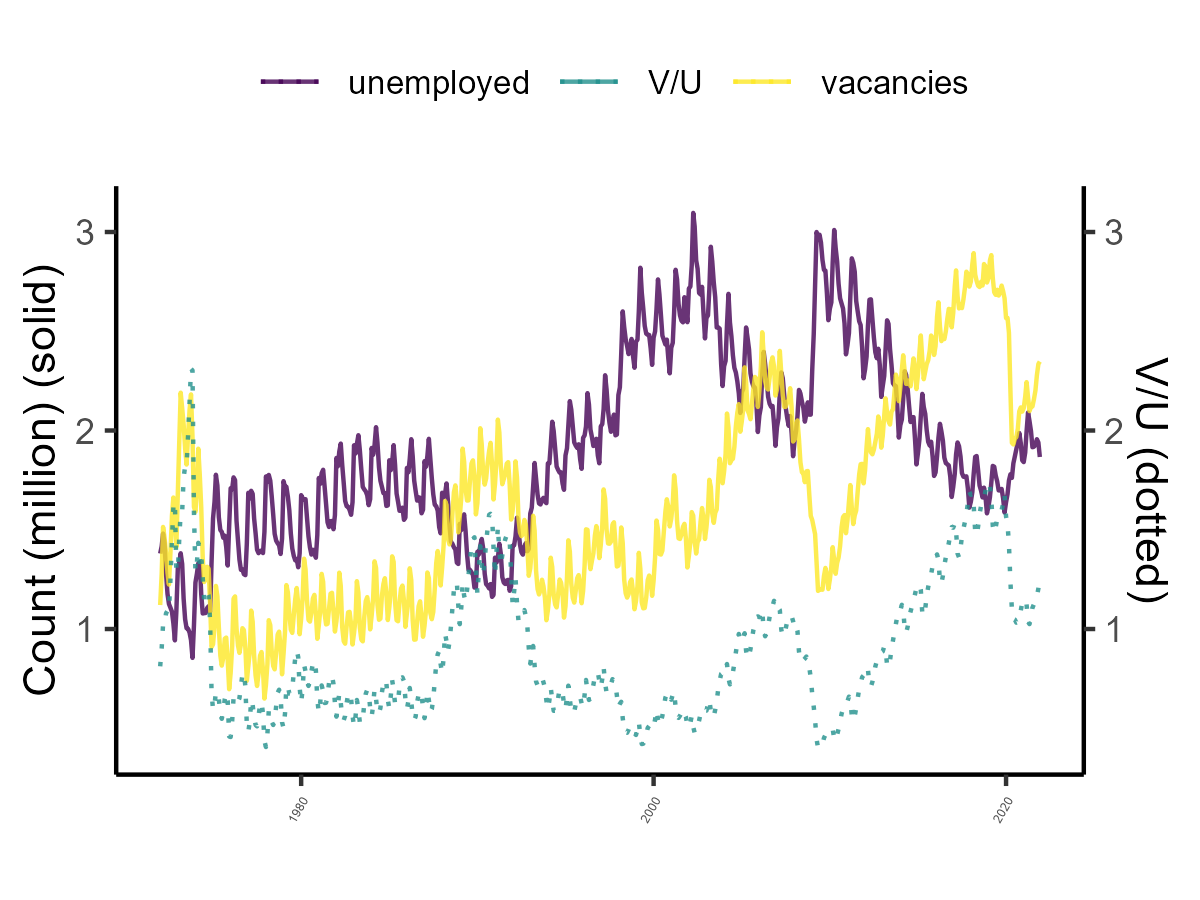
\includegraphics[width = 0.37\textwidth]
  {figuretable/unemployed_vacancy_month_aggregate.png}}
  \subfloat[Hire ($H$)]{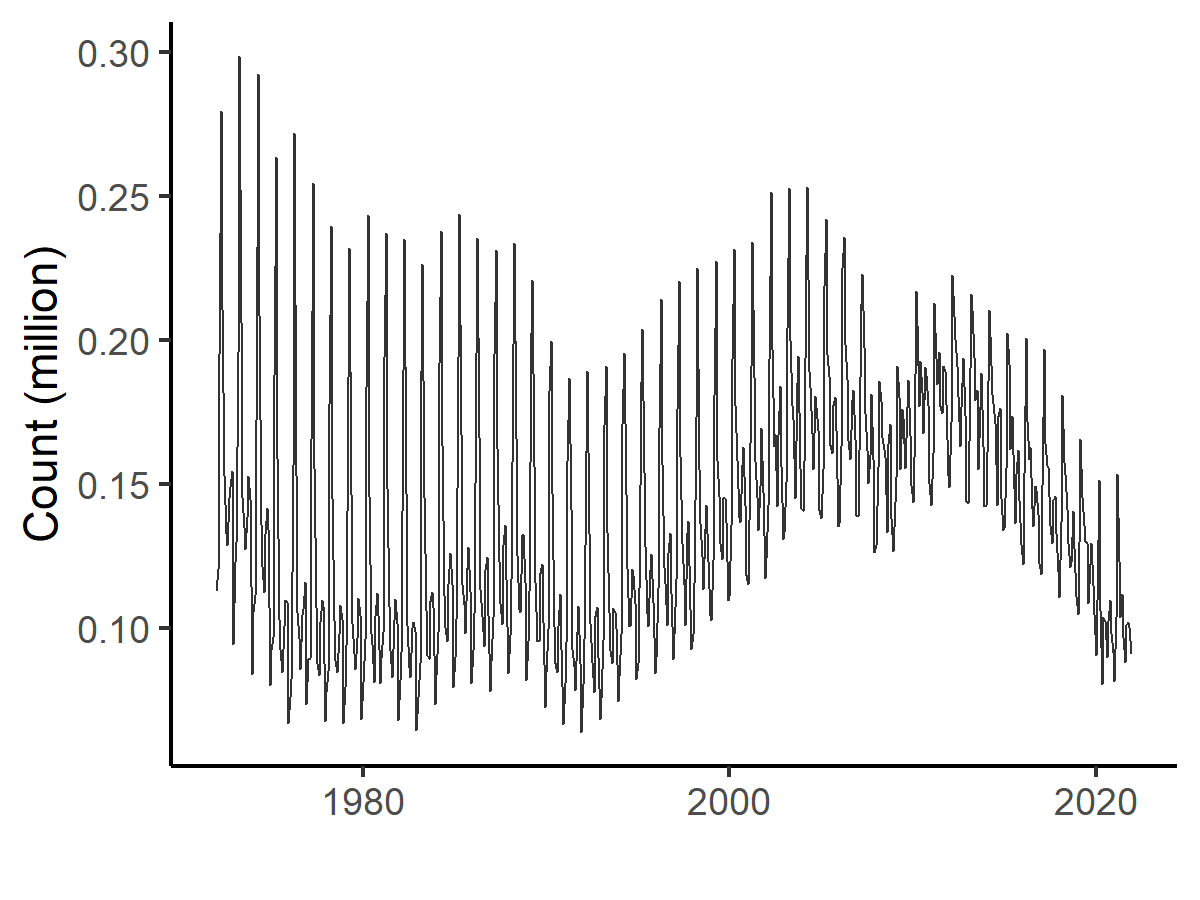
\includegraphics[width = 0.37\textwidth]
  {figuretable/hire_month_aggregate.png}}\\
  \subfloat[ ($U$,$V$) relationship]{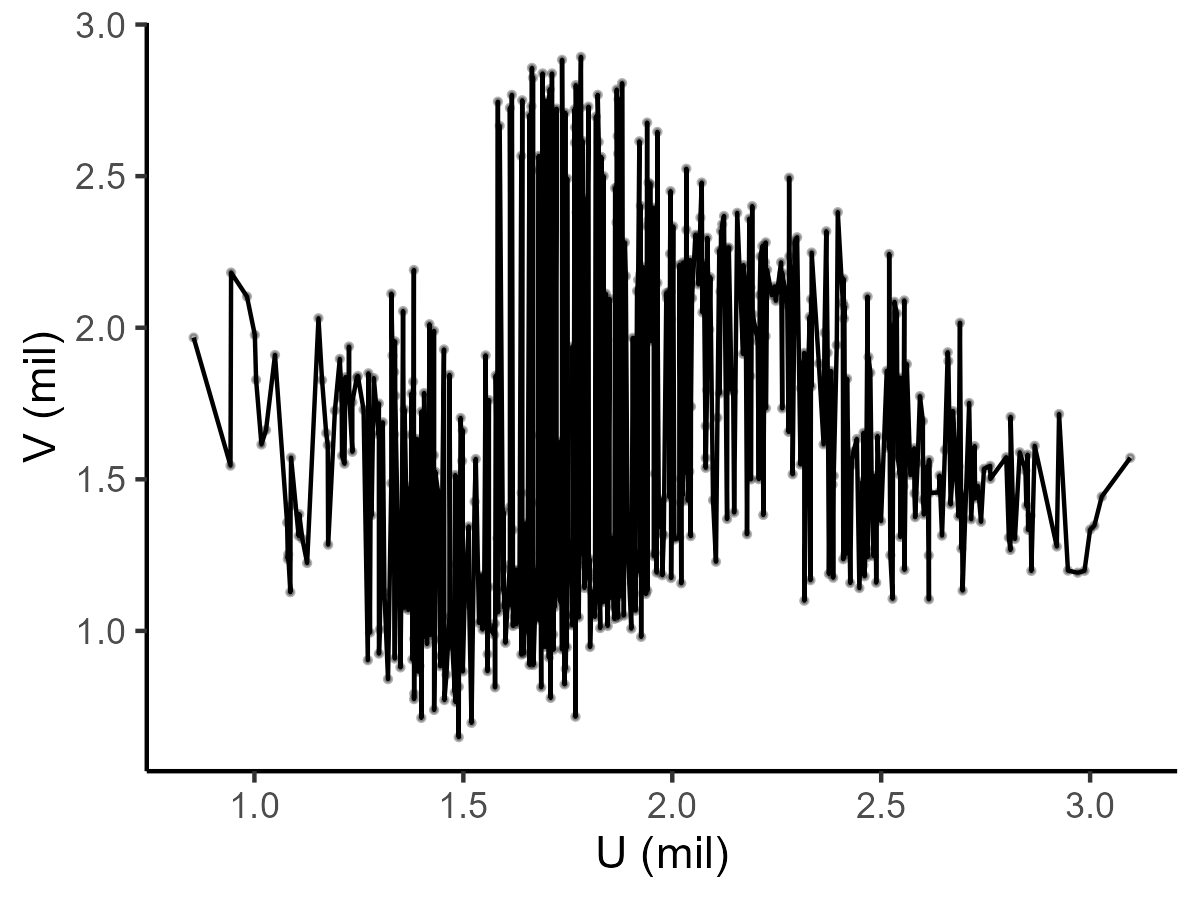
\includegraphics[width = 0.37\textwidth]
  {figuretable/unemployed_vacancies_berveridge_month_aggregate.png}}
  \subfloat[Job Worker finding rate ($\frac{M}{U}$,$\frac{M}{V}$)]{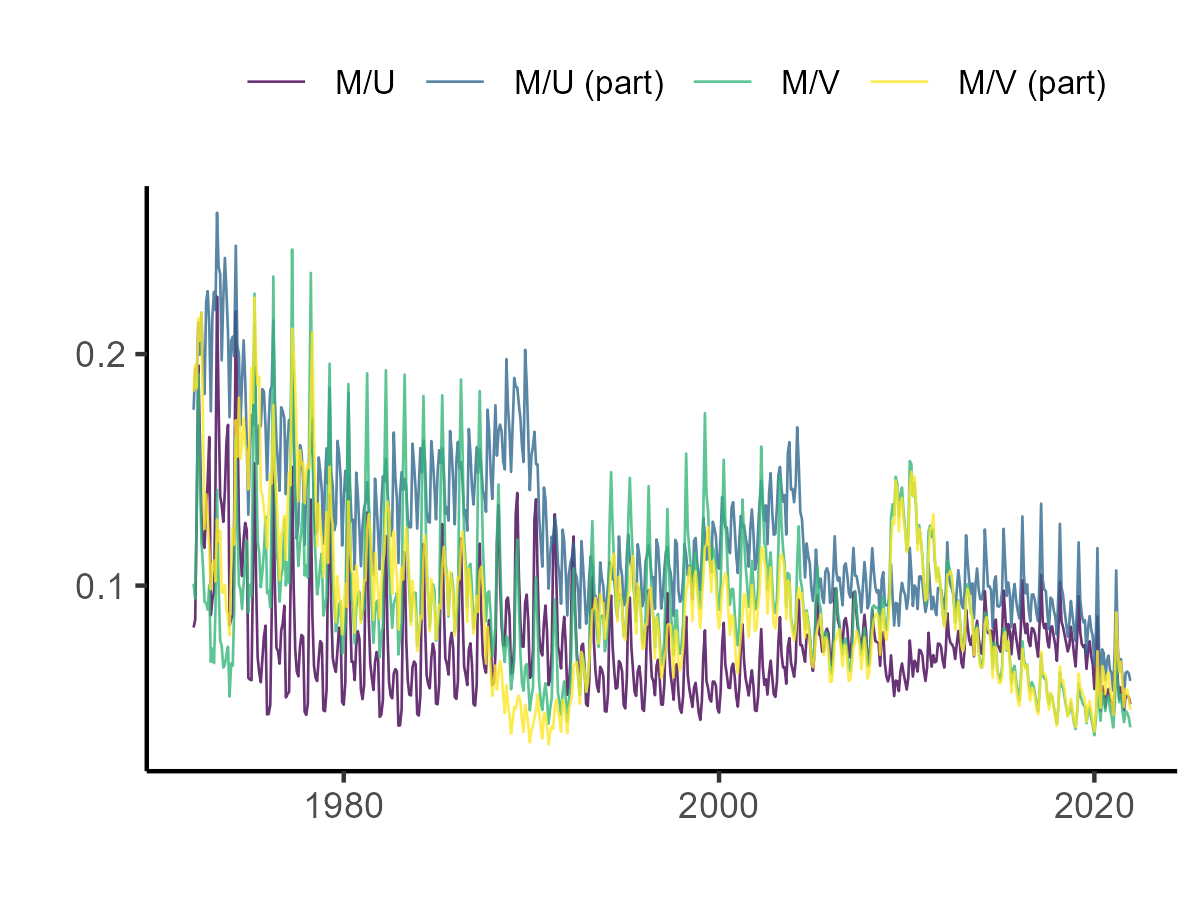
\includegraphics[width = 0.37\textwidth]
  {figuretable/job_finding_rate_worker_finding_rate_month_aggregate.png}}
  \\
  \subfloat[Matching Efficiency ($A$)]{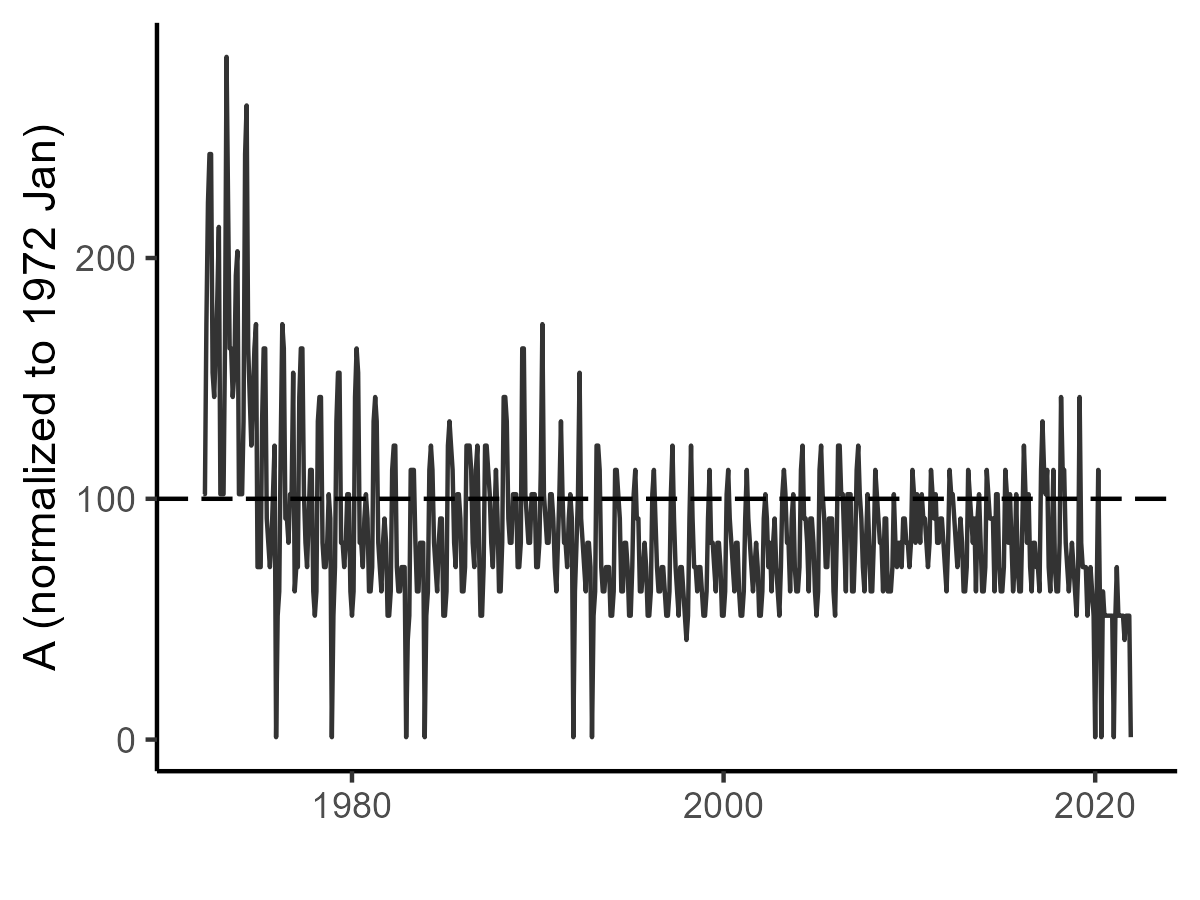
\includegraphics[width = 0.37\textwidth]
  {figuretable/matching_efficiency_month_aggregate.png}}
  \subfloat[Matching Elasticity ($\frac{d\ln M}{d \ln AU}$, $\frac{d\ln M}{d\ln V}$)]{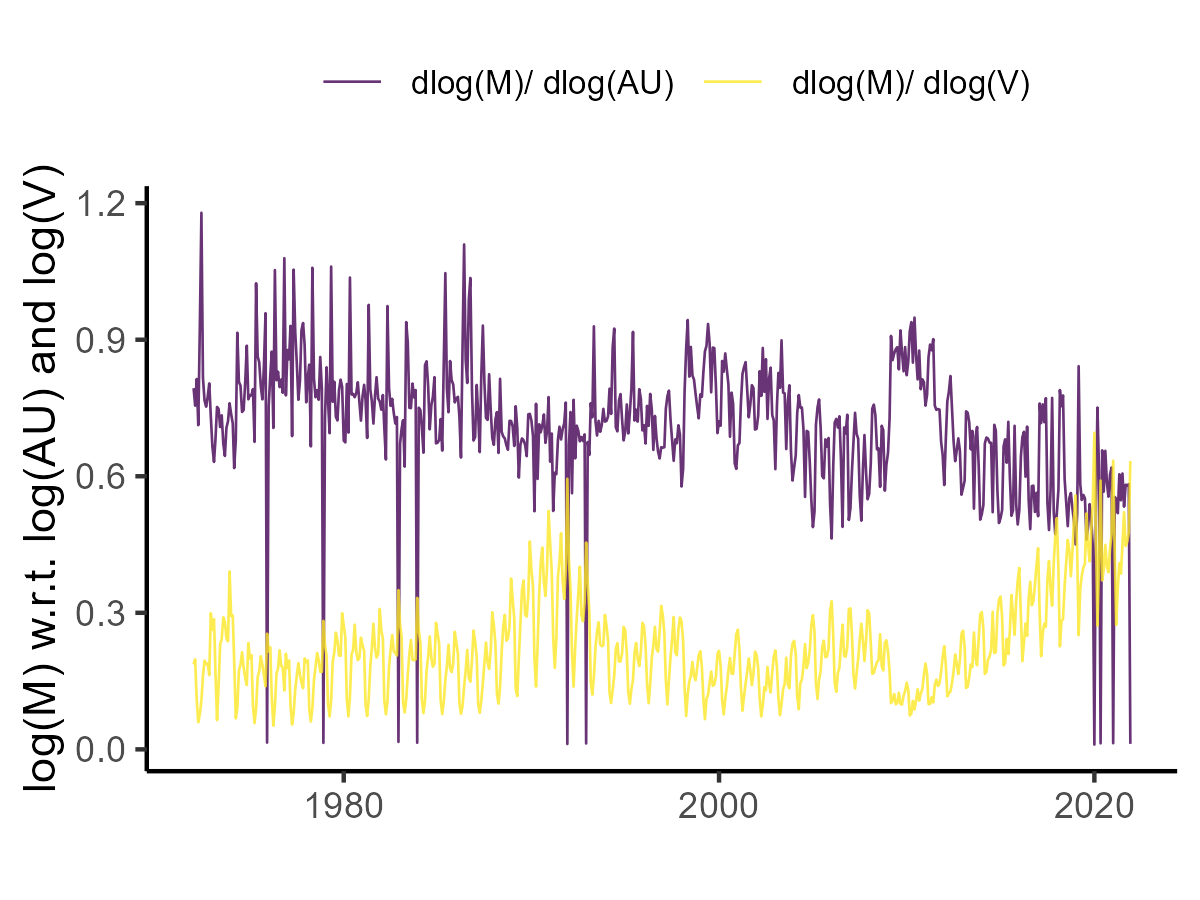
\includegraphics[width = 0.37\textwidth]
  {figuretable/elasticity_month_aggregate.png}}\\
  \subfloat[Efficiency ($A$) and Tightness ($\ln\frac{V}{U}$)]{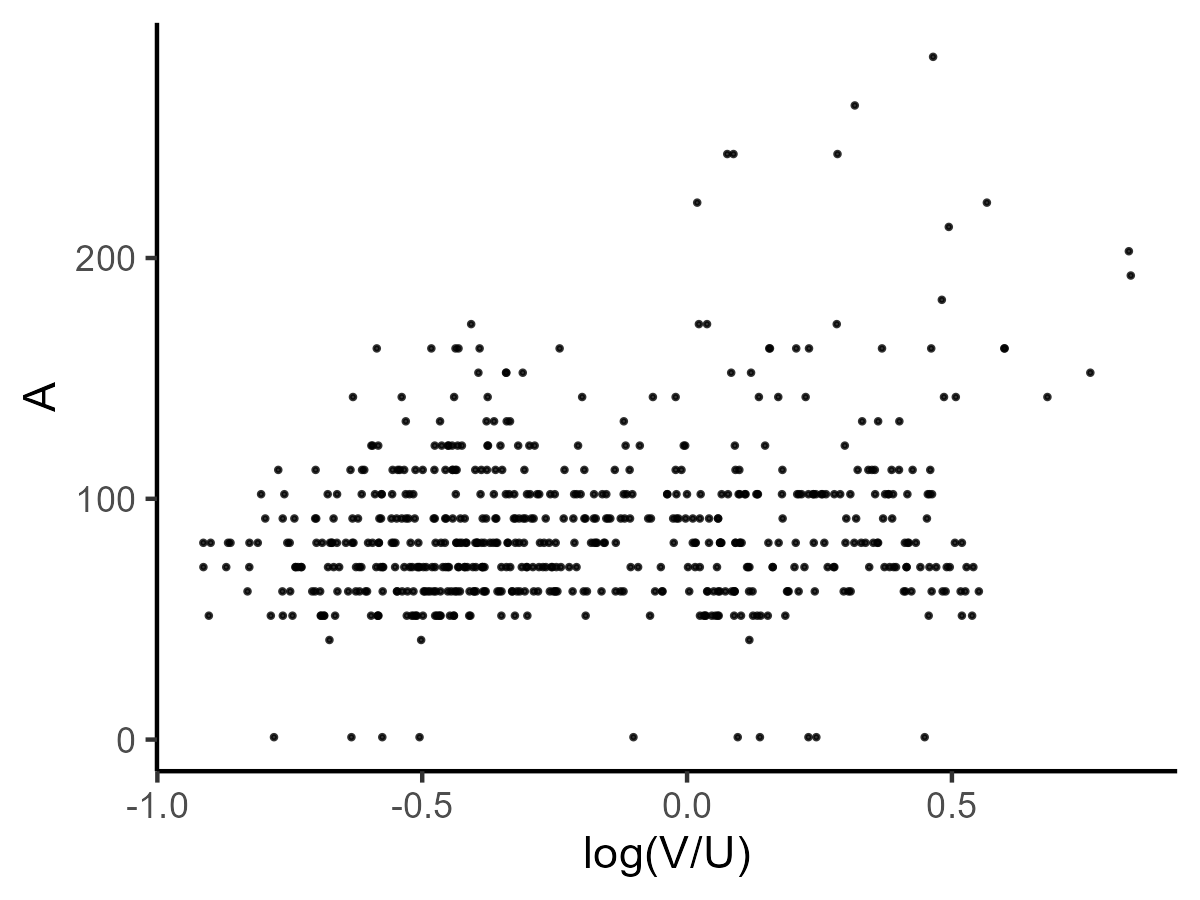
\includegraphics[width = 0.37\textwidth]
  {figuretable/efficiency_tightness_plot_month_aggregate.png}}
  \subfloat[Efficiency ($A$) and ($\ln\frac{M}{U}$, $\ln\frac{M}{V}$)]{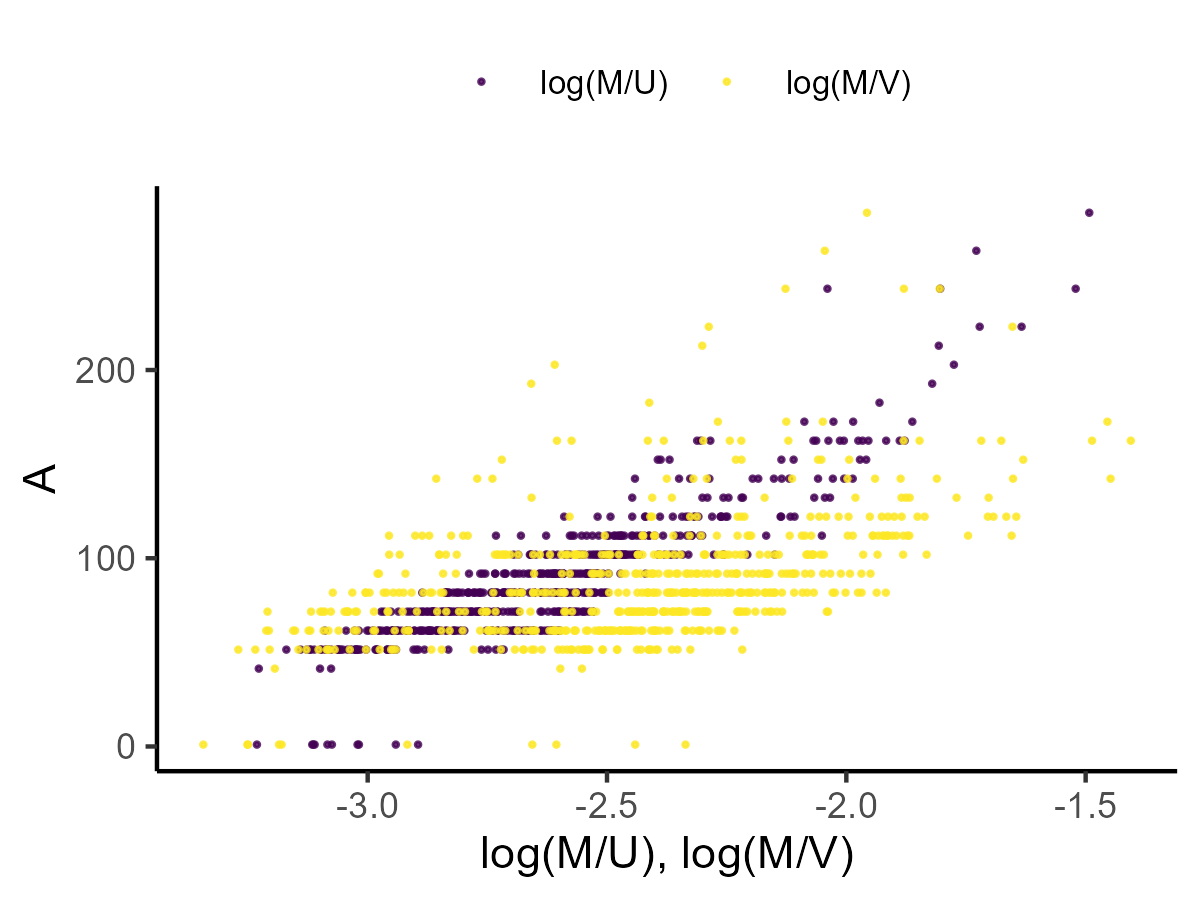
\includegraphics[width = 0.37\textwidth]
  {figuretable/job_finding_rate_efficiency_plot_month_aggregate.png}}
  \caption{Month-level aggregate results 1972-2024}
  \label{fg:month_part_and_full_time_results} 
  \end{center}
  \footnotesize
  %Note: 
\end{figure} 




\subsection{Decomposition of part-time and full time trends in 1972-2023}
Next, we decompose the aggregate trends into full-time and part-time labor markets' trends.
Figure \ref{fg:month_full_time_part_time_results} provide full-time and part-time labor markets' trends corresponding Figures \ref{fg:month_part_and_full_time_results} (a)-(f).
Panel (a) shows that full-time unemployment and vacancies show higher counts and more significant fluctuations compared to part-time data and that part-time unemployment and vacancies exhibit a more gradual and steady trend over the years.
Both full-time and part-time labor markets experience periods of high tightness during the same general periods, notably in the early 1990s.
Part-time labor market tightness shows more pronounced peaks compared to the full-time labor market.
Panel (b) shows that the sharp decline in full-time hires post-2008 suggests greater sensitivity to economic downturns and structural changes in the labor market.
The steady rise in part-time hires indicates increasing reliance on part-time employment, possibly due to greater flexibility and adaptability in the labor market.
Panel (c) illustrates that full-time employment data covers a wider range of both unemployed and vacancies, indicating higher variability in the full-time labor market in contrast to a more stable part-time labor market.
Panel (d) shows that full-time finding rates show higher initial values and more significant declines compared to part-time finding rates.
Part-time finding rates demonstrate a more gradual decline and stable fluctuations over time.
Full-time finding rates exhibit larger fluctuations and more pronounced declines, indicating greater sensitivity to economic changes.
Part-time finding rates, while also showing initial declines, stabilize earlier and display less volatility, suggesting a more resilient part-time labor market.

Given estimation results in each dataset, Figure \ref{fg:month_full_time_part_time_correlation_results} (e) depicts the trend of implied matching efficiency.
The downward trends are common.
Full-time matching efficiency fluctuates from 80\% to 300\%, whereas part-time matching efficiency remains stable at 60\% compared to January 1972.
This concludes that the sharp decline of matching efficiency after COVID-19 shown in the aggregate trend is driven by the decline of full-time matching efficiency.

Figure \ref{fg:month_full_time_part_time_correlation_results} (f) depicts the trends of matching elasticities.
For matching elasticity with respect to unemployed, the full-time trend exhibits significant fluctuations, especially before the 1980s, ranging from 0.2 to around 1.0, indicating varying sensitivity of matching efficiency to changes in unemployment over time. 
In contrast, the part-time trend peaks, ranging from 0.9 to 1.0 after 2020, which may indicate the post-COVID effect on the elasticity.
For matching elasticity with respect to vacancy, the full-time trend shows a relatively stable trend, starting around 0.2, with slight increases in recent years, whereas the part-time trend maintains lower and more stable values around 0.1 to 0.3, suggesting that vacancies have a less pronounced effect on matching efficiency in the part-time labor market.

Figure \ref{fg:month_full_time_part_time_correlation_results} illustrates some correlation patterns between matching efficiency and market structure variables corresponding with Figures \ref{fg:month_part_and_full_time_results} (g)-(h).
I find the stronger and more consistent relationships in the full-time labor market.
This confirms that positive correlations between efficiency and market structure driven mainly by full-time markets.



\begin{figure}[!ht]
  \begin{center}
  \subfloat[Unemployed ($U$), Vacancy ($V$), and Tightness ($\frac{V}{U}$)]{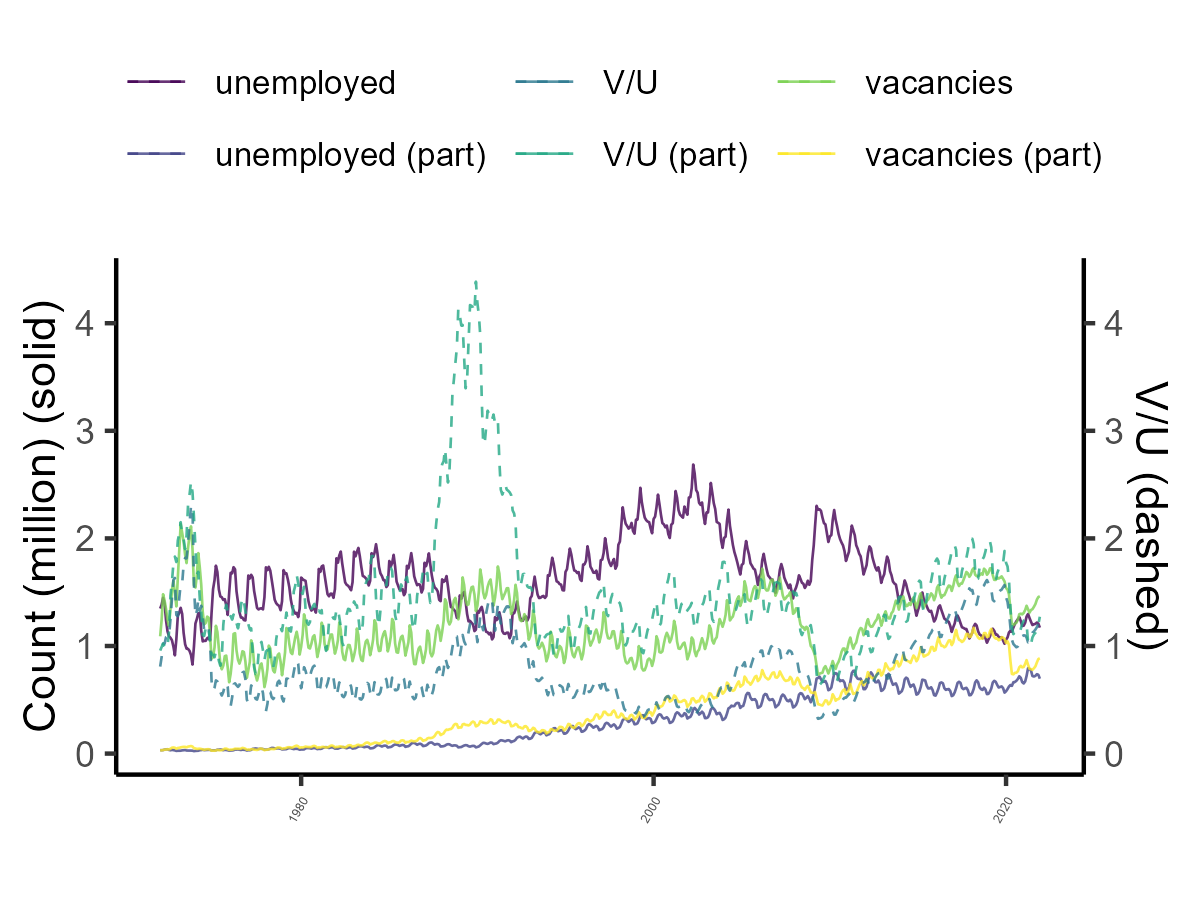
\includegraphics[width = 0.37\textwidth]
  {figuretable/unemployed_vacancy_month_full_time_part_time.png}}
  \subfloat[Hire ($H$)]{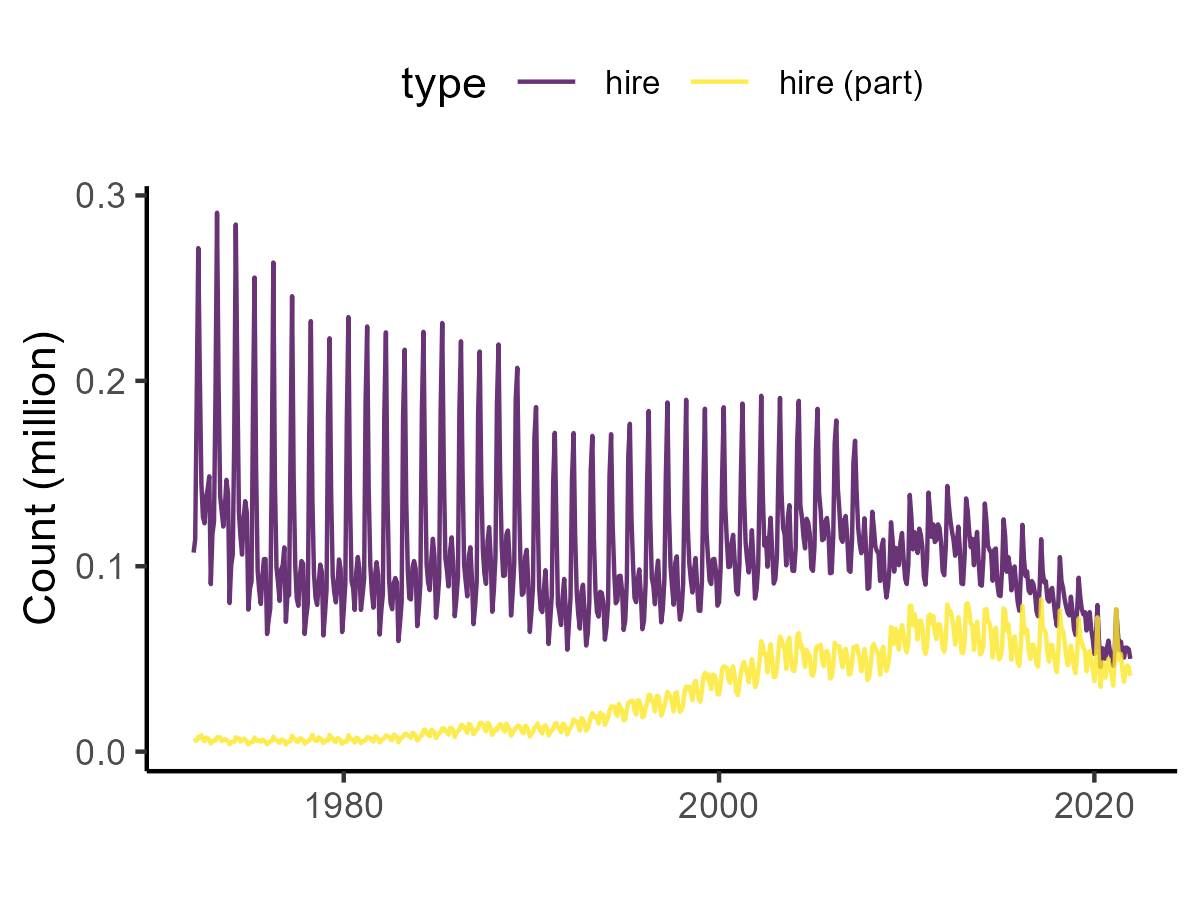
\includegraphics[width = 0.37\textwidth]
  {figuretable/hire_month_full_time_part_time.png}}\\
  \subfloat[ ($U$,$V$) relationship]{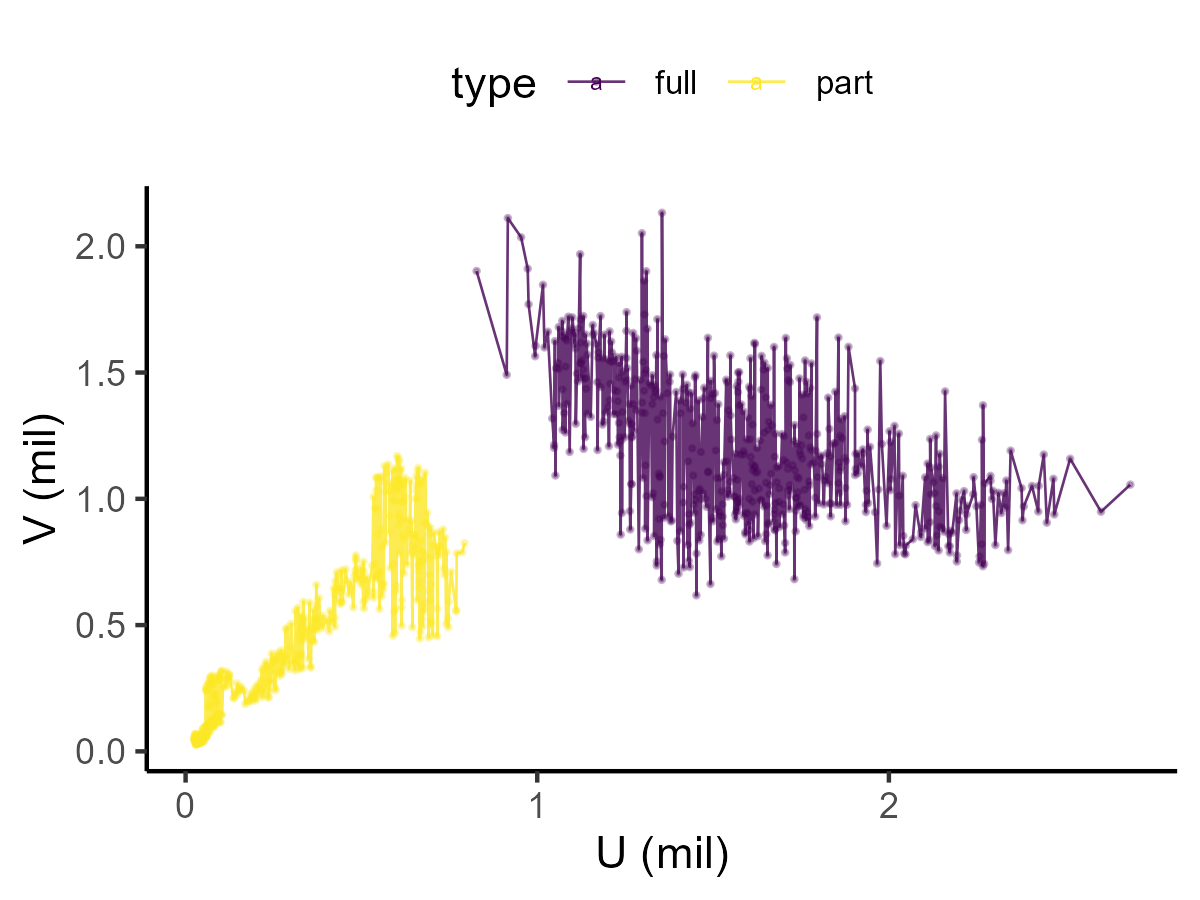
\includegraphics[width = 0.37\textwidth]
  {figuretable/unemployed_vacancies_berveridge_month_full_time_part_time.png}}
  \subfloat[Job Worker finding rate ($\frac{M}{U}$,$\frac{M}{V}$)]{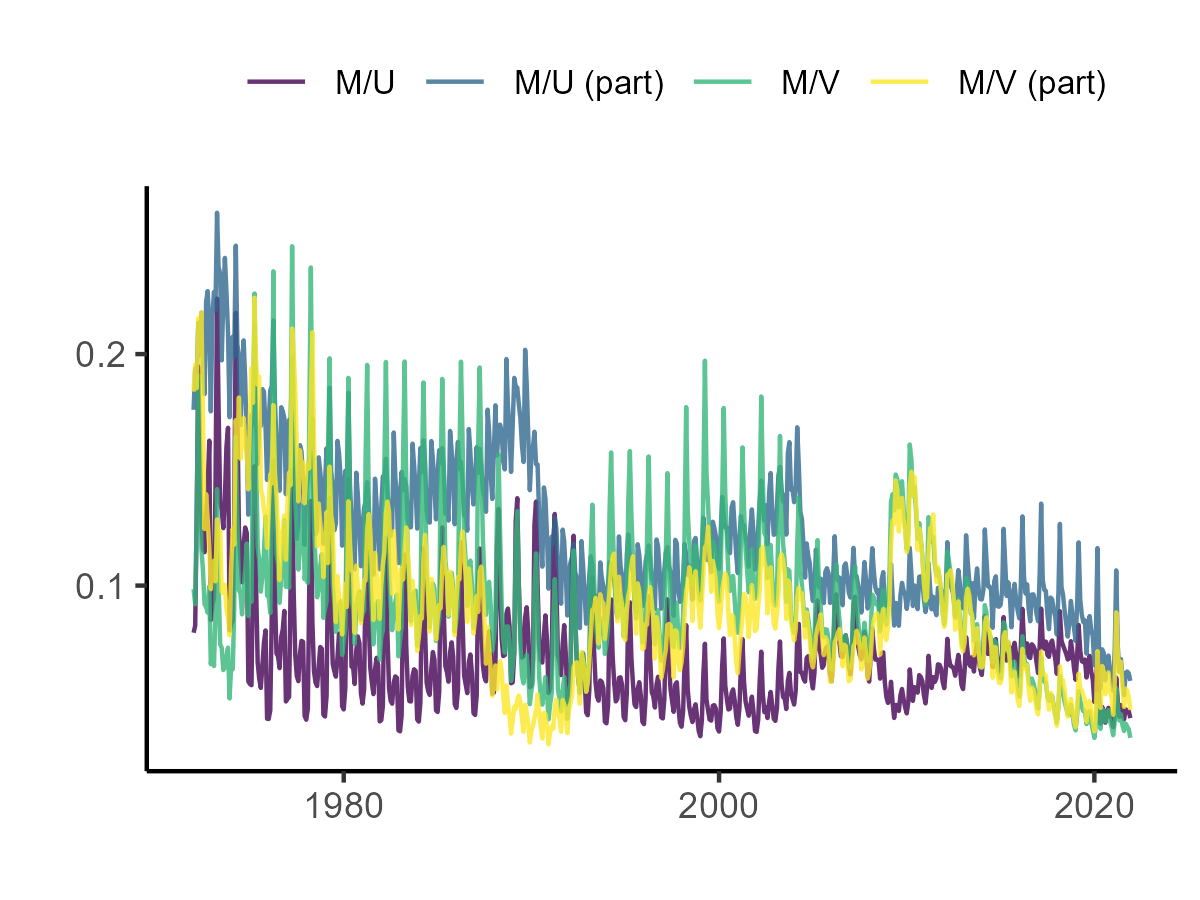
\includegraphics[width = 0.37\textwidth]
  {figuretable/job_finding_rate_worker_finding_rate_month_full_time_part_time.png}}
  \\
  \subfloat[Matching Efficiency ($A$)]{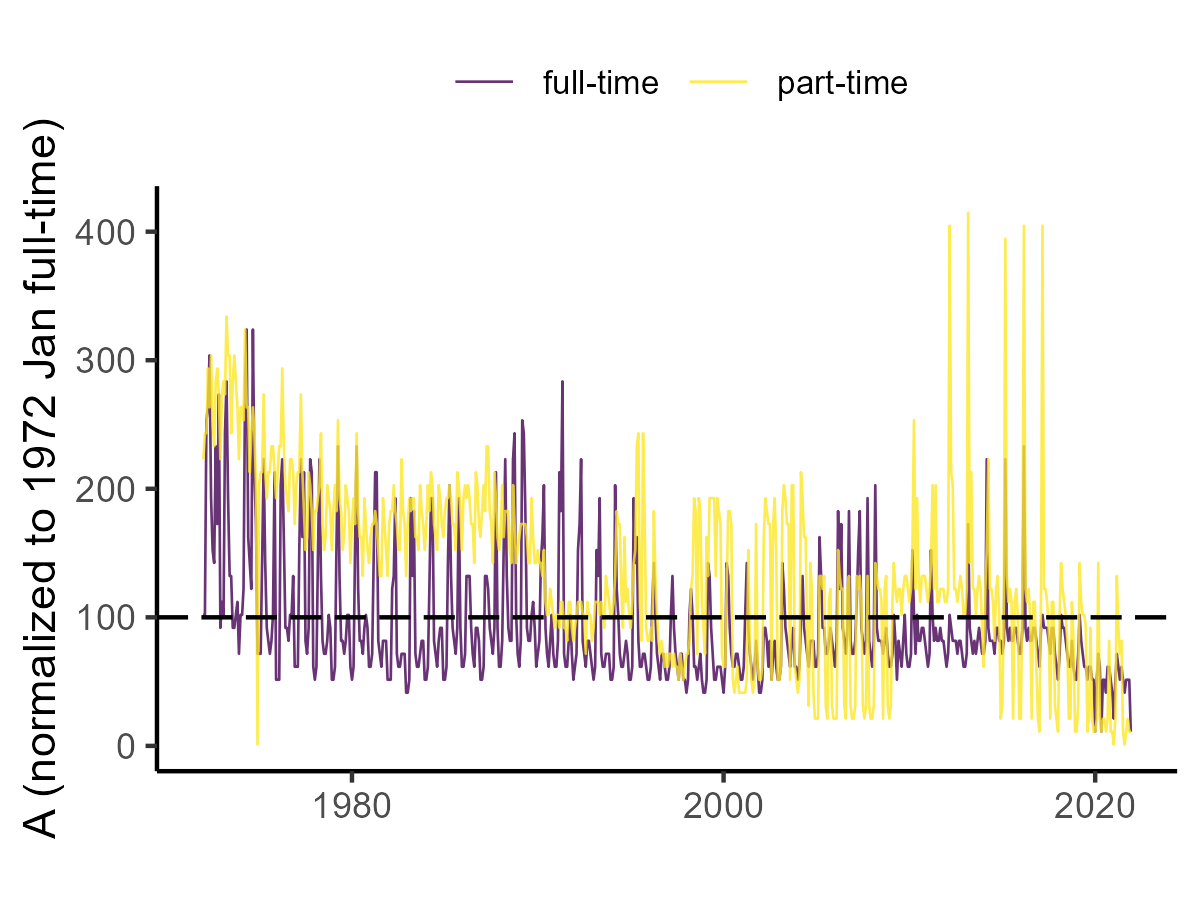
\includegraphics[width = 0.37\textwidth]
  {figuretable/matching_efficiency_month_full_time_part_time.png}}
  \subfloat[Matching Elasticity ($\frac{d\ln M}{d \ln AU}$, $\frac{d\ln M}{d\ln V}$)]{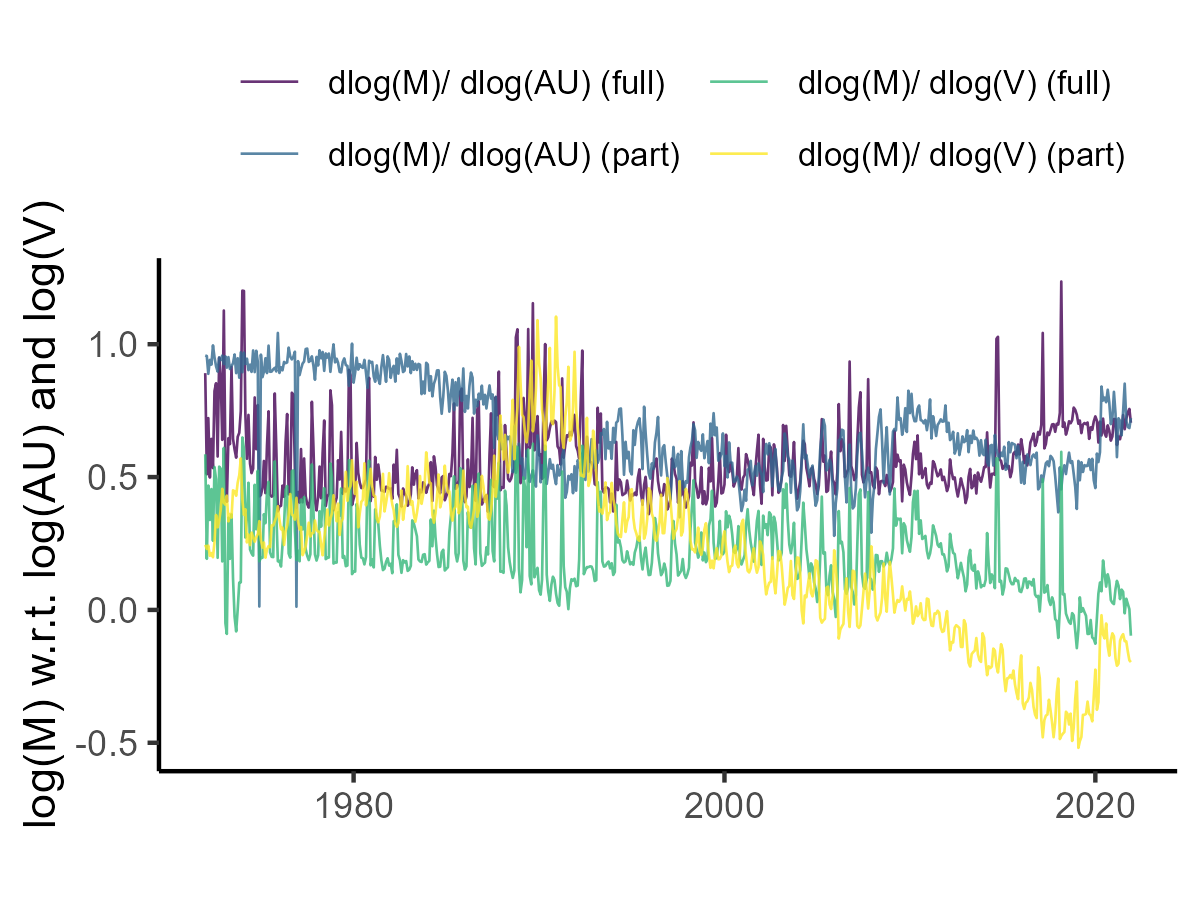
\includegraphics[width = 0.37\textwidth]
  {figuretable/elasticity_month_full_time_part_time.png}}
  \caption{Month-level full-time and part-time results 1972-2024}
  \label{fg:month_full_time_part_time_results} 
  \end{center}
  \footnotesize
  %Note: 
\end{figure} 


\begin{figure}[!ht]
  \begin{center}
  \subfloat[Efficiency ($A$) and Tightness ($\ln\frac{V}{U}$), Full-time (left) and Part-time (right)]{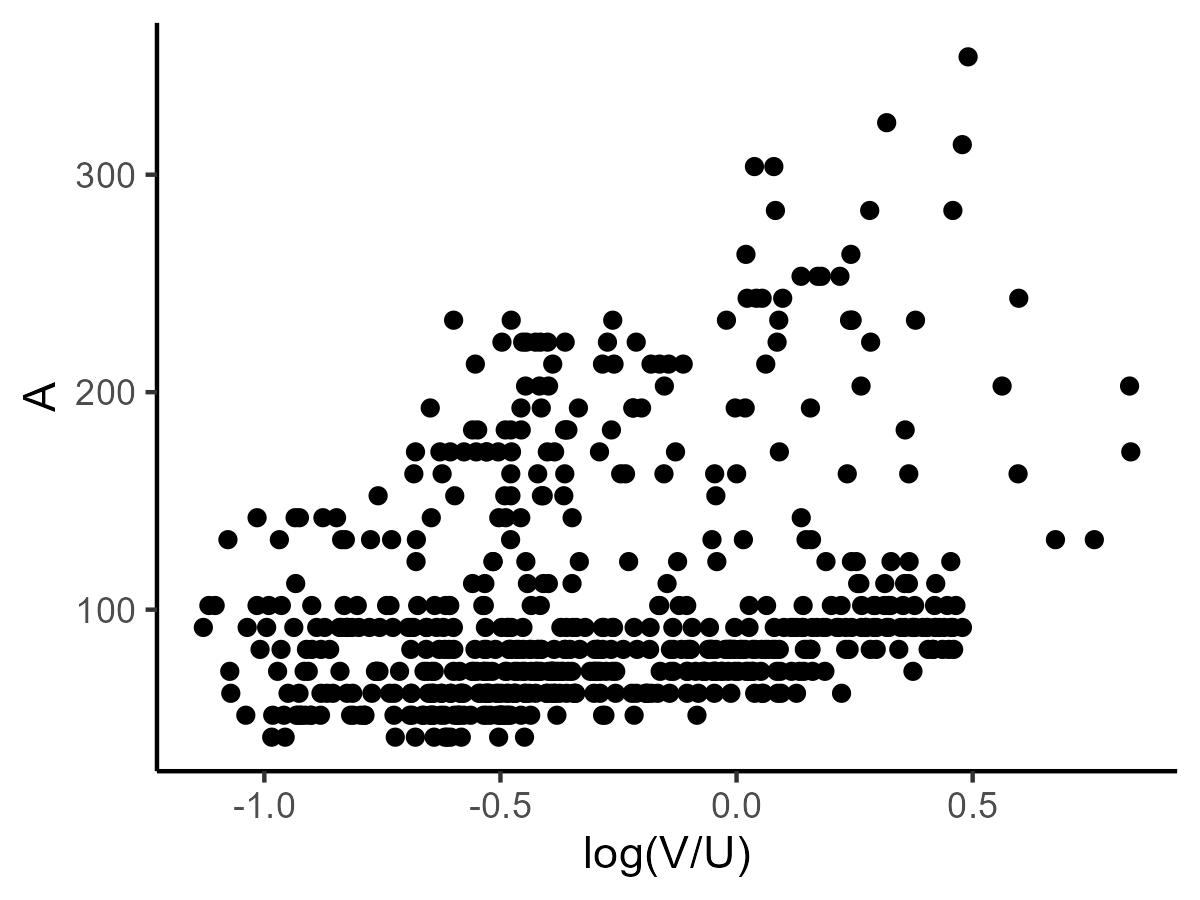
\includegraphics[width = 0.37\textwidth]
  {figuretable/efficiency_tightness_plot_month_full_time.png}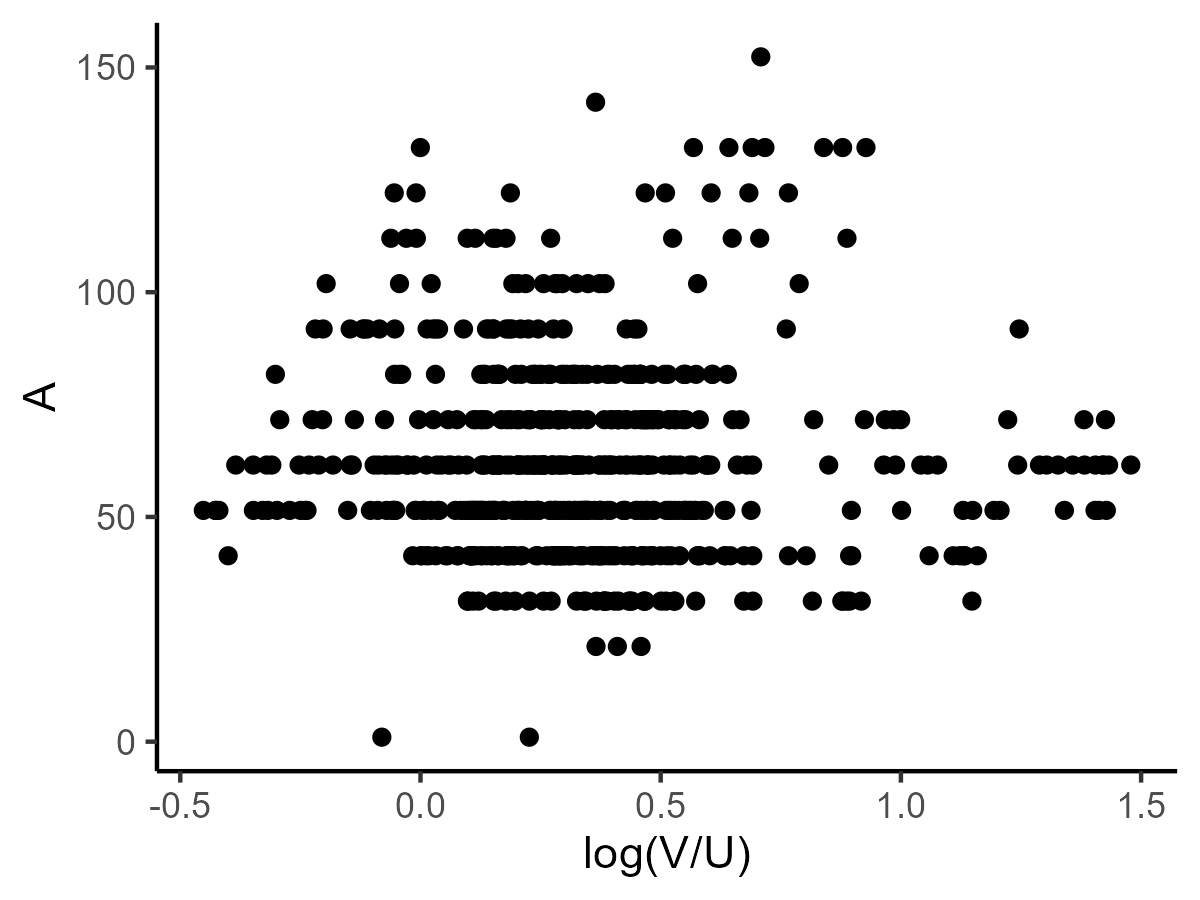
\includegraphics[width = 0.37\textwidth]
  {figuretable/efficiency_tightness_plot_month_part_time.png}}\\
  \subfloat[Efficiency ($A$) and ($\ln\frac{M}{U}$, $\ln\frac{M}{V}$), Full-time (left) and Part-time (right)]{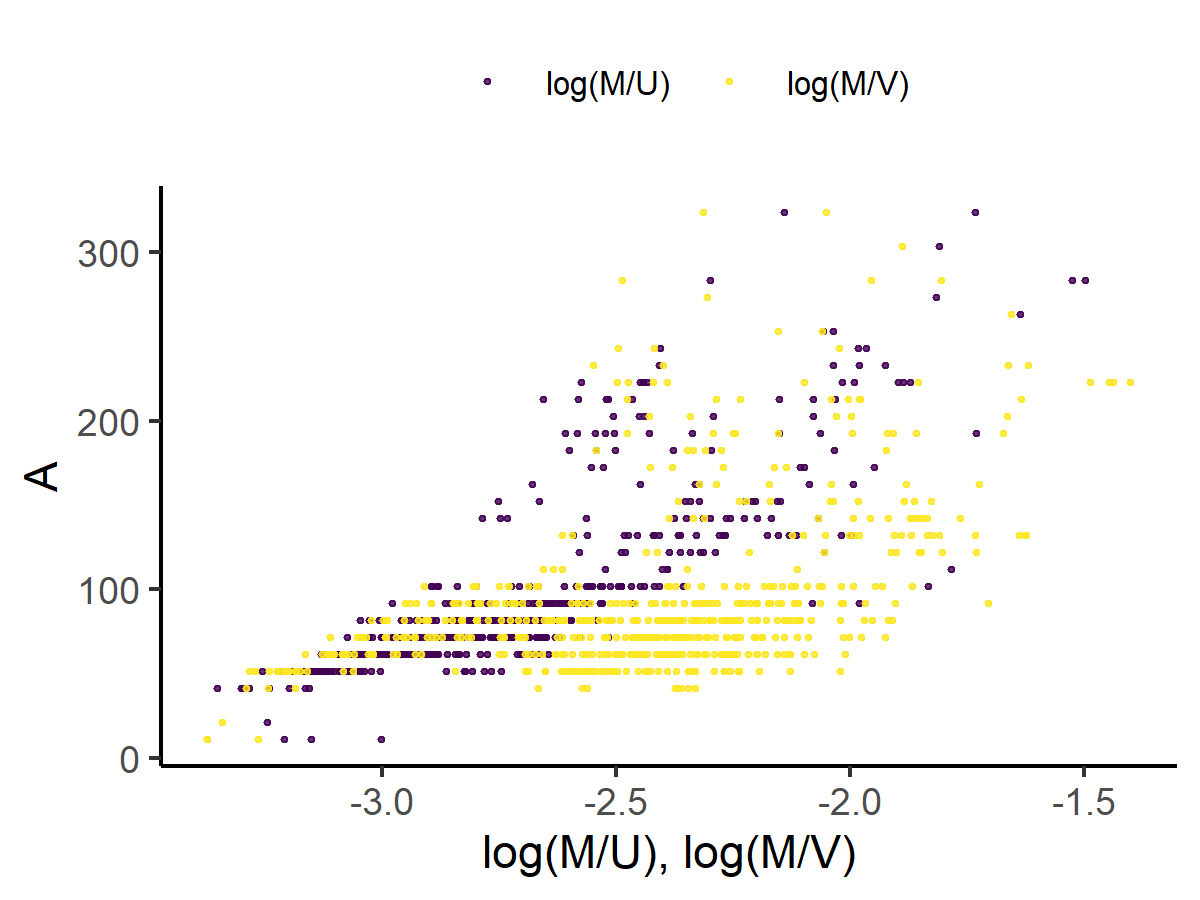
\includegraphics[width = 0.37\textwidth]
  {figuretable/job_finding_rate_efficiency_plot_month_full_time.png}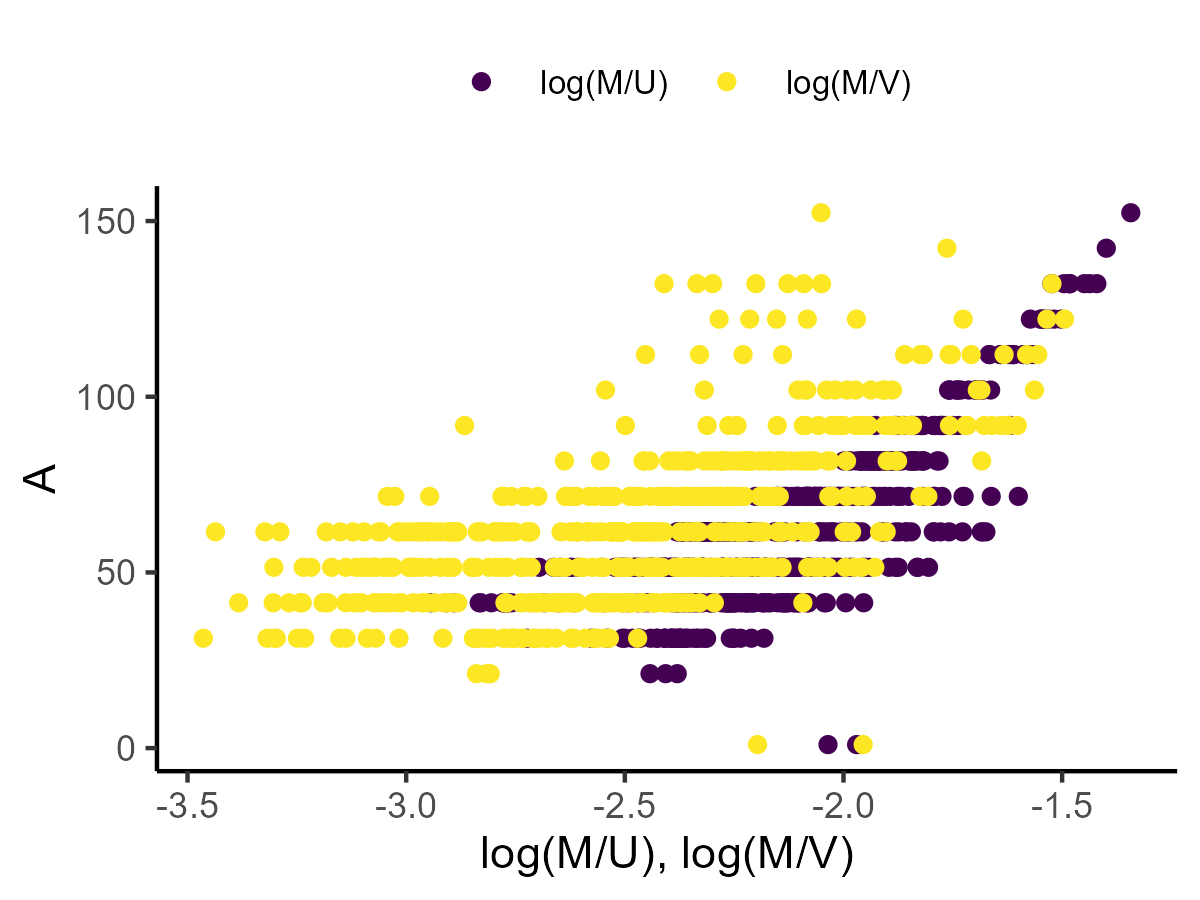
\includegraphics[width = 0.37\textwidth]
  {figuretable/job_finding_rate_efficiency_plot_month_part_time.png}}
  \caption{Month-level full-time and part-time results 1972-2024 (Continued)}
  \label{fg:month_full_time_part_time_correlation_results} 
  \end{center}
  \footnotesize
  %Note: 
\end{figure} 





\subsection{Prefecture-level aggregate results in 2012-2024}

Figure \ref{fg:month_part_and_full_time_matching_efficiency_prefecture_results}



\begin{figure}[!ht]
  \begin{center}
  \subfloat[Hokkaido]{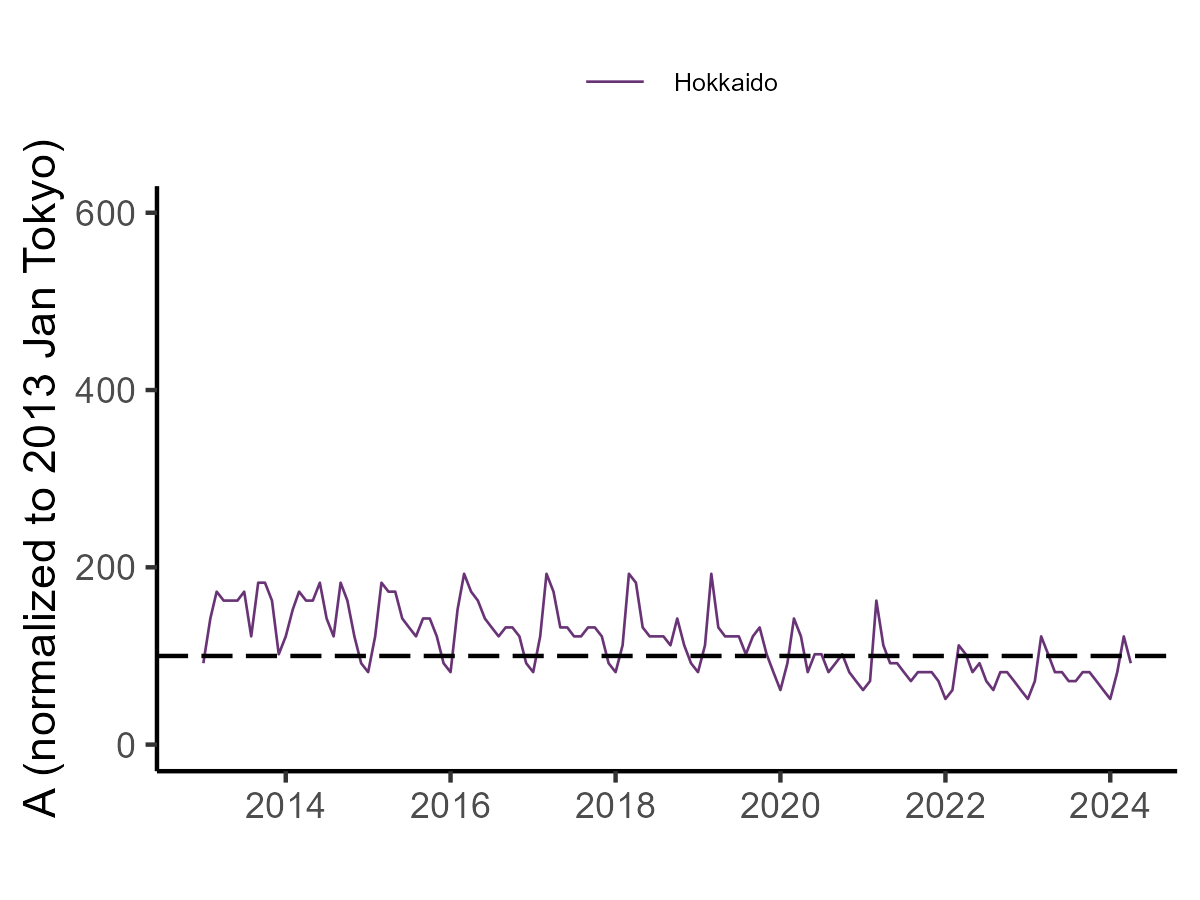
\includegraphics[width = 0.37\textwidth]
  {figuretable/matching_efficiency_month_aggregate_hokkaido.png}}
  \subfloat[Tohoku]{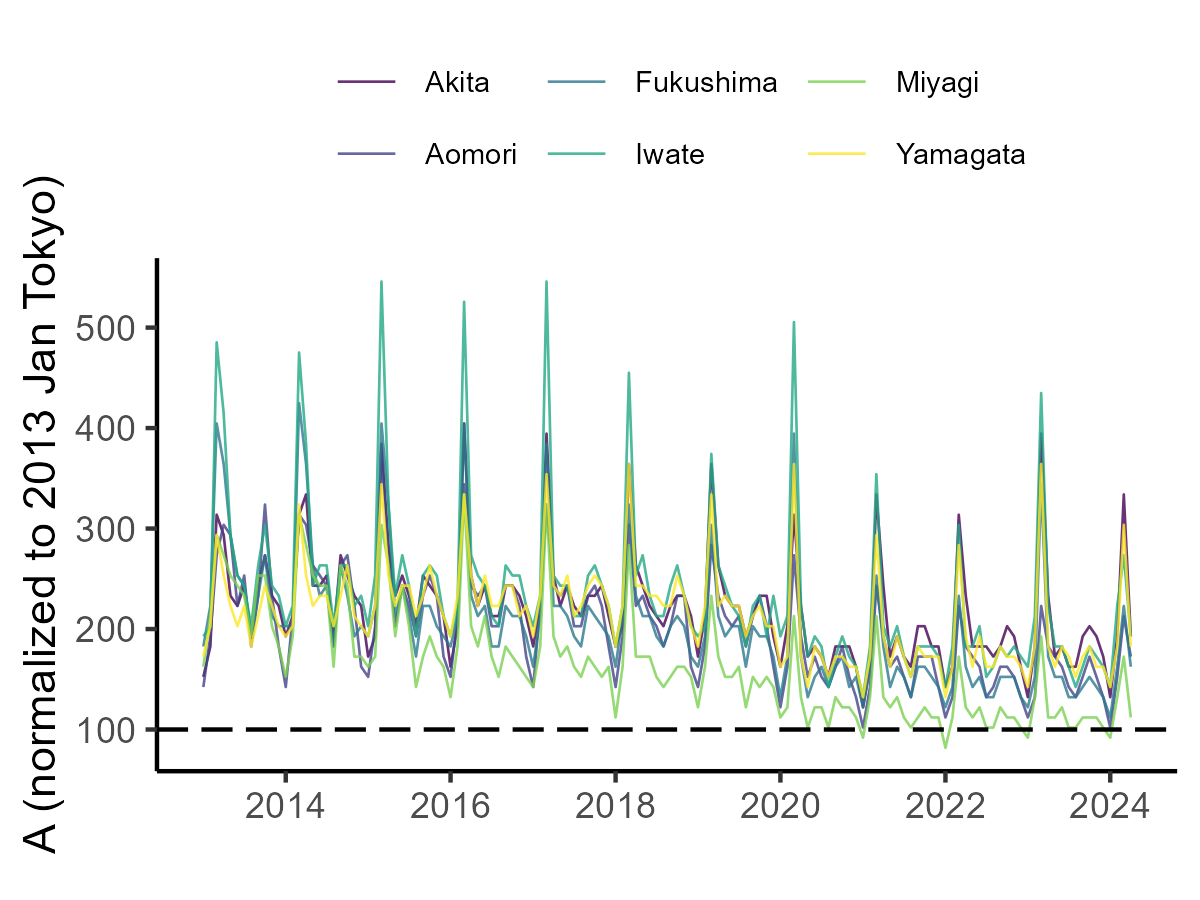
\includegraphics[width = 0.37\textwidth]
  {figuretable/matching_efficiency_month_aggregate_tohoku.png}}\\
  \subfloat[Kanto]{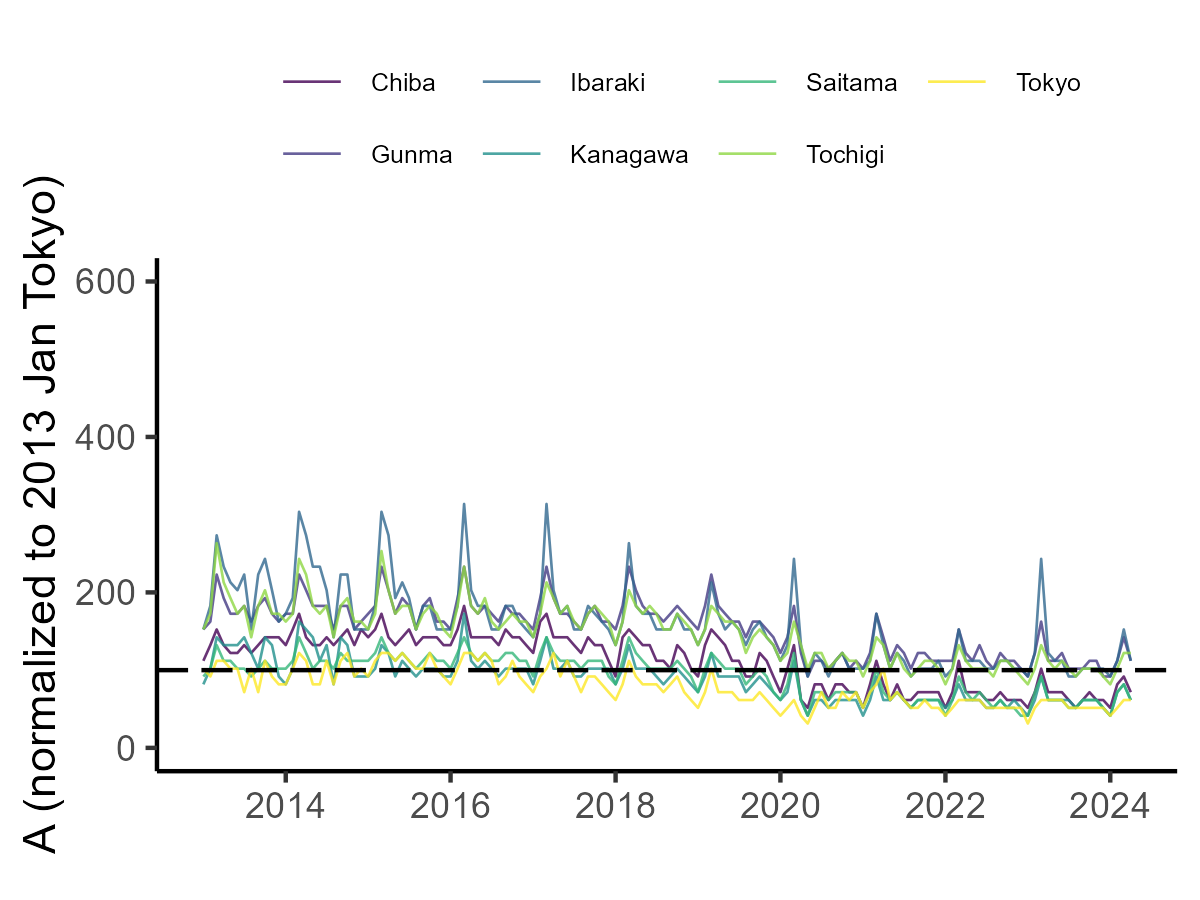
\includegraphics[width = 0.37\textwidth]
  {figuretable/matching_efficiency_month_aggregate_kanto.png}}
  \subfloat[Chubu]{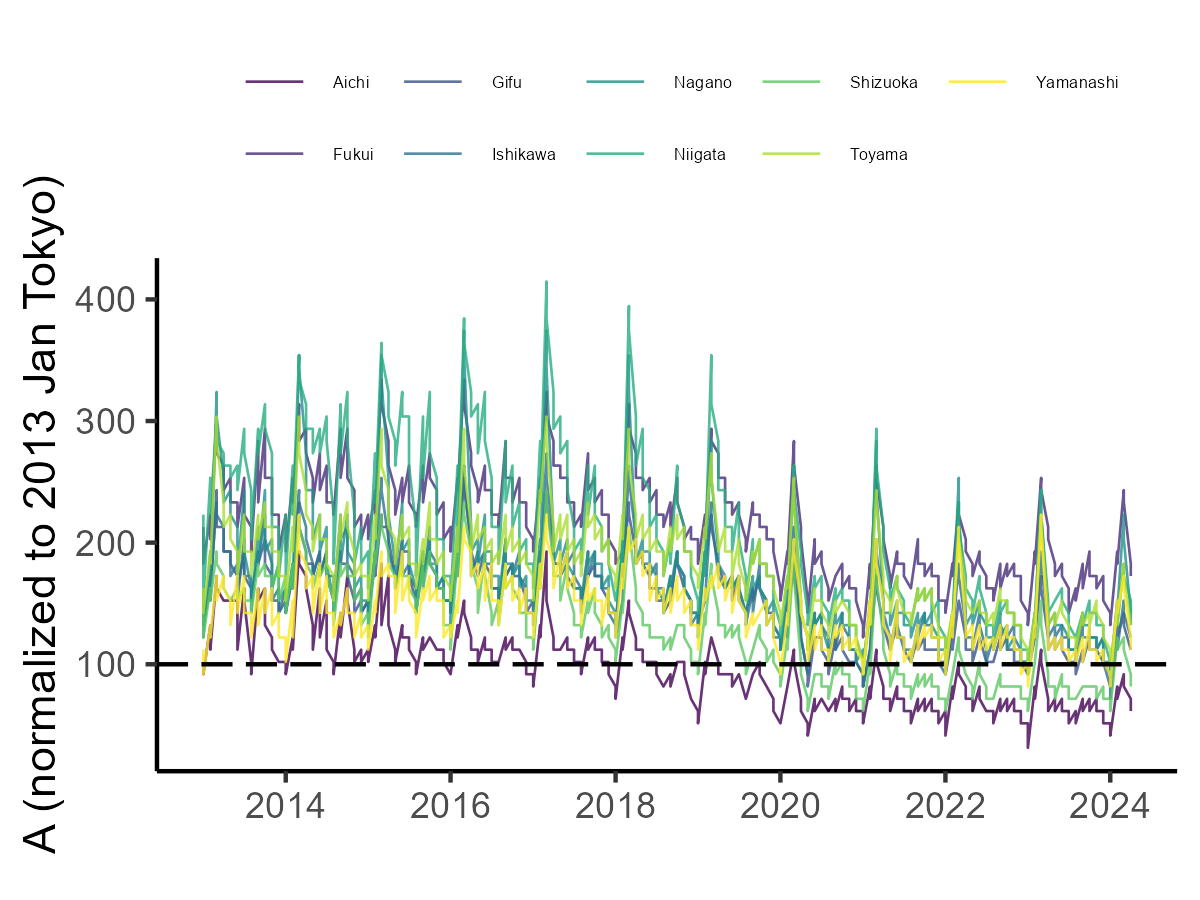
\includegraphics[width = 0.37\textwidth]
  {figuretable/matching_efficiency_month_aggregate_chubu.png}}
  \\
  \subfloat[Kansai]{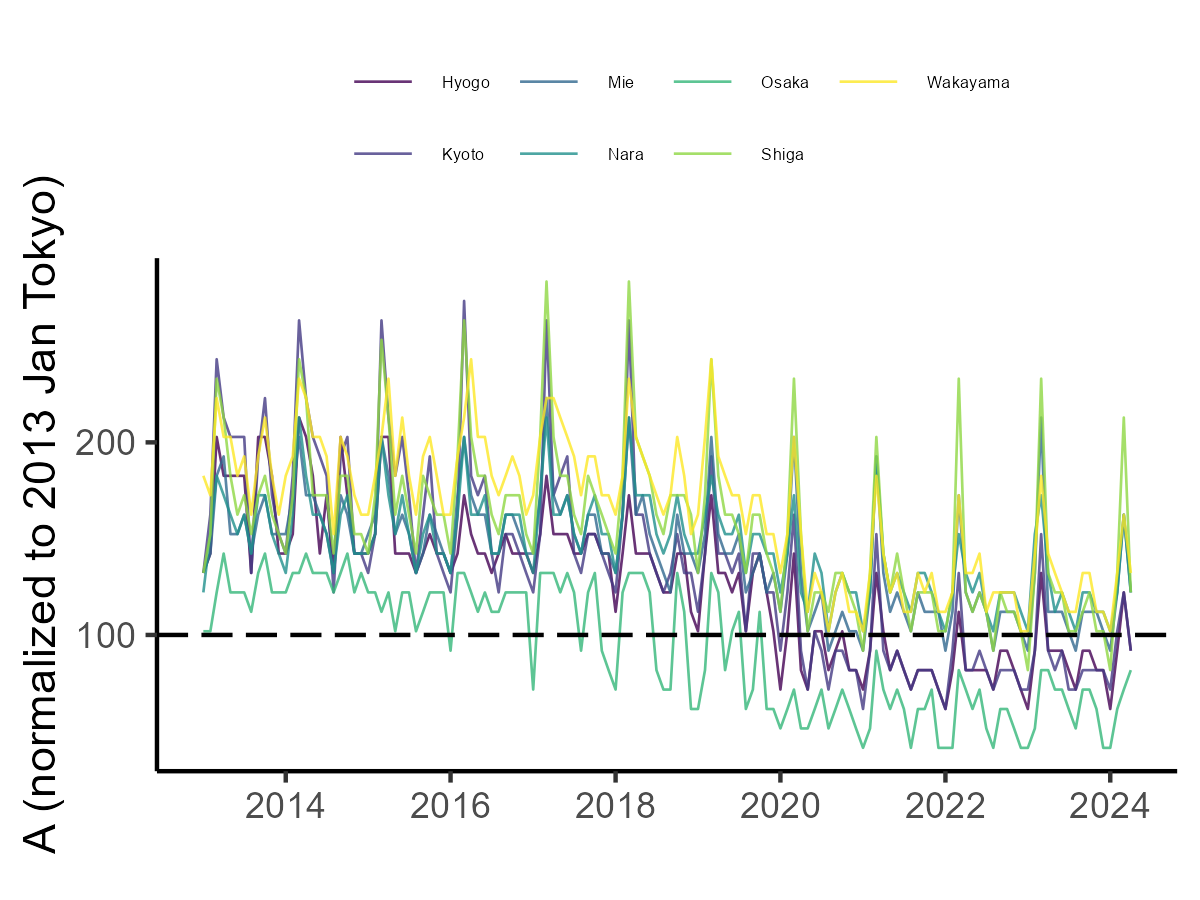
\includegraphics[width = 0.37\textwidth]
  {figuretable/matching_efficiency_month_aggregate_kansai.png}}
  \subfloat[Chugoku]{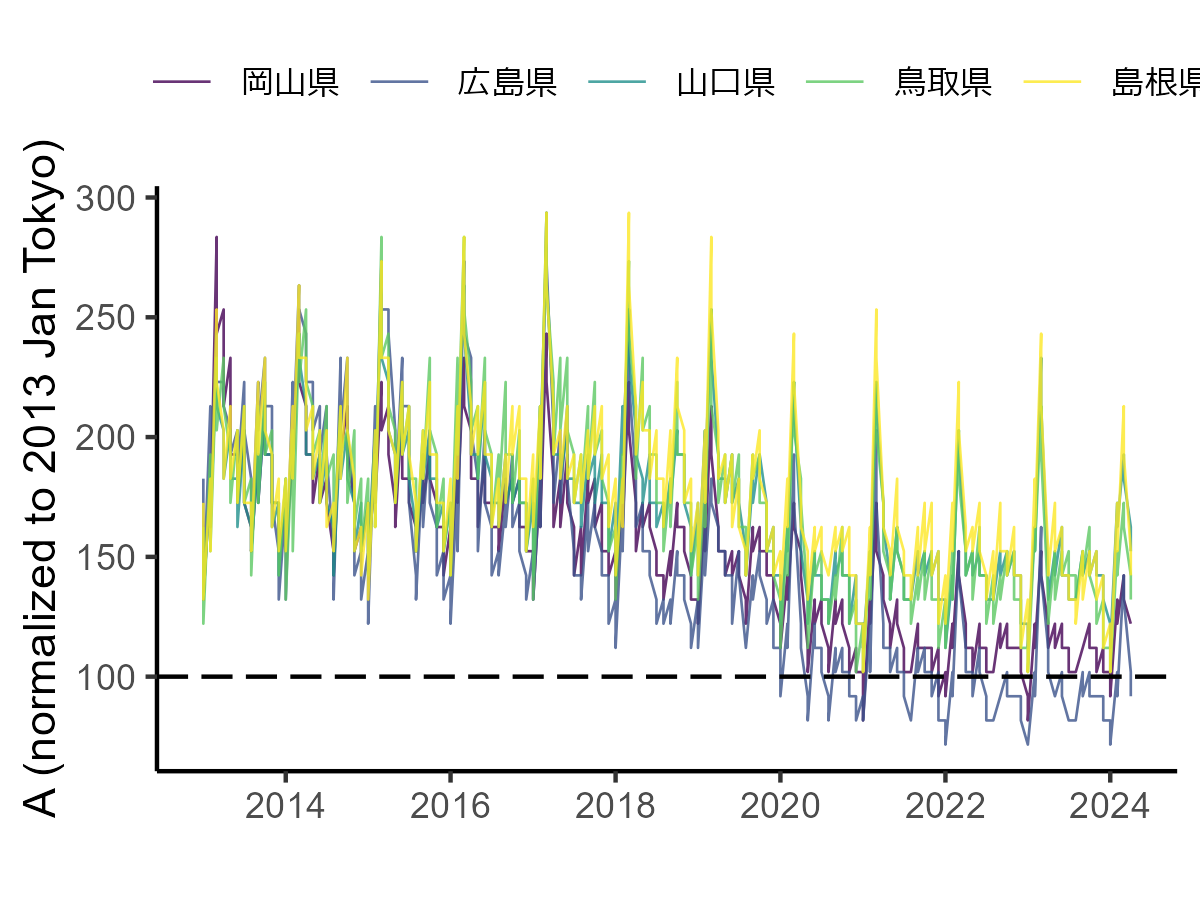
\includegraphics[width = 0.37\textwidth]
  {figuretable/matching_efficiency_month_aggregate_chugoku.png}}\\
  \subfloat[Shikoku]{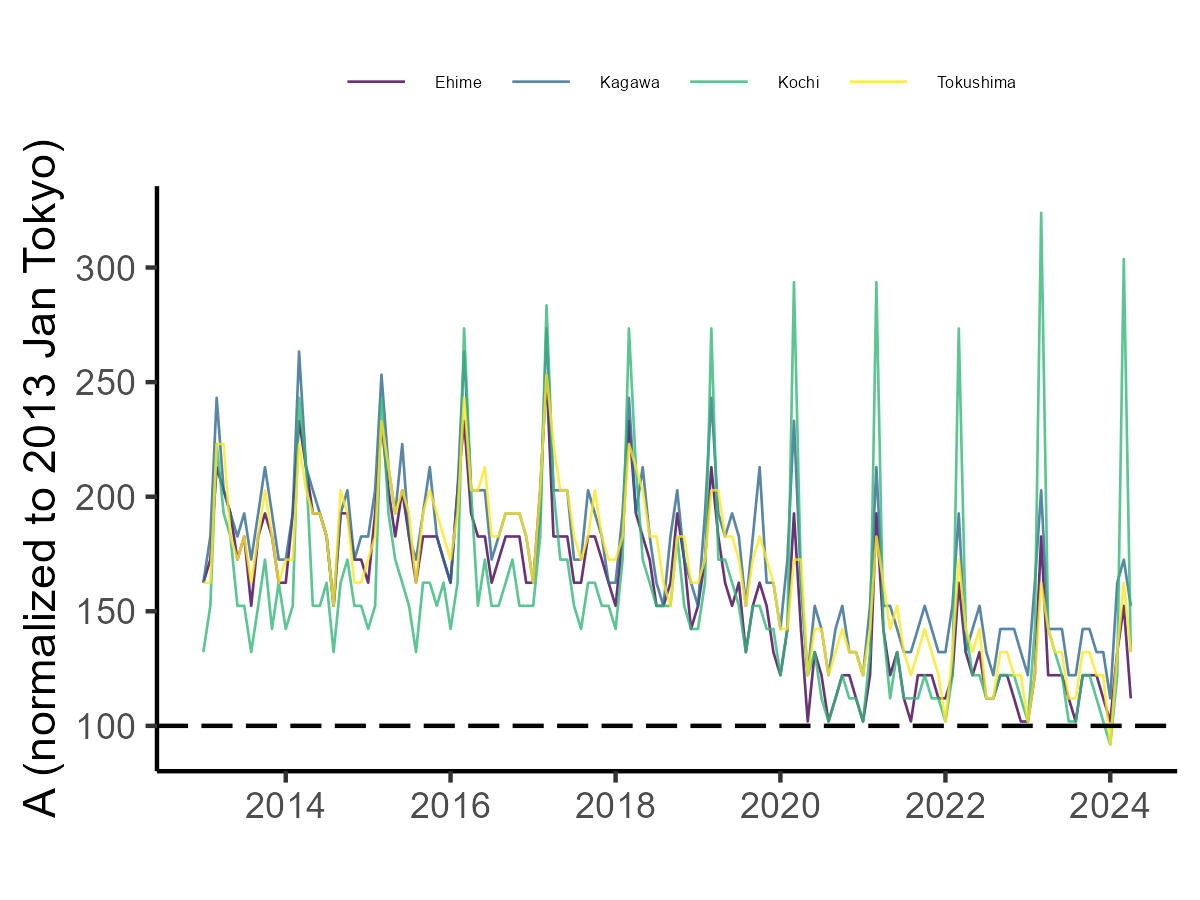
\includegraphics[width = 0.37\textwidth]
  {figuretable/matching_efficiency_month_aggregate_shikoku.png}}
  \subfloat[Kyusyu, Okinawa]{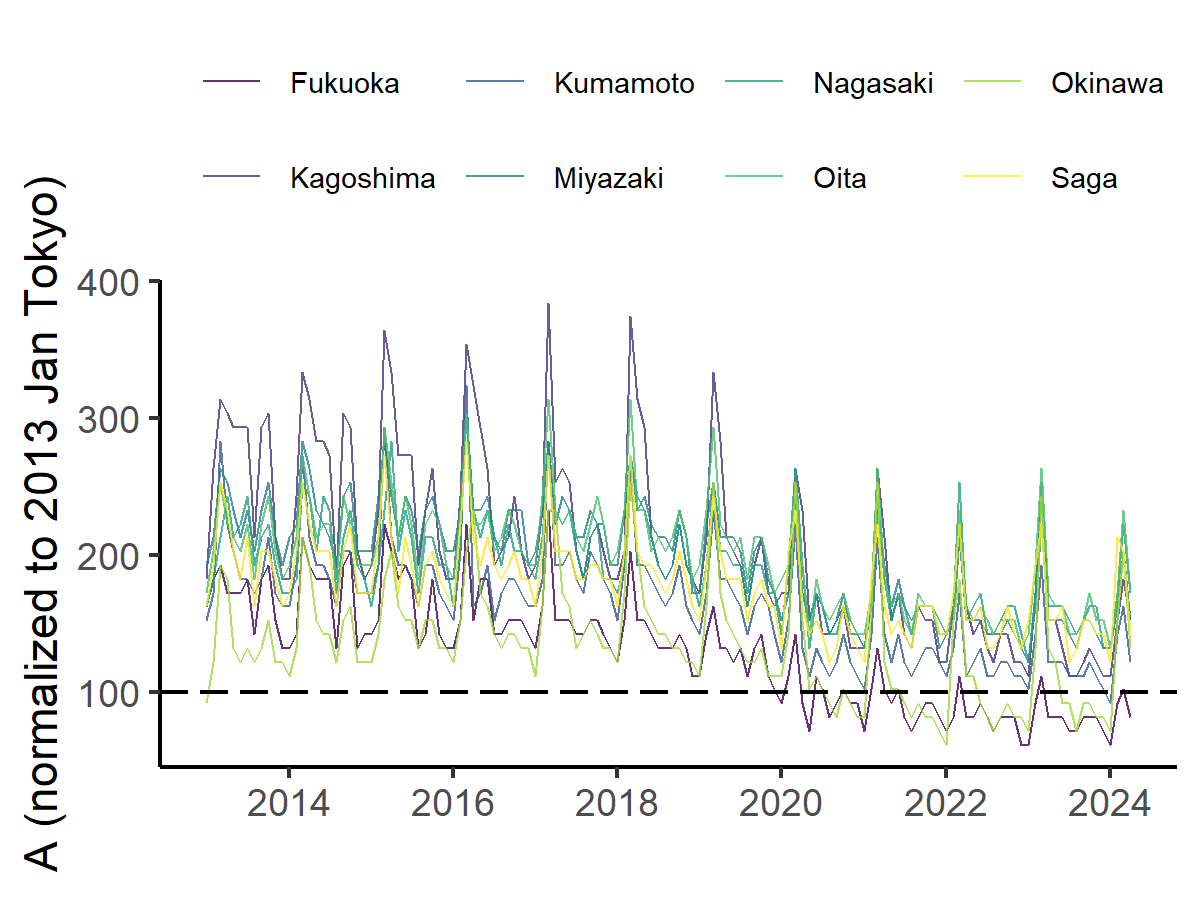
\includegraphics[width = 0.37\textwidth]
  {figuretable/matching_efficiency_month_aggregate_kyushu.png}}
  \caption{Month-level aggregate results 2012-2024}
  \label{fg:month_part_and_full_time_matching_efficiency_prefecture_results} 
  \end{center}
  \footnotesize
  %Note: 
\end{figure} 

Figure \ref{fg:month_part_and_full_time_elasticity_unemployed_month_aggregate_prefecture_results}
\begin{figure}[!ht]
  \begin{center}
  \subfloat[Hokkaido]{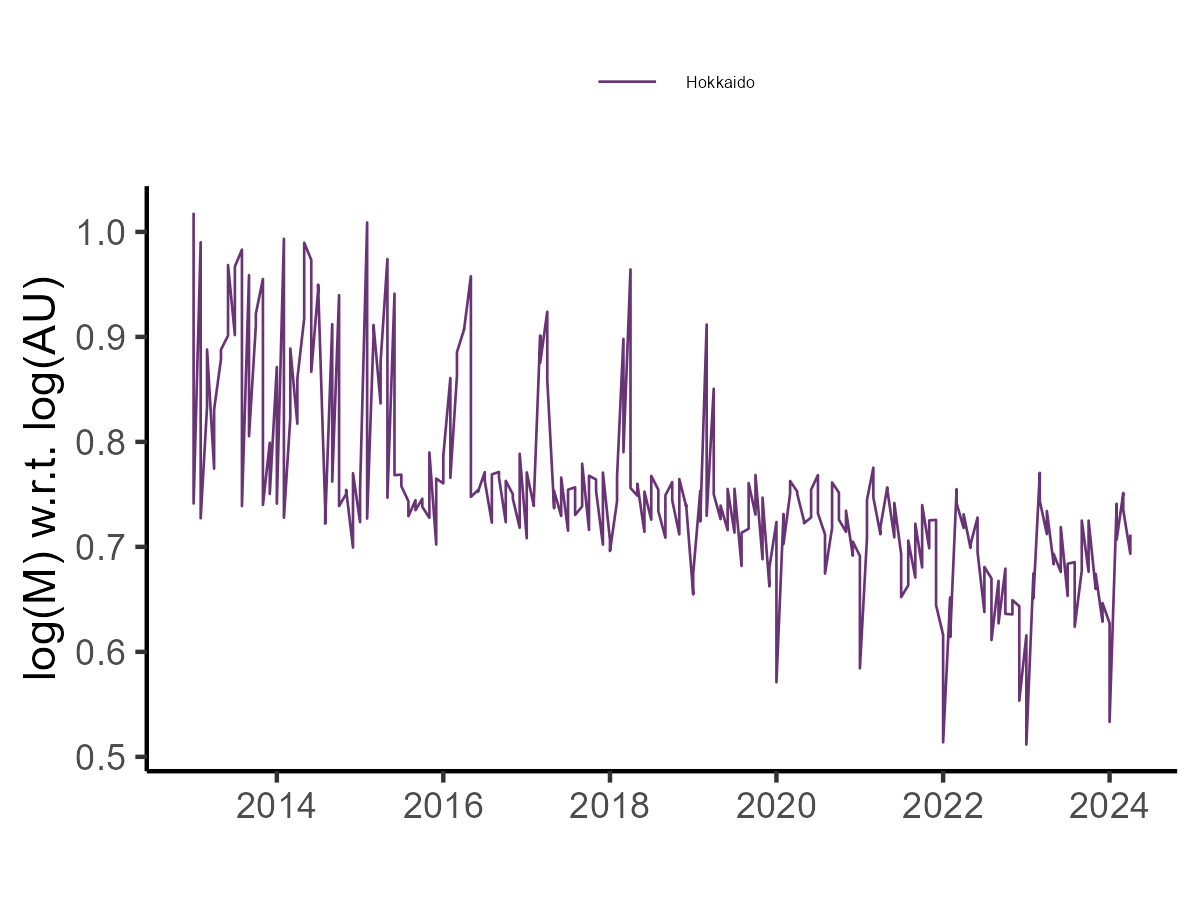
\includegraphics[width = 0.37\textwidth]
  {figuretable/elasticity_unemployed_month_aggregate_hokkaido.png}}
  \subfloat[Tohoku]{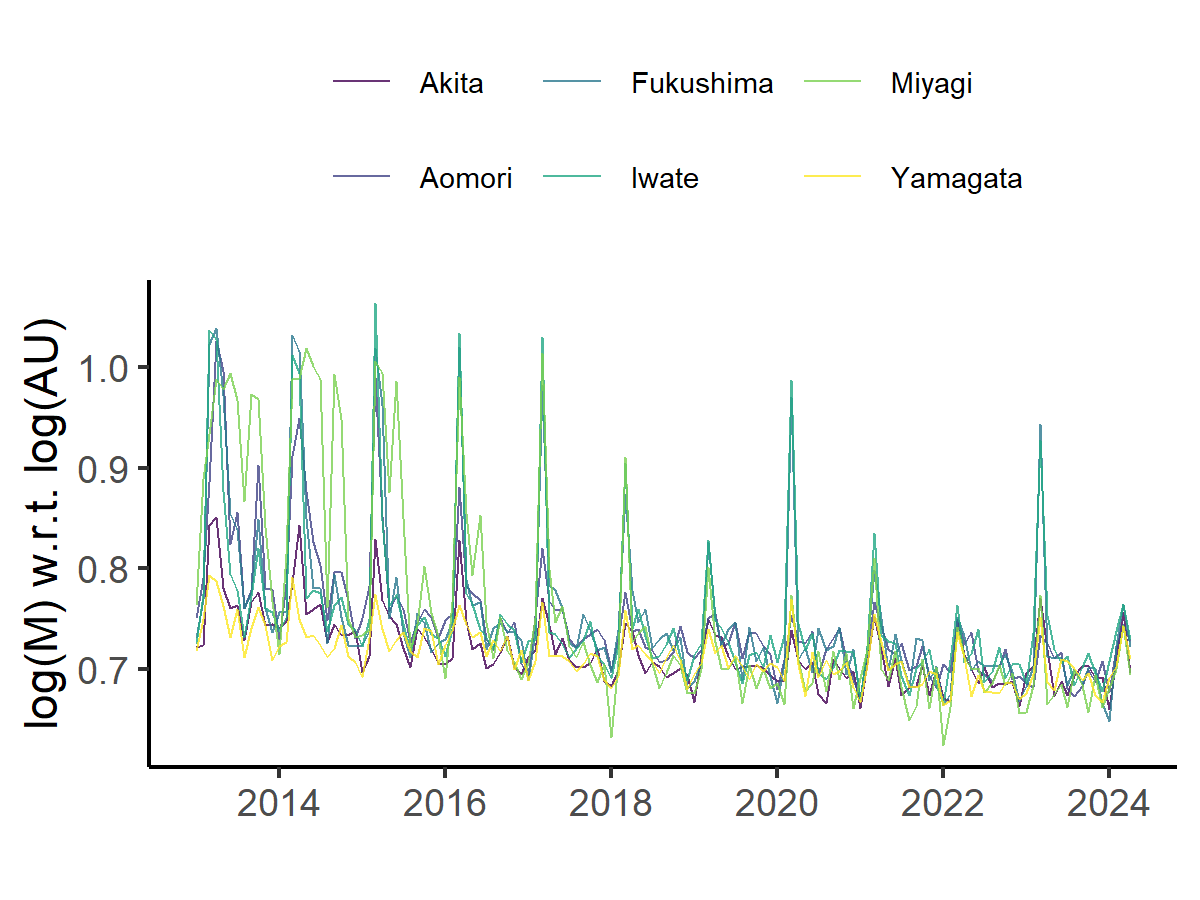
\includegraphics[width = 0.37\textwidth]
  {figuretable/elasticity_unemployed_month_aggregate_tohoku.png}}\\
  \subfloat[Kanto]{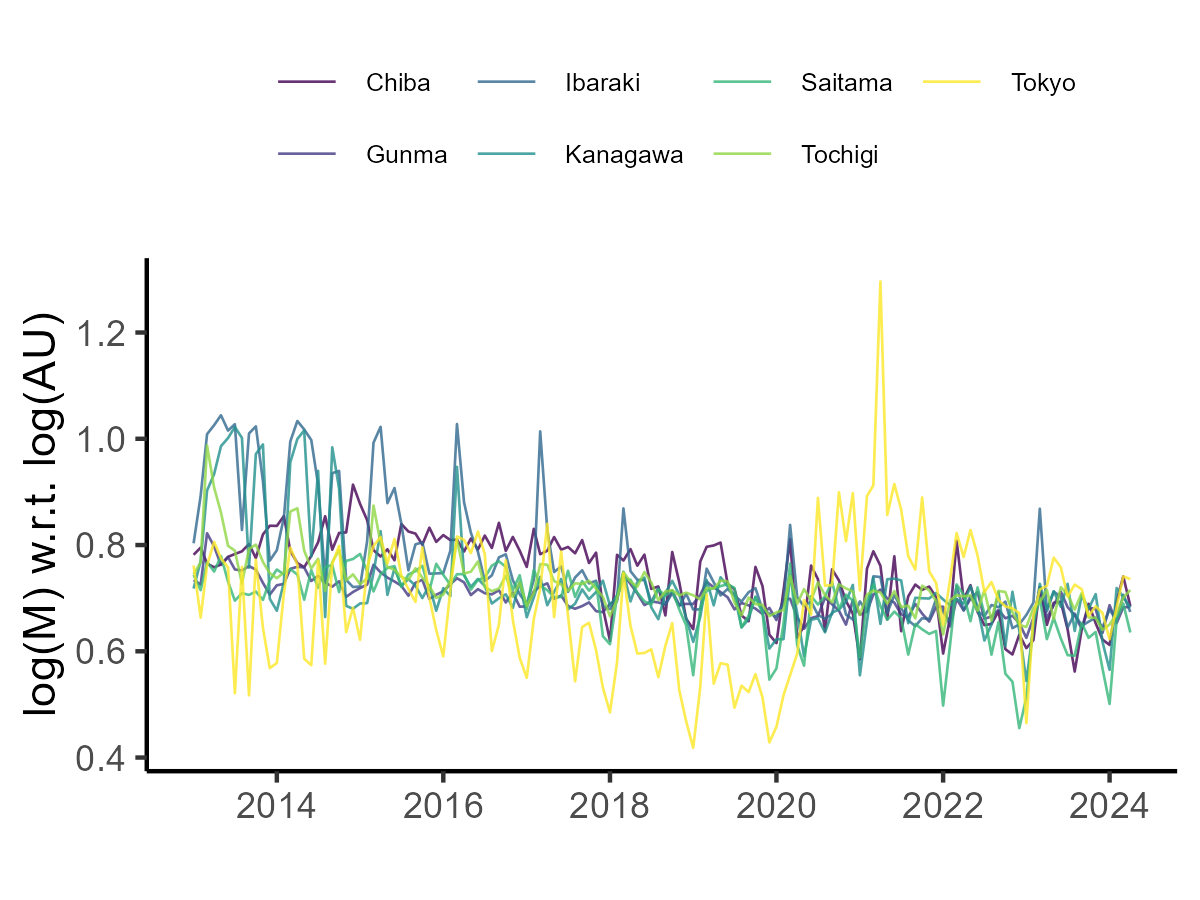
\includegraphics[width = 0.37\textwidth]
  {figuretable/elasticity_unemployed_month_aggregate_kanto.png}}
  \subfloat[Chubu]{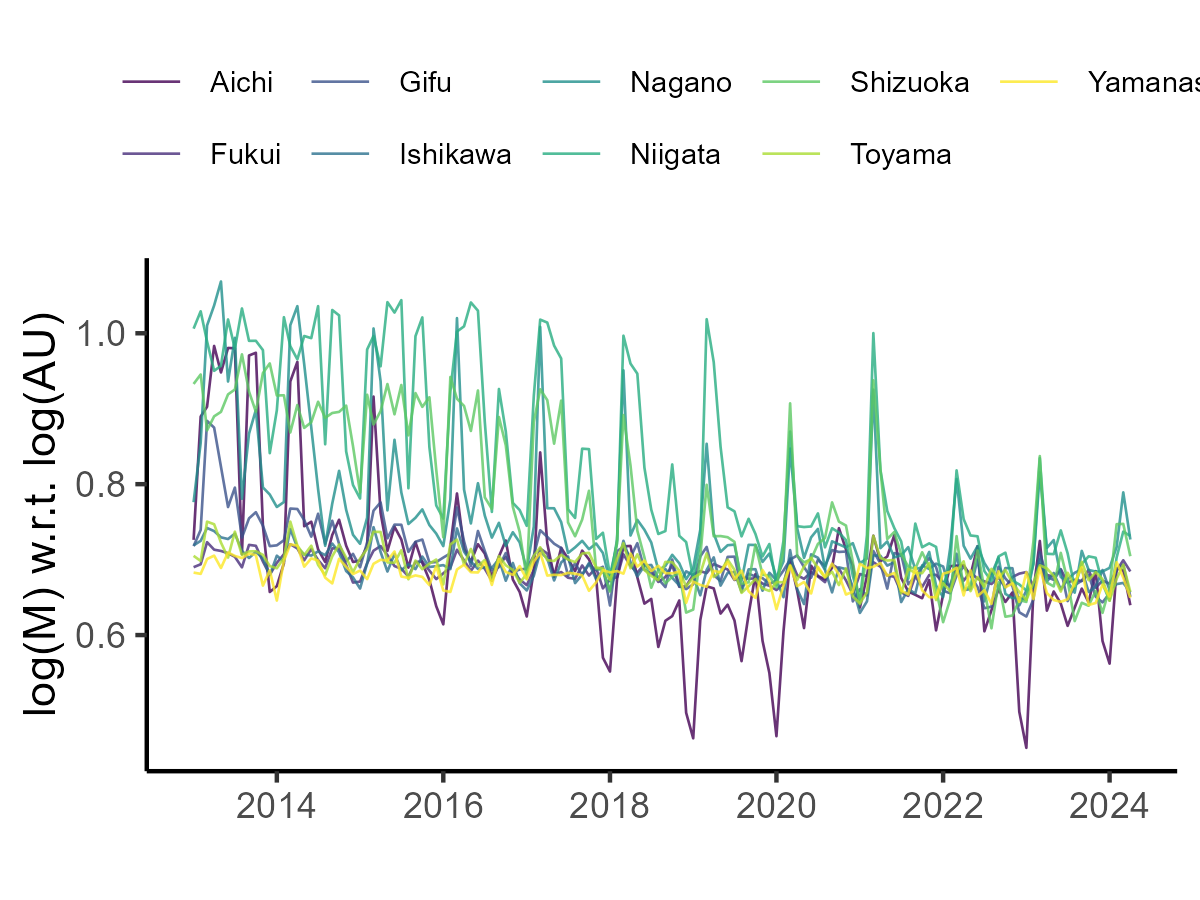
\includegraphics[width = 0.37\textwidth]
  {figuretable/elasticity_unemployed_month_aggregate_chubu.png}}
  \\
  \subfloat[Kansai]{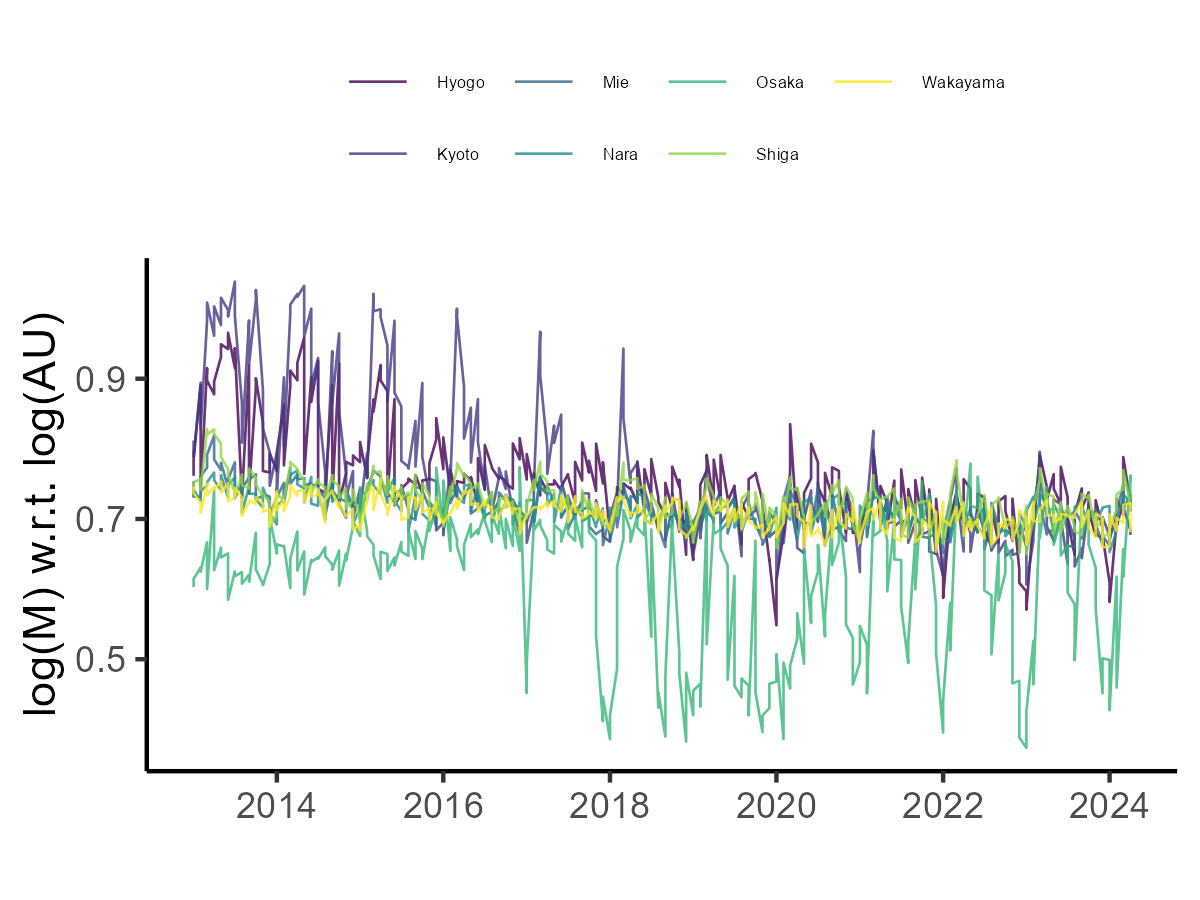
\includegraphics[width = 0.37\textwidth]
  {figuretable/elasticity_unemployed_month_aggregate_kansai.png}}
  \subfloat[Chugoku]{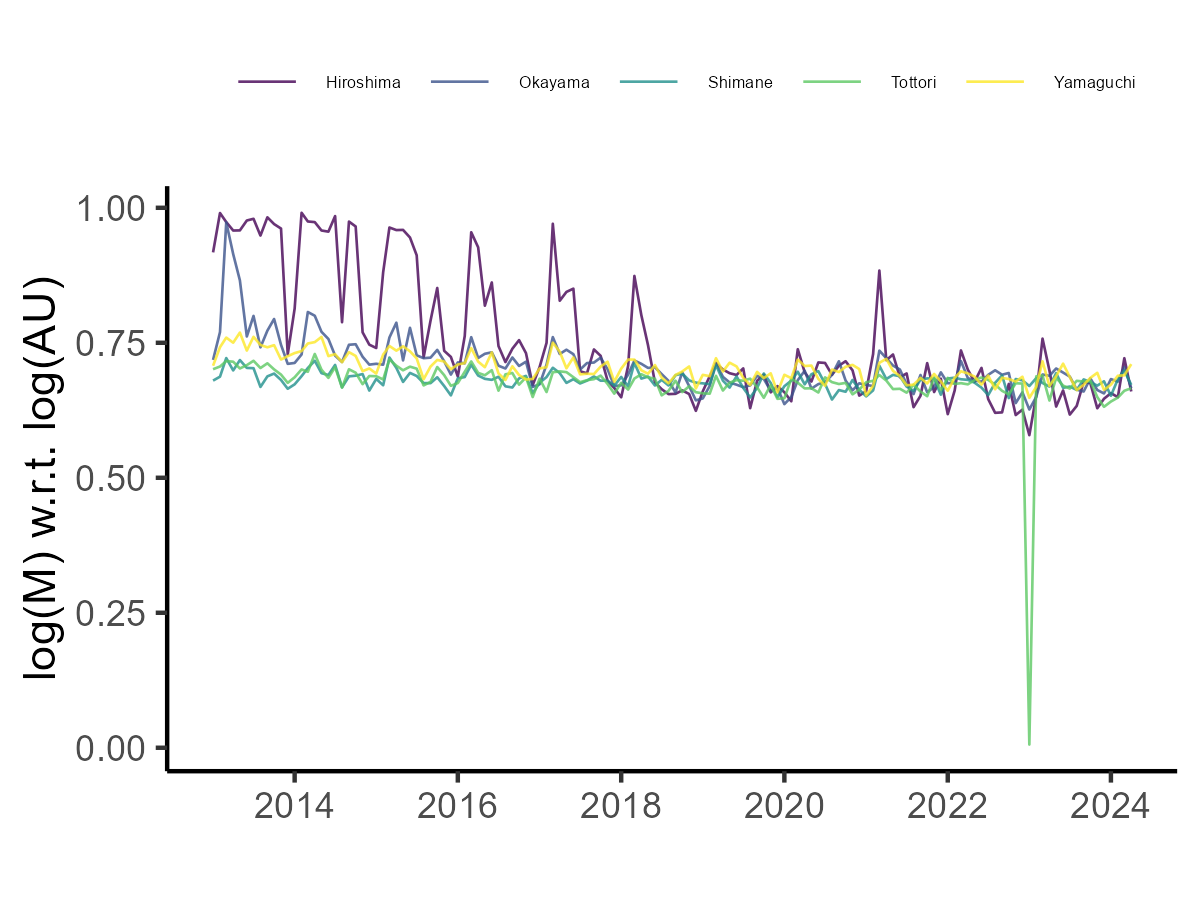
\includegraphics[width = 0.37\textwidth]
  {figuretable/elasticity_unemployed_month_aggregate_chugoku.png}}\\
  \subfloat[Shikoku]{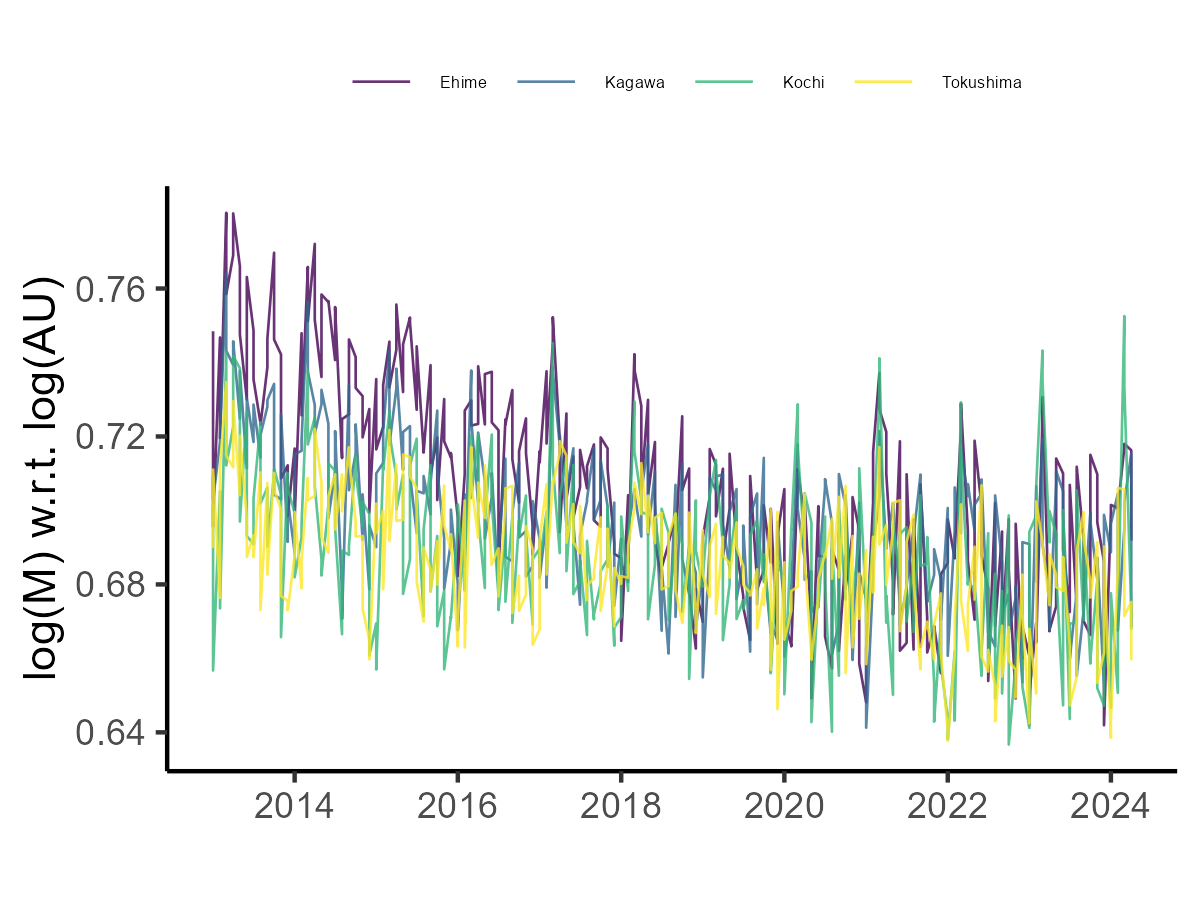
\includegraphics[width = 0.37\textwidth]
  {figuretable/elasticity_unemployed_month_aggregate_shikoku.png}}
  \subfloat[Kyusyu, Okinawa]{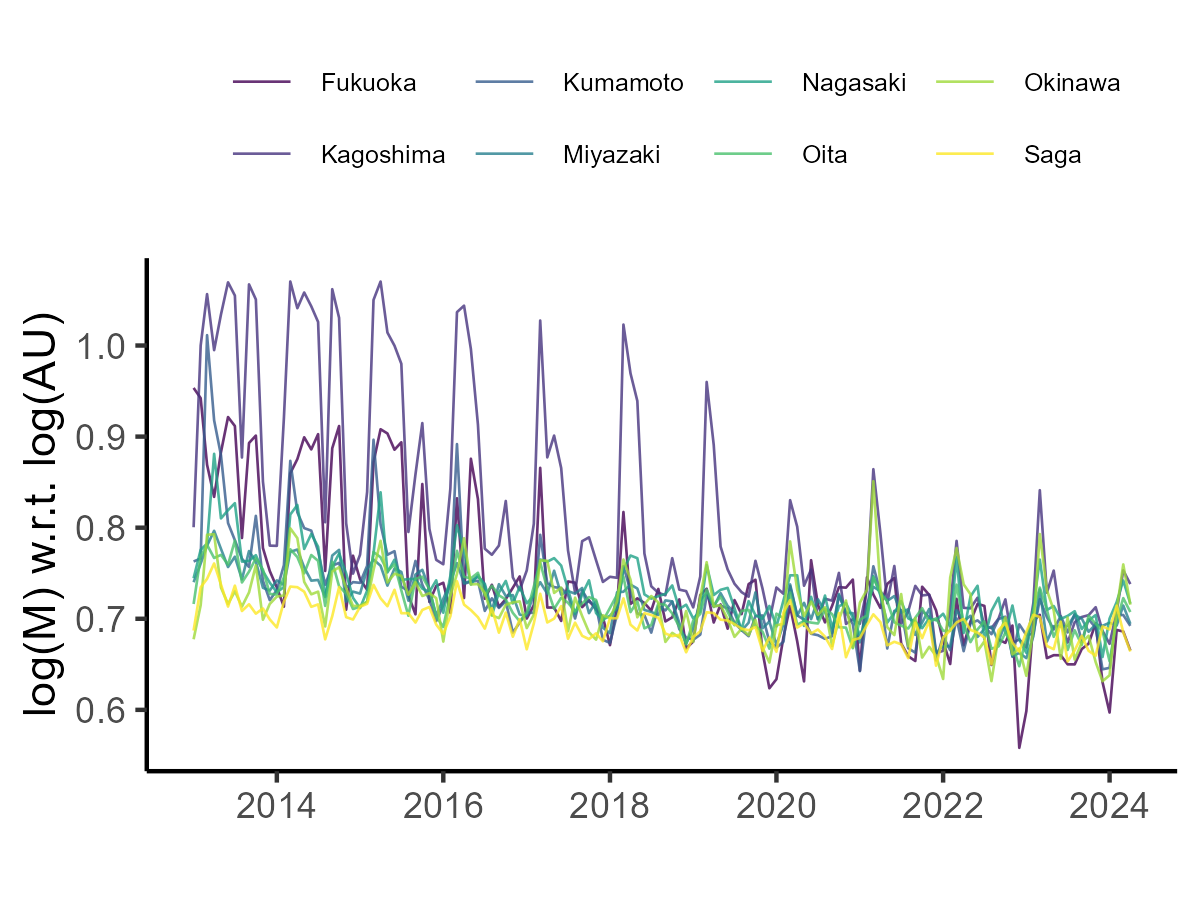
\includegraphics[width = 0.37\textwidth]
  {figuretable/elasticity_unemployed_month_aggregate_kyushu.png}}
  \caption{Month-level aggregate results 2012-2024}
  \label{fg:month_part_and_full_time_elasticity_unemployed_month_aggregate_prefecture_results} 
  \end{center}
  \footnotesize
  %Note: 
\end{figure} 

Figure \ref{fg:month_part_and_full_time_elasticity_vacancy_month_aggregate_prefecture_results}
\begin{figure}[!ht]
  \begin{center}
  \subfloat[Hokkaido]{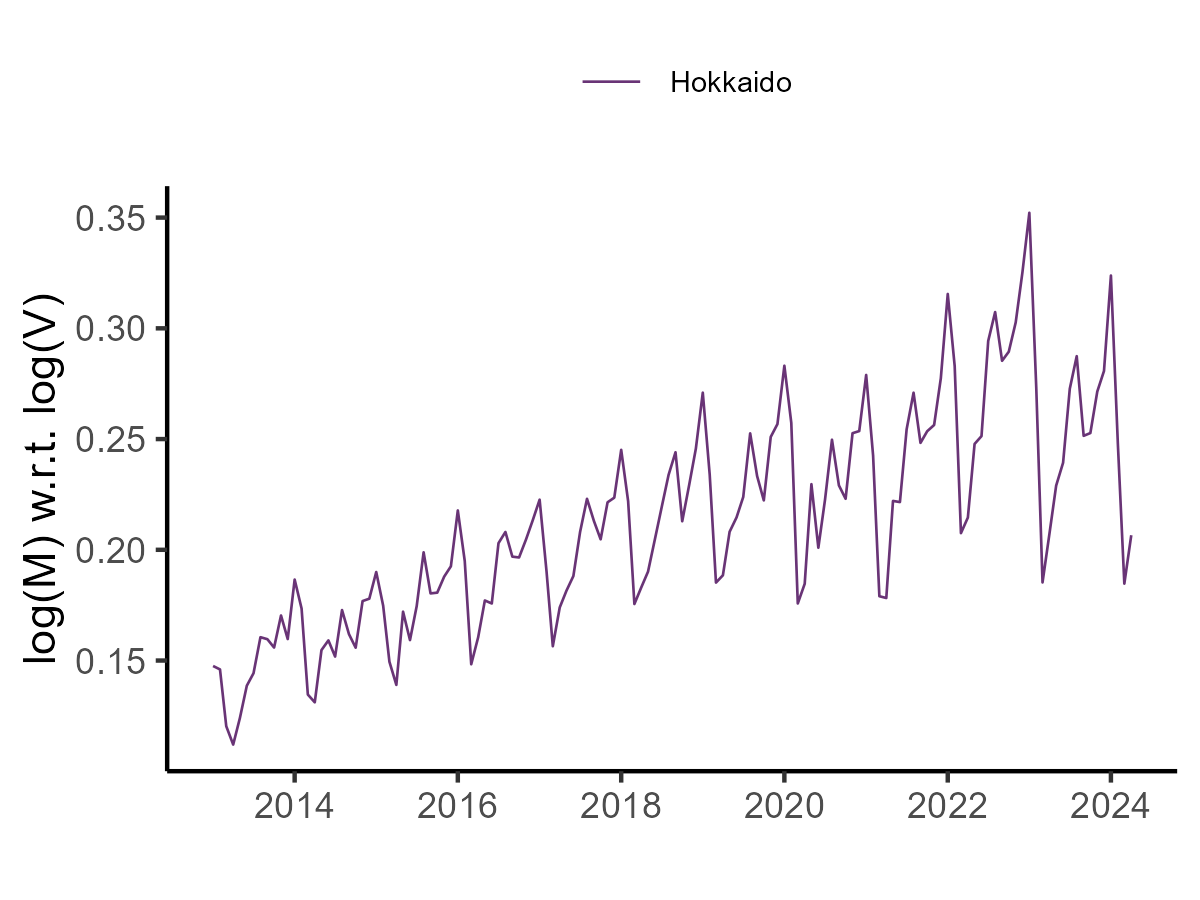
\includegraphics[width = 0.37\textwidth]
  {figuretable/elasticity_vacancy_month_aggregate_hokkaido.png}}
  \subfloat[Tohoku]{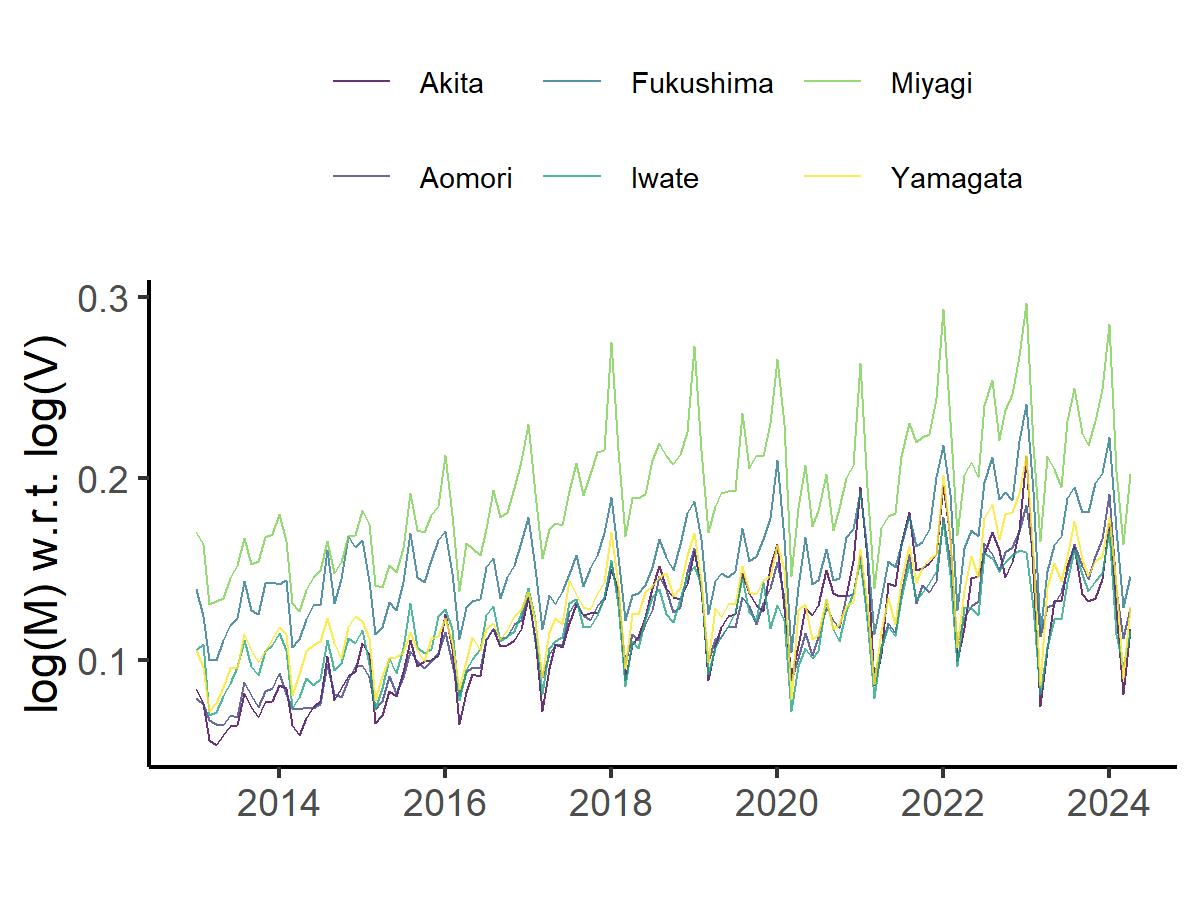
\includegraphics[width = 0.37\textwidth]
  {figuretable/elasticity_vacancy_month_aggregate_tohoku.png}}\\
  \subfloat[Kanto]{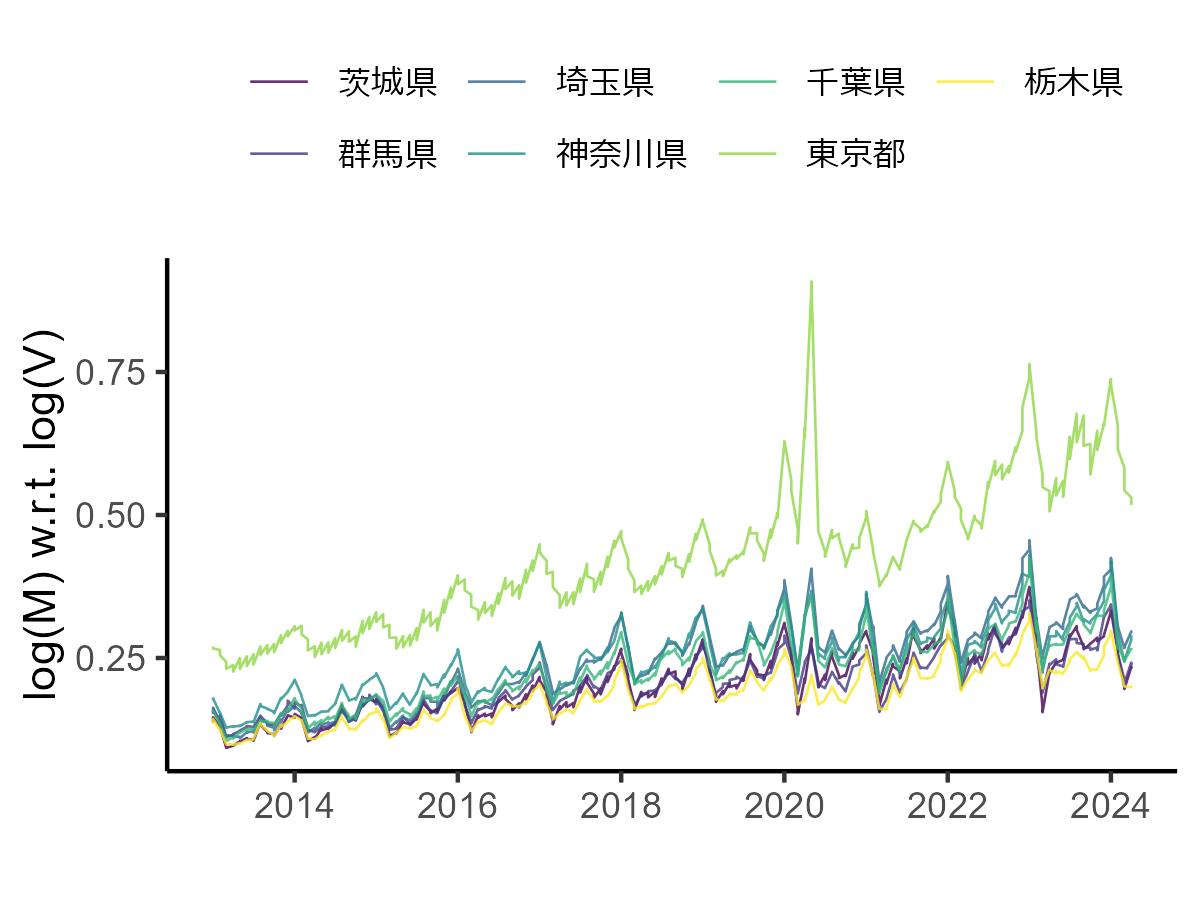
\includegraphics[width = 0.37\textwidth]
  {figuretable/elasticity_vacancy_month_aggregate_kanto.png}}
  \subfloat[Chubu]{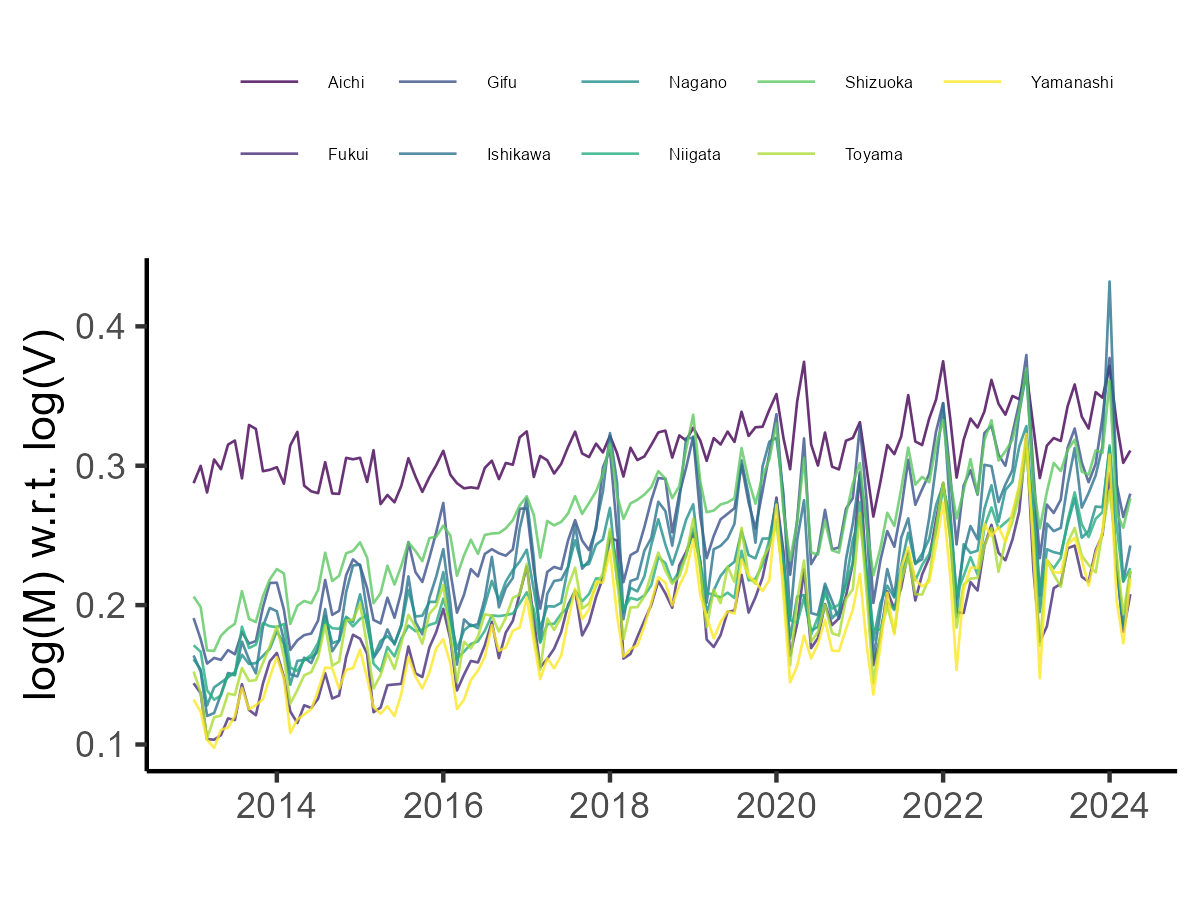
\includegraphics[width = 0.37\textwidth]
  {figuretable/elasticity_vacancy_month_aggregate_chubu.png}}
  \\
  \subfloat[Kansai]{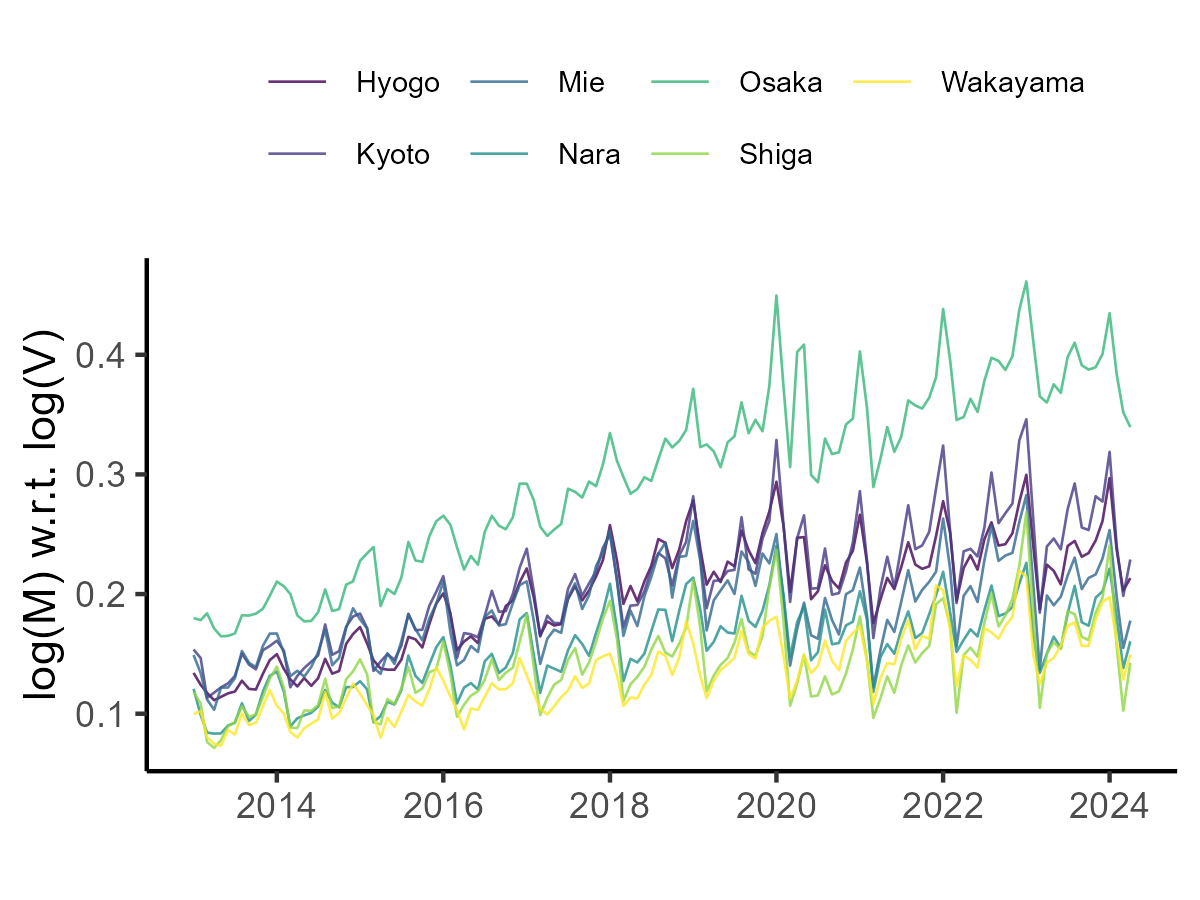
\includegraphics[width = 0.37\textwidth]
  {figuretable/elasticity_vacancy_month_aggregate_kansai.png}}
  \subfloat[Chugoku]{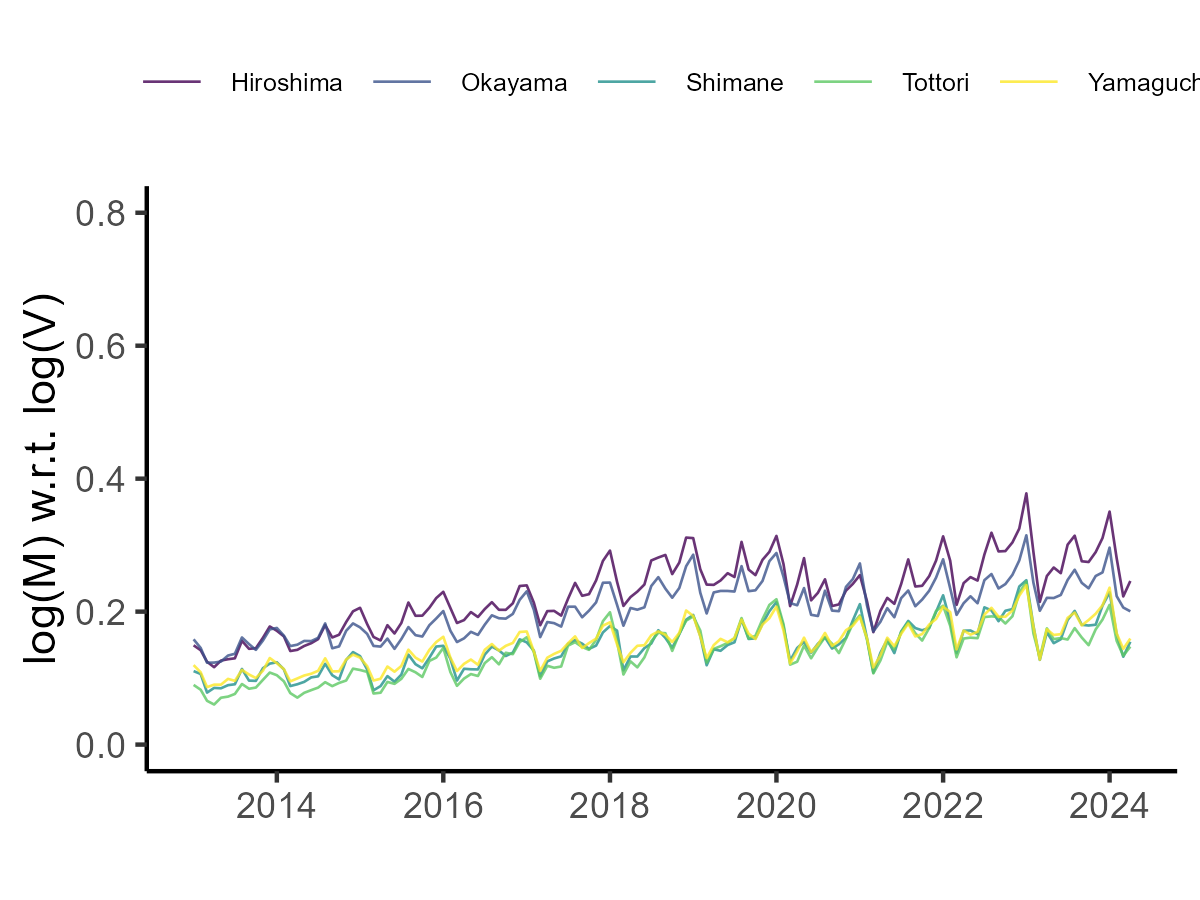
\includegraphics[width = 0.37\textwidth]
  {figuretable/elasticity_vacancy_month_aggregate_chugoku.png}}\\
  \subfloat[Shikoku]{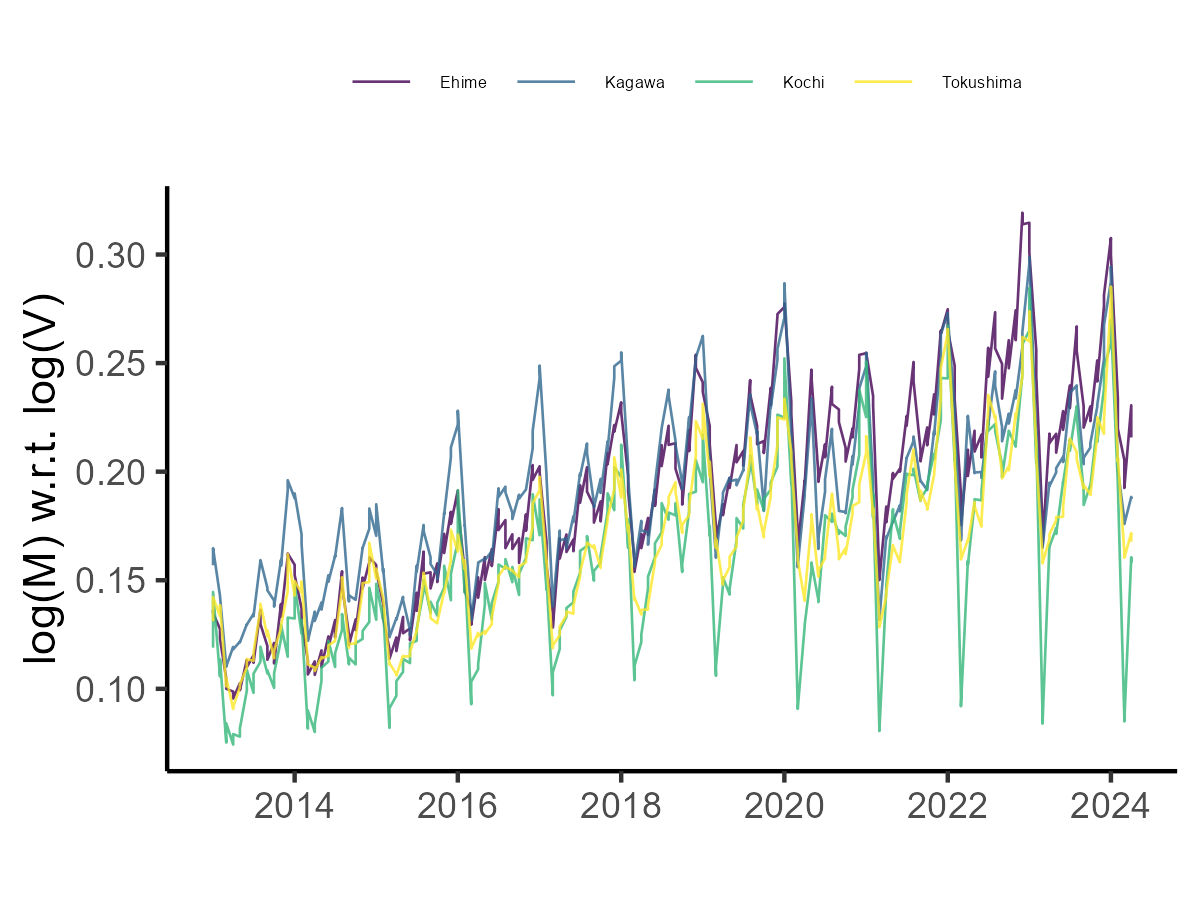
\includegraphics[width = 0.37\textwidth]
  {figuretable/elasticity_vacancy_month_aggregate_shikoku.png}}
  \subfloat[Kyusyu, Okinawa]{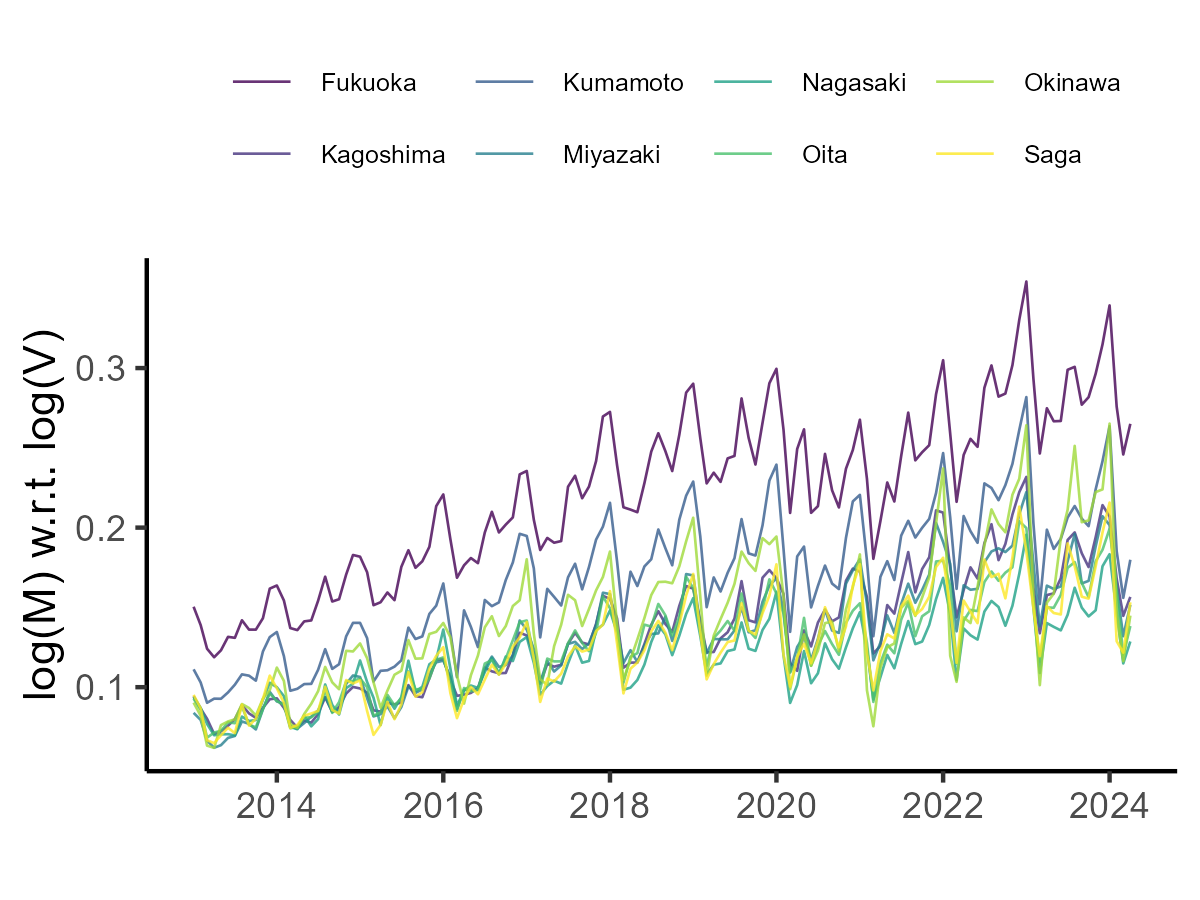
\includegraphics[width = 0.37\textwidth]
  {figuretable/elasticity_vacancy_month_aggregate_kyushu.png}}
  \caption{Month-level aggregate results 2012-2024}
  \label{fg:month_part_and_full_time_elasticity_vacancy_month_aggregate_prefecture_results} 
  \end{center}
  \footnotesize
  %Note: 
\end{figure} 

\begin{itemize}
    \item Full-time and part-time results (Appendix) 6 figures.
    \item \textcolor{blue}{Geographical Mismatch}
\end{itemize}

\subsection{Job category level results in 2012-2024}

Figure \ref{fg:month_part_and_full_time_matching_efficiency_job_category_results}


\begin{figure}[!ht]
  \begin{center}
  \subfloat[managerial]{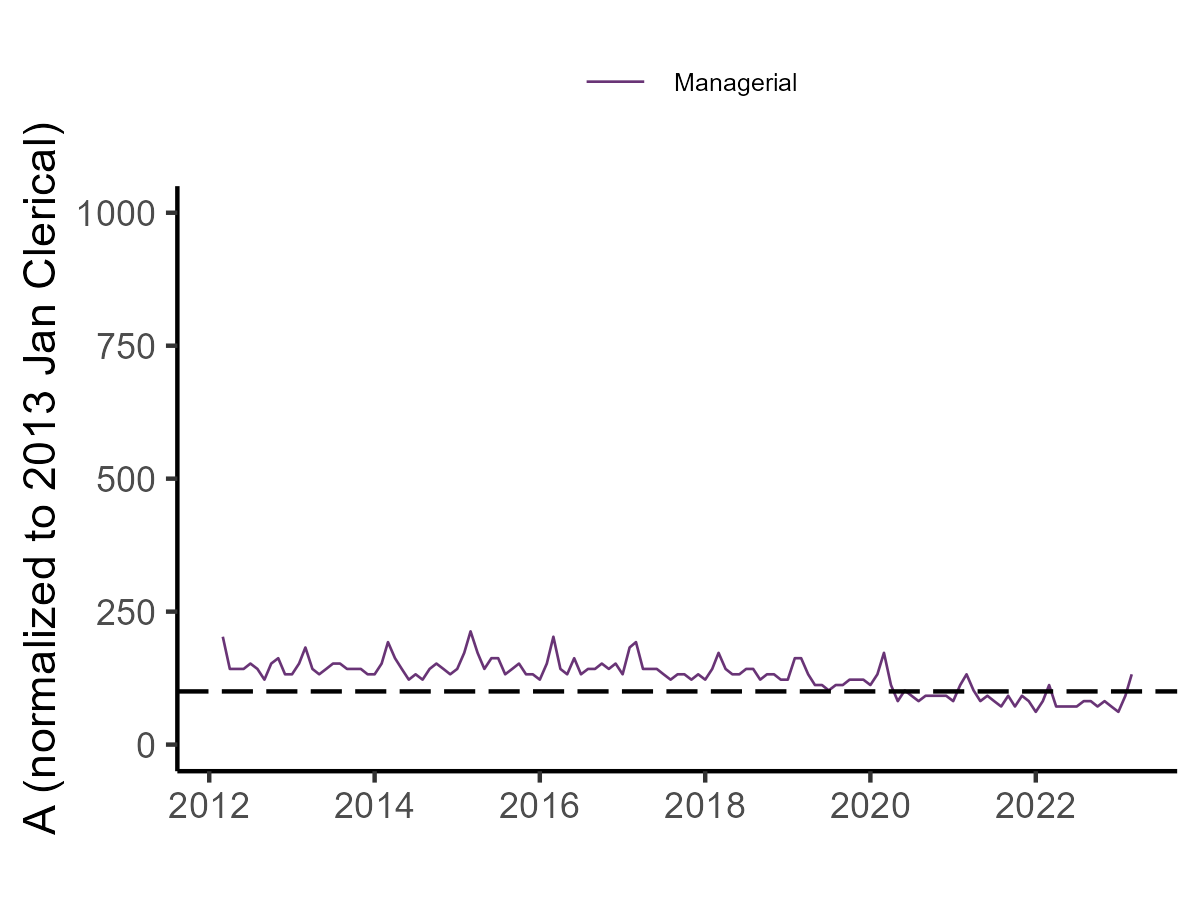
\includegraphics[width = 0.30\textwidth]
  {figuretable/matching_efficiency_month_aggregate_managerial.png}}
  \subfloat[professional and technical]{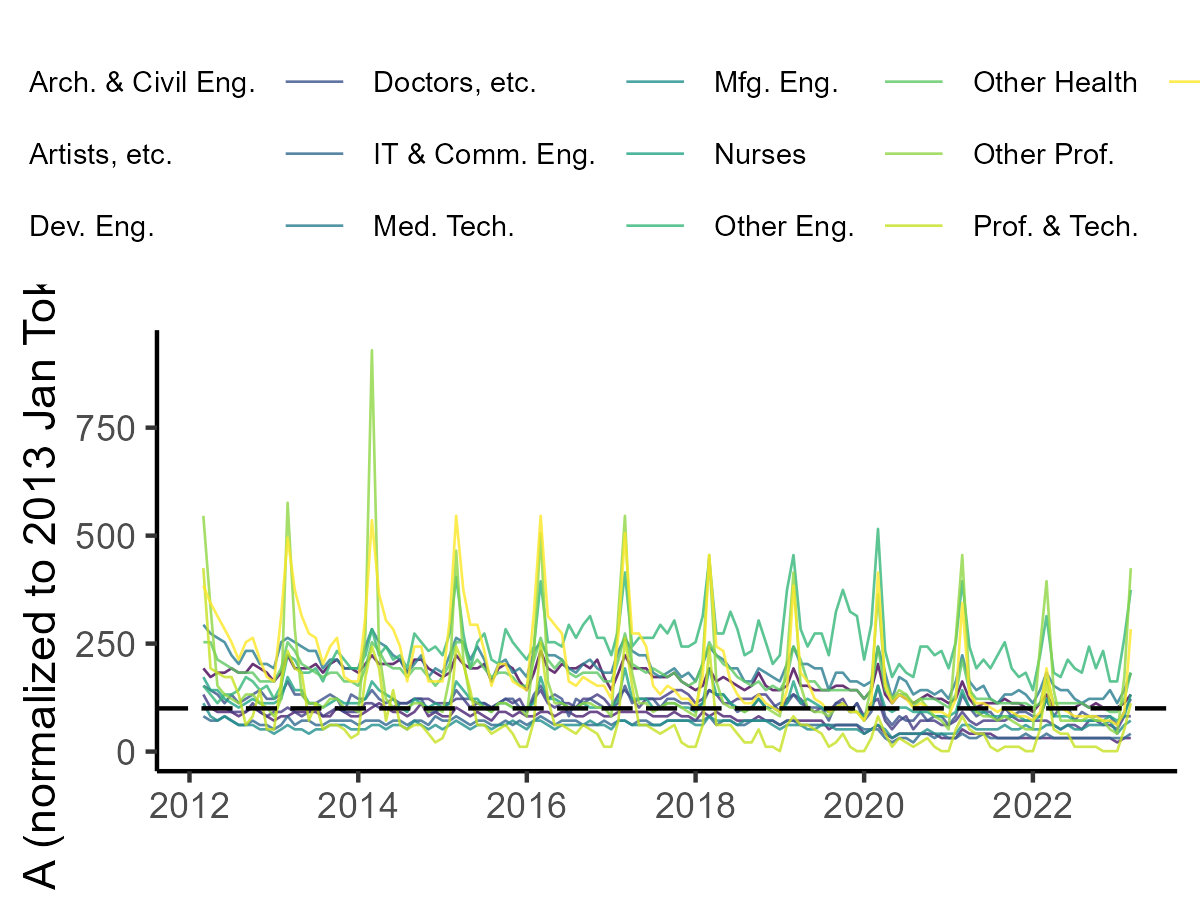
\includegraphics[width = 0.30\textwidth]
  {figuretable/matching_efficiency_month_aggregate_professional_and_technical.png}}
  \subfloat[clerical]{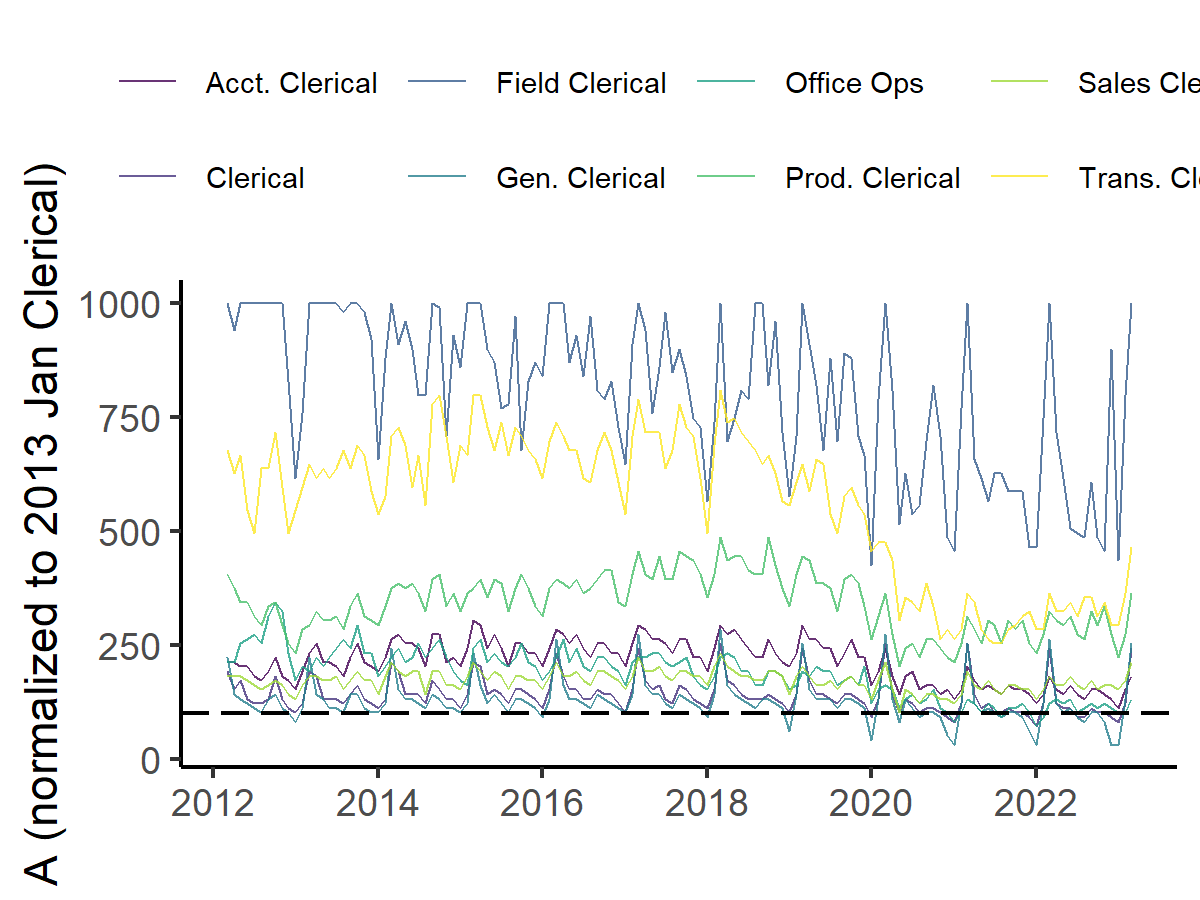
\includegraphics[width = 0.30\textwidth]
  {figuretable/matching_efficiency_month_aggregate_clerical.png}}\\
  \subfloat[sales]{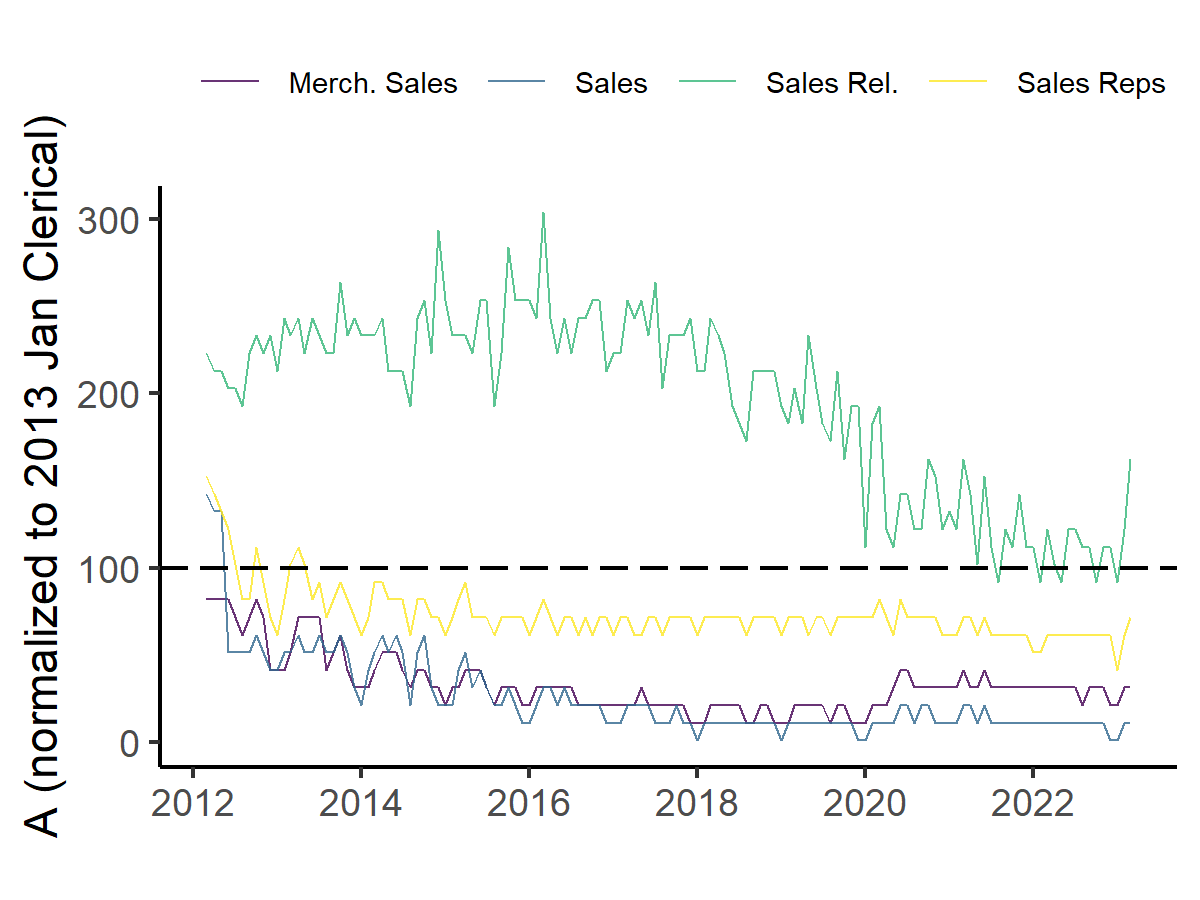
\includegraphics[width = 0.30\textwidth]
  {figuretable/matching_efficiency_month_aggregate_sales.png}}
  \subfloat[service]{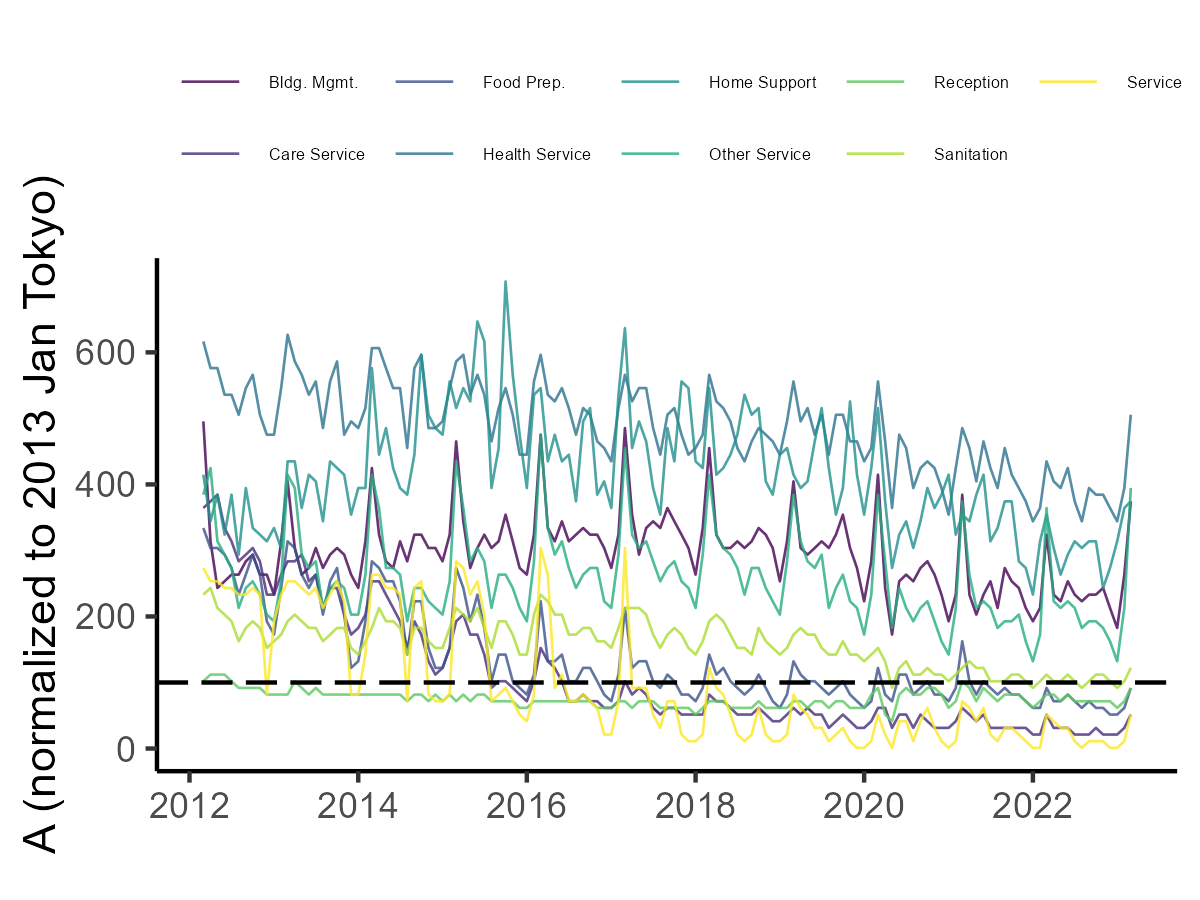
\includegraphics[width = 0.30\textwidth]
  {figuretable/matching_efficiency_month_aggregate_service.png}}
  \subfloat[agriculture forestry and fishing]{\includegraphics[width = 0.30\textwidth]
  {figuretable/matching_efficiency_month_aggregate_agriculture_forestry_and_fishing.png}}\\
  \subfloat[production]{\includegraphics[width = 0.30\textwidth]
  {figuretable/matching_efficiency_month_aggregate_production.png}}
  \subfloat[transportation and machine operation]{\includegraphics[width = 0.30\textwidth]
  {figuretable/matching_efficiency_month_aggregate_transportation_and_machine_operation.png}}
  \subfloat[construction and mining]{\includegraphics[width = 0.30\textwidth]
  {figuretable/matching_efficiency_month_aggregate_construction_and_mining.png}}\\
  \subfloat[transportation cleaning and packaging]{\includegraphics[width = 0.30\textwidth]
  {figuretable/matching_efficiency_month_aggregate_transportation_cleaning_and_packaging.png}}
  \subfloat[security]{\includegraphics[width = 0.30\textwidth]
  {figuretable/matching_efficiency_month_aggregate_security.png}}
  \caption{Month-level aggregate results 2012-2024}
  \label{fg:month_part_and_full_time_matching_efficiency_job_category_results} 
  \end{center}
  \footnotesize
  %Note: 
\end{figure} 

Figure \ref{fg:month_part_and_full_time_elasticity_unemployed_month_aggregate_job_category_results}
\begin{figure}[!ht]
  \begin{center}
  \subfloat[managerial]{\includegraphics[width = 0.30\textwidth]
  {figuretable/elasticity_unemployed_month_aggregate_managerial.png}}
  \subfloat[professional and technical]{\includegraphics[width = 0.30\textwidth]
  {figuretable/elasticity_unemployed_month_aggregate_professional_and_technical.png}}
  \subfloat[clerical]{\includegraphics[width = 0.30\textwidth]
  {figuretable/elasticity_unemployed_month_aggregate_clerical.png}}\\
  \subfloat[sales]{\includegraphics[width = 0.30\textwidth]
  {figuretable/elasticity_unemployed_month_aggregate_sales.png}}
  \subfloat[service]{\includegraphics[width = 0.30\textwidth]
  {figuretable/elasticity_unemployed_month_aggregate_service.png}}
  \subfloat[agriculture forestry and fishing]{\includegraphics[width = 0.30\textwidth]
  {figuretable/elasticity_unemployed_month_aggregate_agriculture_forestry_and_fishing.png}}\\
  \subfloat[production]{\includegraphics[width = 0.30\textwidth]
  {figuretable/elasticity_unemployed_month_aggregate_production.png}}
  \subfloat[transportation and machine operation]{\includegraphics[width = 0.30\textwidth]
  {figuretable/elasticity_unemployed_month_aggregate_transportation_and_machine_operation.png}}
  \subfloat[construction and mining]{\includegraphics[width = 0.30\textwidth]
  {figuretable/elasticity_unemployed_month_aggregate_construction_and_mining.png}}\\
  \subfloat[transportation cleaning and packaging]{\includegraphics[width = 0.30\textwidth]
  {figuretable/elasticity_unemployed_month_aggregate_transportation_cleaning_and_packaging.png}}
  \subfloat[security]{\includegraphics[width = 0.30\textwidth]
  {figuretable/elasticity_unemployed_month_aggregate_security.png}}
  \caption{Month-level aggregate results 2012-2024}
  \label{fg:month_part_and_full_time_elasticity_unemployed_month_aggregate_job_category_results} 
  \end{center}
  \footnotesize
  %Note: 
\end{figure} 

Figure \ref{fg:month_part_and_full_time_elasticity_vacancy_month_aggregate_job_category_results}
\begin{figure}[!ht]
  \begin{center}
  \subfloat[managerial]{\includegraphics[width = 0.30\textwidth]
  {figuretable/elasticity_vacancy_month_aggregate_managerial.png}}
  \subfloat[professional and technical]{\includegraphics[width = 0.30\textwidth]
  {figuretable/elasticity_vacancy_month_aggregate_professional_and_technical.png}}
  \subfloat[clerical]{\includegraphics[width = 0.30\textwidth]
  {figuretable/elasticity_vacancy_month_aggregate_clerical.png}}\\
  \subfloat[sales]{\includegraphics[width = 0.30\textwidth]
  {figuretable/elasticity_vacancy_month_aggregate_sales.png}}
  \subfloat[service]{\includegraphics[width = 0.30\textwidth]
  {figuretable/elasticity_vacancy_month_aggregate_service.png}}
  \subfloat[agriculture forestry and fishing]{\includegraphics[width = 0.30\textwidth]
  {figuretable/elasticity_vacancy_month_aggregate_agriculture_forestry_and_fishing.png}}\\
  \subfloat[production]{\includegraphics[width = 0.30\textwidth]
  {figuretable/elasticity_vacancy_month_aggregate_production.png}}
  \subfloat[transportation and machine operation]{\includegraphics[width = 0.30\textwidth]
  {figuretable/elasticity_vacancy_month_aggregate_transportation_and_machine_operation.png}}
  \subfloat[construction and mining]{\includegraphics[width = 0.30\textwidth]
  {figuretable/elasticity_vacancy_month_aggregate_construction_and_mining.png}}\\
  \subfloat[transportation cleaning and packaging]{\includegraphics[width = 0.30\textwidth]
  {figuretable/elasticity_vacancy_month_aggregate_transportation_cleaning_and_packaging.png}}
  \subfloat[security]{\includegraphics[width = 0.30\textwidth]
  {figuretable/elasticity_vacancy_month_aggregate_security.png}}
  \caption{Month-level aggregate results 2012-2024}
  \label{fg:month_part_and_full_time_elasticity_vacancy_month_aggregate_job_category_results} 
  \end{center}
  \footnotesize
  %Note: 
\end{figure} 

\begin{itemize}
    \item Full-time and part-time results (Appendix) 6 figures.
    \item \textcolor{blue}{Occupational Category Mismatch}
\end{itemize}





\section{Conclusion}

I investigate how matching efficiency in the labor market via Public Employment Security Offices in Japan for unemployed workers changed during the period 1972-2024. By applying a novel nonparametric identification approach proposed by \cite{lange2020beyond} to monthly data, I find that matching efficiency (normalized to 1972) exhibits a declining trend with notable fluctuations, consistent with the downward trends in job and worker finding rates. \textcolor{blue}{[TBA] Geographical mismatch results.} Finally, I highlight that comparing matching elasticity with respect to the number of unemployed workers across different datasets is challenging due to differences in scale normalization.


\paragraph{Acknowledgments}
I thank Fuhito Kojima, Kosuke Uetake, Akira Matsushita, Kazuhiro Teramoto, Ryo Kambayashi, Daiji Kawaguchi, Keisuke Kawata, Higashi Yudai for their valuable advice. This work was supported by JST ERATO Grant Number JPMJER2301, Japan.



\bibliographystyle{ecca}
\bibliography{matching_function}

\newpage

\appendix
\section{Additional figures and tables}\label{sec:year_data}
\subsection{Year-level trends in 1966-2023}

\begin{figure}[!ht]
  \begin{center}
 \subfloat[Unemployed ($U$), Vacancy ($V$), and Tightness ($\frac{V}{U}$)]{\includegraphics[width = 0.37\textwidth]
  {figuretable/unemployed_vacancy_year.png}}
  \subfloat[Hire ($H$)]{\includegraphics[width = 0.37\textwidth]
  {figuretable/hire_year.png}}\\
  \subfloat[ ($U$,$V$) relationship]{\includegraphics[width = 0.37\textwidth]
  {figuretable/unemployed_vacancies_berveridge_year.png}}
  \subfloat[Job Worker finding rate ($\frac{M}{U}$, $\frac{M}{V}$)]{\includegraphics[width = 0.37\textwidth]
  {figuretable/job_finding_rate_worker_finding_rate_year.png}}
  \\
  \subfloat[Matching Efficiency ($A$)]{\includegraphics[width = 0.37\textwidth]
  {figuretable/matching_efficiency_year.png}}
  \subfloat[Matching Elasticity ($\frac{d\ln M}{d\ln U}$, $\frac{d\ln M}{d\ln V}$)]{\includegraphics[width = 0.37\textwidth]
  {figuretable/elasticity_year.png}}\\
  \subfloat[Efficiency ($A$) and Tightness ($\ln\frac{V}{U}$)]{\includegraphics[width = 0.37\textwidth]
  {figuretable/efficiency_tightness_plot_year.png}}
  \subfloat[Efficiency ($A$) and ($\ln \frac{M}{U}$, $\ln \frac{M}{V}$)]{\includegraphics[width = 0.37\textwidth]
  {figuretable/job_finding_rate_efficiency_plot_year.png}}
  \caption{Year-level results 1966-2024}
  \label{fg:year_results} 
  \end{center}
  \footnotesize
  %Note: 
\end{figure} 

Figures \ref{fg:year_results} provide a year-level counterpart to Figure \ref{fg:month_part_and_full_time_results}. 
The findings in the main text remain valid.

Table \ref{tb:job_category_list} provides job category list.

\begin{itemize}
    \item \textcolor{blue}{[TBA] Check the previous Japanese studies meticulously again and construct the list of elasticity results. (RA)}
    \item Add \cite{kawata2021first}?
    %\item \textcolor{blue}{[TBA] Lasso for deriving elasticities like \cite{lange2020beyond}? (RA)}
    %\item \textcolor{blue}{[TBA] Labor force $L$ data for plotting Beveridge Curve divided by $L$ for comparison of \cite{elsby2015beveridge} (RA)}
\end{itemize}

% Figures \ref{fg:year_results} (a)-(d) provide annual data patterns of unemployed individuals, vacancies, labor market tightness (\(V/U\)), hires, the  ($U$,$V$) relationship, and job and worker finding rates (\(M/U\) and \(M/V\)). In summary, the numbers of unemployed individuals and vacancies increase with fluctuations, corresponding with market tightness, while the number of hires shows a noticeable decline until around the mid-1980s, peaks and troughs from the mid-1980s to the late 1990s, and a sharp decline towards recent years.

% Figures \ref{fg:year_results} (e) and (f) present the estimation results of the matching function along with matching efficiency and elasticities (\(\frac{d\ln M}{d\ln U}\) and \(\frac{d\ln M}{d\ln V}\)). Notably, matching efficiency (normalized to 1972) shows a declining trend with notable fluctuations, which is consistent with the downward trends of job and worker finding rates. This might be due to an increase in matching opportunities outside of the government-operated platform.

% The implied match elasticity with respect to unemployment is 0.8-1.2, which is higher than previous worldwide findings such as \cite{petrongolo2001looking} (range: 0.5-0.7) and Japanese studies such as \cite{higashi2018spatial} (0.38 for 2000-2014 monthly), \cite{kawata2019} (0.48 for 2012-2017 prefecture-month-level), \cite{kano2005estimating} (0.56 for 1972-1999 prefecture-year-level), \cite{sasaki2007measuring} (about 0.6 for 1998-2007 prefecture-quarter-level), and \cite{kambayashi2006vacancy} (about 0.8 for 1996-2001 prefecture-month-level). 

% On the other hand, the implied match elasticity with respect to vacancies is 0.1-0.3, which is comparable to \cite{lange2020beyond} (range: 0.15-0.3) and Japanese studies such as \cite{higashi2018spatial} (0.24 for 2000-2014 monthly), \cite{kawata2019} (0.52 for 2012-2017 prefecture-month-level), \cite{kano2005estimating} (0.3 for 1972-1999 prefecture-year-level), \cite{sasaki2007measuring} (about 0.2 for 1998-2007 prefecture-quarter-level), and \cite{kambayashi2006vacancy} (about 0.3 for 1996-2001 prefecture-month-level).

% Figures \ref{fg:year_results} (g) and (h) illustrate some correlation patterns between matching efficiency and market structure variables such as labor market tightness, worker finding rate, and job finding rate. Consistent with \cite{lange2020beyond}, these highlight positive correlations between efficiency and market structure, such as tightness, which induce a positive bias in the estimates of the vacancy elasticity whenever unobserved matching efficacy is not controlled for, as is the case in traditional estimators.


% \textcolor{blue}{Note that I normalize the location of matching efficiency in January 2002 to 100 for comparison with Figure \ref{fg:month_part_and_full_time_results}, which is normalized to 2002.
% Also, note that the monthly data is not a complete subset of the annual data, so both estimates differ. 
% The monthly data patterns are almost consistent with the year-level ones, except for seasonal fluctuations. The only remarkable difference from the year-level results is that the implied match elasticity with respect to vacancies is 0.6-1.2, relative to 0.1-0.3 at the month level. This discrepancy arises because the estimated coefficient and the scale of matching efficiency differ across datasets. 
% For example, the monthly matching efficiency around 2010 is 210, whereas the yearly one is 120 because the observed maximum of each efficiency is in 1966 for yearly analysis and exists in 2010 for monthly analysis.
% Although \cite{lange2020beyond} do not explicitly mention the issue of scale normalization, this highlights the difficulty of comparing the level of matching efficiency across different datasets. Therefore, we can only compare the efficiency trends.}


\begin{table}[!htbp]
  \begin{center}\scriptsize
      \caption{Definition of job category in Hello Work data}
      \label{tb:job_category_list} 
      \begin{tabular}[t]{ll}
\toprule
English & Japanese\\
\midrule
Managerial & 管理的職業\\
Prof. \& Tech. & 専門的・技術的職業\\
Dev. Eng. & 開発技術者\\
Mfg. Eng. & 製造技術者\\
Arch. \& Civil Eng. & 建築・土木・測量技術者\\
IT \& Comm. Eng. & 情報処理・通信技術者\\
Other Eng. & その他の技術者\\
Doctors, etc. & 医師、歯科医師、獣医師、薬剤師\\
Nurses & 保健師、助産師、看護師\\
Med. Tech. & 医療技術者\\
Other Health & その他の保健医療の職業\\
Soc. Welfare & 社会福祉の専門的職業\\
Artists, etc. & 美術家、デザイナー、写真家、映像撮影者\\
Other Prof. & その他の専門的職業\\
Clerical & 事務的職業\\
Gen. Clerical & 一般事務の職業\\
Acct. Clerical & 会計事務の職業\\
Prod. Clerical & 生産関連事務の職業\\
Sales Clerical & 営業・販売関連事務の職業\\
Field Clerical & 外勤事務の職業\\
Trans. Clerical & 運輸・郵便事務の職業\\
Office Ops & 事務用機器操作の職業\\
Sales & 販売の職業\\
Merch. Sales & 商品販売の職業\\
Sales Rel. & 販売類似の職業\\
Sales Reps & 営業の職業\\
Service & サービスの職業\\
Home Support & 家庭生活支援サービスの職業\\
Care Service & 介護サービスの職業\\
Health Service & 保健医療サービスの職業\\
Sanitation & 生活衛生サービスの職業\\
Food Prep. & 飲食物調理の職業\\
Reception & 接客・給仕の職業\\
Bldg. Mgmt. & 居住施設・ビル等の管理の職業\\
Other Service & その他のサービスの職業\\
Security & 保安の職業\\
Agri. \& Fish. & 農林漁業の職業\\
Production & 生産工程の職業\\
Prod. Ctrl (Met.) & 生産設備制御・監視の職業(金属)\\
Prod. Ctrl (Non-Met.) & 生産設備制御・監視の職業(金属除く)\\
Prod. Ctrl (Mach.) & 生産設備制御・監視の職業(機械組立)\\
Metalwork & 金属材料製造、金属加工、金属溶接・溶断の職業\\
Prod. (Non-Met.) & 製品製造・加工処理の職業(金属除く)\\
Mach. Assembly & 機械組立の職業\\
Mach. Maint. & 機械整備・修理の職業\\
Prod. Insp. (Met.) & 製品検査の職業(金属)\\
Prod. Insp. (Non-Met.) & 製品検査の職業(金属除く)\\
Mach. Insp. & 機械検査の職業\\
Prod. Rel. & 生産関連・生産類似の職業\\
Trans. Ops & 輸送・機械運転の職業\\
Railway Ops & 鉄道運転の職業\\
Auto Ops & 自動車運転の職業\\
Ship \& Air Ops & 船舶・航空機運転の職業\\
Other Trans. & その他の輸送の職業\\
Const. Mach. Ops & 定置・建設機械運転の職業\\
Construction & 建設・採掘の職業\\
Frame Const. & 建設躯体工事の職業\\
Const. Work & 建設の職業\\
Elec. Const. & 電気工事の職業\\
Civil Eng. & 土木の職業\\
Mining & 採掘の職業\\
Trans. \& Clean. & 運搬・清掃・包装等の職業\\
Transport & 運搬の職業\\
Cleaning & 清掃の職業\\
Packaging & 包装の職業\\
Other Trans. \& Clean. & その他の運搬・清掃・包装等の職業\\
Care & 介護関係職種(注2)\\
\bottomrule
\end{tabular}
  \end{center}\footnotesize
\end{table} 

\end{document}









